\documentclass[xetex,11pt]{scrartcl}

% packages
\usepackage{xltxtra}
\usepackage{polyglossia,hyperref}
\usepackage[left=2.5cm,right=3cm,top=3cm,bottom=3cm]{geometry}
\usepackage{longtable,booktabs}

% fonts general
\setmainfont[Mapping=tex-text,Scale=1.0]{DejaVu Serif}
\setsansfont[Mapping=tex-text,Scale=1.0]{DejaVu Sans}
\setmonofont{DejaVu Sans Mono}

% special fonts
\newfontfamily\hana{HAN NOM A}
\newfontfamily\hanb{HAN NOM B}
\newfontfamily\sil{Charis SIL}
\newfontfamily\grk{Aristarcoj}
\newfontfamily\dvs{DejaVu Sans}

% specific commands
\newcommand{\Table}[1]{%
    \begin{flushleft}
        \begin{tabular}{|p{15.5cm}|}
            \hline \cellcolor{lightgray} \bf \dvs #1
            \\\hline
        \end{tabular}
    \end{flushleft}
    }
\graphicspath{%
{/home/mattis/projects/graphics/pstricks/}%
{.figures/}%
{.images/}%
}
% language settings
\setmainlanguage{english}
\setotherlanguage{english}
\title{Computergestützter Sprachvergleich mit Python und JavaScript}
\author{Johann-Mattis List \\ Centre des Recherches sur l'Asie Orientale \\ Paris}
\date{Sommersemester 2015 \\ Heinrich-Heine Universität Düsseldorf}


\begin{document}
\maketitle
\tableofcontents
\pagebreak
\section{Einführung}
\hyperdef{}{tilda}{}

\subsection{\texorpdfstring{{Organisatorisches}}{Organisatorisches}}

\subsubsection{\texorpdfstring{{Zeiten}}{Zeiten}}

Die Sitzungen werden an vier Tagen jeweils zu drei Zeiten abgehalten:

\begin{itemize}
\itemsep1pt\parskip0pt\parsep0pt
\item
  I: 9 Uhr - 10:30
\item
  II: 11 Uhr - 12:30
\item
  III: 13:30 - 15:00
\end{itemize}

Zusätzlich gibt es noch für die restlichen Stunden der ersten drei
Sitzungstage jeweils eine

\begin{itemize}
\itemsep1pt\parskip0pt\parsep0pt
\item
  IV: Vertiefungsaufgabe
\end{itemize}

\subsubsection{\texorpdfstring{{Seminarplan}}{Seminarplan}}

Generelles Ziel des Seminars ist es, dass wir in den vier Tagen, die wir
zur Verfügung haben, eine möglichst umfassende Einführung in die
Thematik erhalten, die es allen Teilnehmern ermöglicht, bei Wunsch und
Interesse, ihre Fähigkeiten auf dem Gebiet zu vertiefen. Von den vier
Tagen, die uns bleiben, dienen die ersten beiden Tage zur
\vspace{0.5cm}\par\noindent\textbf{grundlegenden Einführung} in die Thematik, während wir an den\vspace{0.5cm}
letzten beiden Tagen versuchen wollen, \textbf{konkrete Beispiele aus
der Praxis} zu besprechen und umzusetzen.

Der vollständige Plan kann von der
\href{http://lingulist.de/pyjs/seminarplan.html}{Seminarwebseite}
abgerufen werden und wurde auch vor dieser Sitzung bereits an alle
Teilnehmer versandt.

\subsubsection{\texorpdfstring{{``Wie kriege ich einen
BN?''}}{Wie kriege ich einen BN?}}

Da, soweit ich das verstanden habe, für einen BN lediglich eine
Teilnahme erforderlich ist und keine weiteren Leistungen vom Dozenten
eingefordert werden dürfen, bekommen alle einen BN, die sich bei mir
melden und mit den erforderlichen Angaben in eine entsprechende Liste
eintragen. Die Liste selbst wird zwei Mal im Laufe der Sitzungstage
ausgegeben. Diejenigen, die zu keiner dieser Sitzungen erscheinen und
sich als BN-Anwärter eintragen, können sich nachher noch persönlich an
mich wenden. Ich behalte mir jedoch vor, Kandidaten, die ich kein
einziges Mal im Seminar gesehen habe, den BN zu verweigern (wir müssen
es ja nicht übertreiben\ldots{}).


\subsubsection{\texorpdfstring{{``Wie kriege ich einen
AP?''}}{Wie kriege ich einen AP?}}

Bitte bringen Sie die erforderlichen Unterlagen zu einer der
Seminarsitzungen mit, damit ich sie unterschreiben kann. Es wird
voraussichtlich nur die Möglichkeit geben, eine Klausur zu schreiben. In
ganz dringenden Fällen können wir auch über eine Hausarbeit reden
(allerdings ist das sehr schwierig, eine Hausarbeit in diesem Bereich zu
schreiben!), wobei ich mir immer vorbehalte, das abzulehnen. Aller
Voraussicht nach schreiben wir die Klausur am 18. September zwischen 14
und 16 Uhr. Eventuell teile ich die Termine in zwei Termine auf, einen
für die Bachelor- und einen für die Masterkandidaten. In diesem Fall
kommt auch der 11. September (gleiche Uhrzeit) als Termin in Frage.


\subsubsection{\texorpdfstring{{``Wie wird die Klausur
aussehen?''}}{Wie wird die Klausur aussehen?}}

Die Klausur wird aus verschiedenen Fragen bestehen, die zu einem
Großteil eindeutig beantwortet werden können (dies erleichtert das
korrigieren). Dabei kommen verschiedene Fragestellungen in Betracht, so
kann zum Beispiel nach dem Ergebnis eines Befehls gefragt werden.
Ebenfalls können Multiple-Choice-Fragen zugrunde gelegt werden. Die
Klausur wird wahrscheinlich online durchgeführt, wobei ich mich
diesbezüglich noch genau informieren muss, ob das im Rahmen der
Prüfungsordnung erlaubt ist. Alternativ wird die Klausur traditionell
mit Zettel und Stift durchgeführt.


\subsubsection{\texorpdfstring{{``Wie soll ich mich auf die Klausur
vorbereiten?''}}{Wie soll ich mich auf die Klausur vorbereiten?}}

Ich werde allen Klausurteilnehmern die Möglichkeit geben, sich mit
möglichen Übungsaufgaben vetraut zu machen.

\subsubsection{Seminarwebsite}
Die Seminarwebseite zu diesem Seminar finden Sie unter
\href{http://www.lingulist.de/pyjs}{http://www.lingulist.de/pyjs/}. Dort
werden verschiedene Materialen zur Verfügung gestellt, und auch die
Slides und Programmierbeispiele für jede einzelne Sitzung können
agberufen werden. Zuweilen gibt es geschützte Inhalte, für deren Abruf
ein Passwort benötigt wird. Dieses Passwort wird im Verlaufe des
Seminars, und zwar genau {JETZT} bekannt gegeben.

\subsection{\texorpdfstring{{Vorstellung}}{Vorstellung}}

\subsubsection{\texorpdfstring{{\ldots{} meiner
Person}}{\ldots{} meiner Person}}

\paragraph{Werdegang:}

\begin{itemize}
\itemsep1pt\parskip0pt\parsep0pt
\item
  Jahrgang 1981
\item
  2002-2008: Studium der Indogermanistik, Sinologie und Slavistik in
  Berlin
\item
  2009-2012: Doktorstudium der allgemeinen Sprachwissenschaft in
  Düsseldorf
\item
  2012-2014: Post-Doktorand (computergestützter Sprachvergleich) in
  Marburg
\item
  2014: Doktorarbeit veröffentlicht als:
  \href{http://sequencecomparison.github.io}{Sequence Comparison in
  Historical Linguistics} (Düsseldorf University Press)
\item
  2015-jetzt: DFG Stipendiat (``Computergestützte Untersuchung der
  chinesischen Sprachgeschichte'')
\end{itemize}



\paragraph{Wissenschaftliche Interessen:}

\begin{itemize}
\itemsep1pt\parskip0pt\parsep0pt
\item
  historische Linguistik (Sprachwandel, Sprachvergleich, chinesische
  Dialektologie)
\item
  computerbasierte Ansätze in der historischen Linguistik
\item
  computergestützte Ansätze in der historischen Linguistik
\end{itemize}

\pagebreak
\subsubsection{\texorpdfstring{{\ldots{} des
Seminarthemas}}{\ldots{} des Seminarthemas}}

\vspace{0.5cm}\par\noindent\textbf{Die Entdeckung des Sprachwandels}\vspace{0.5cm}

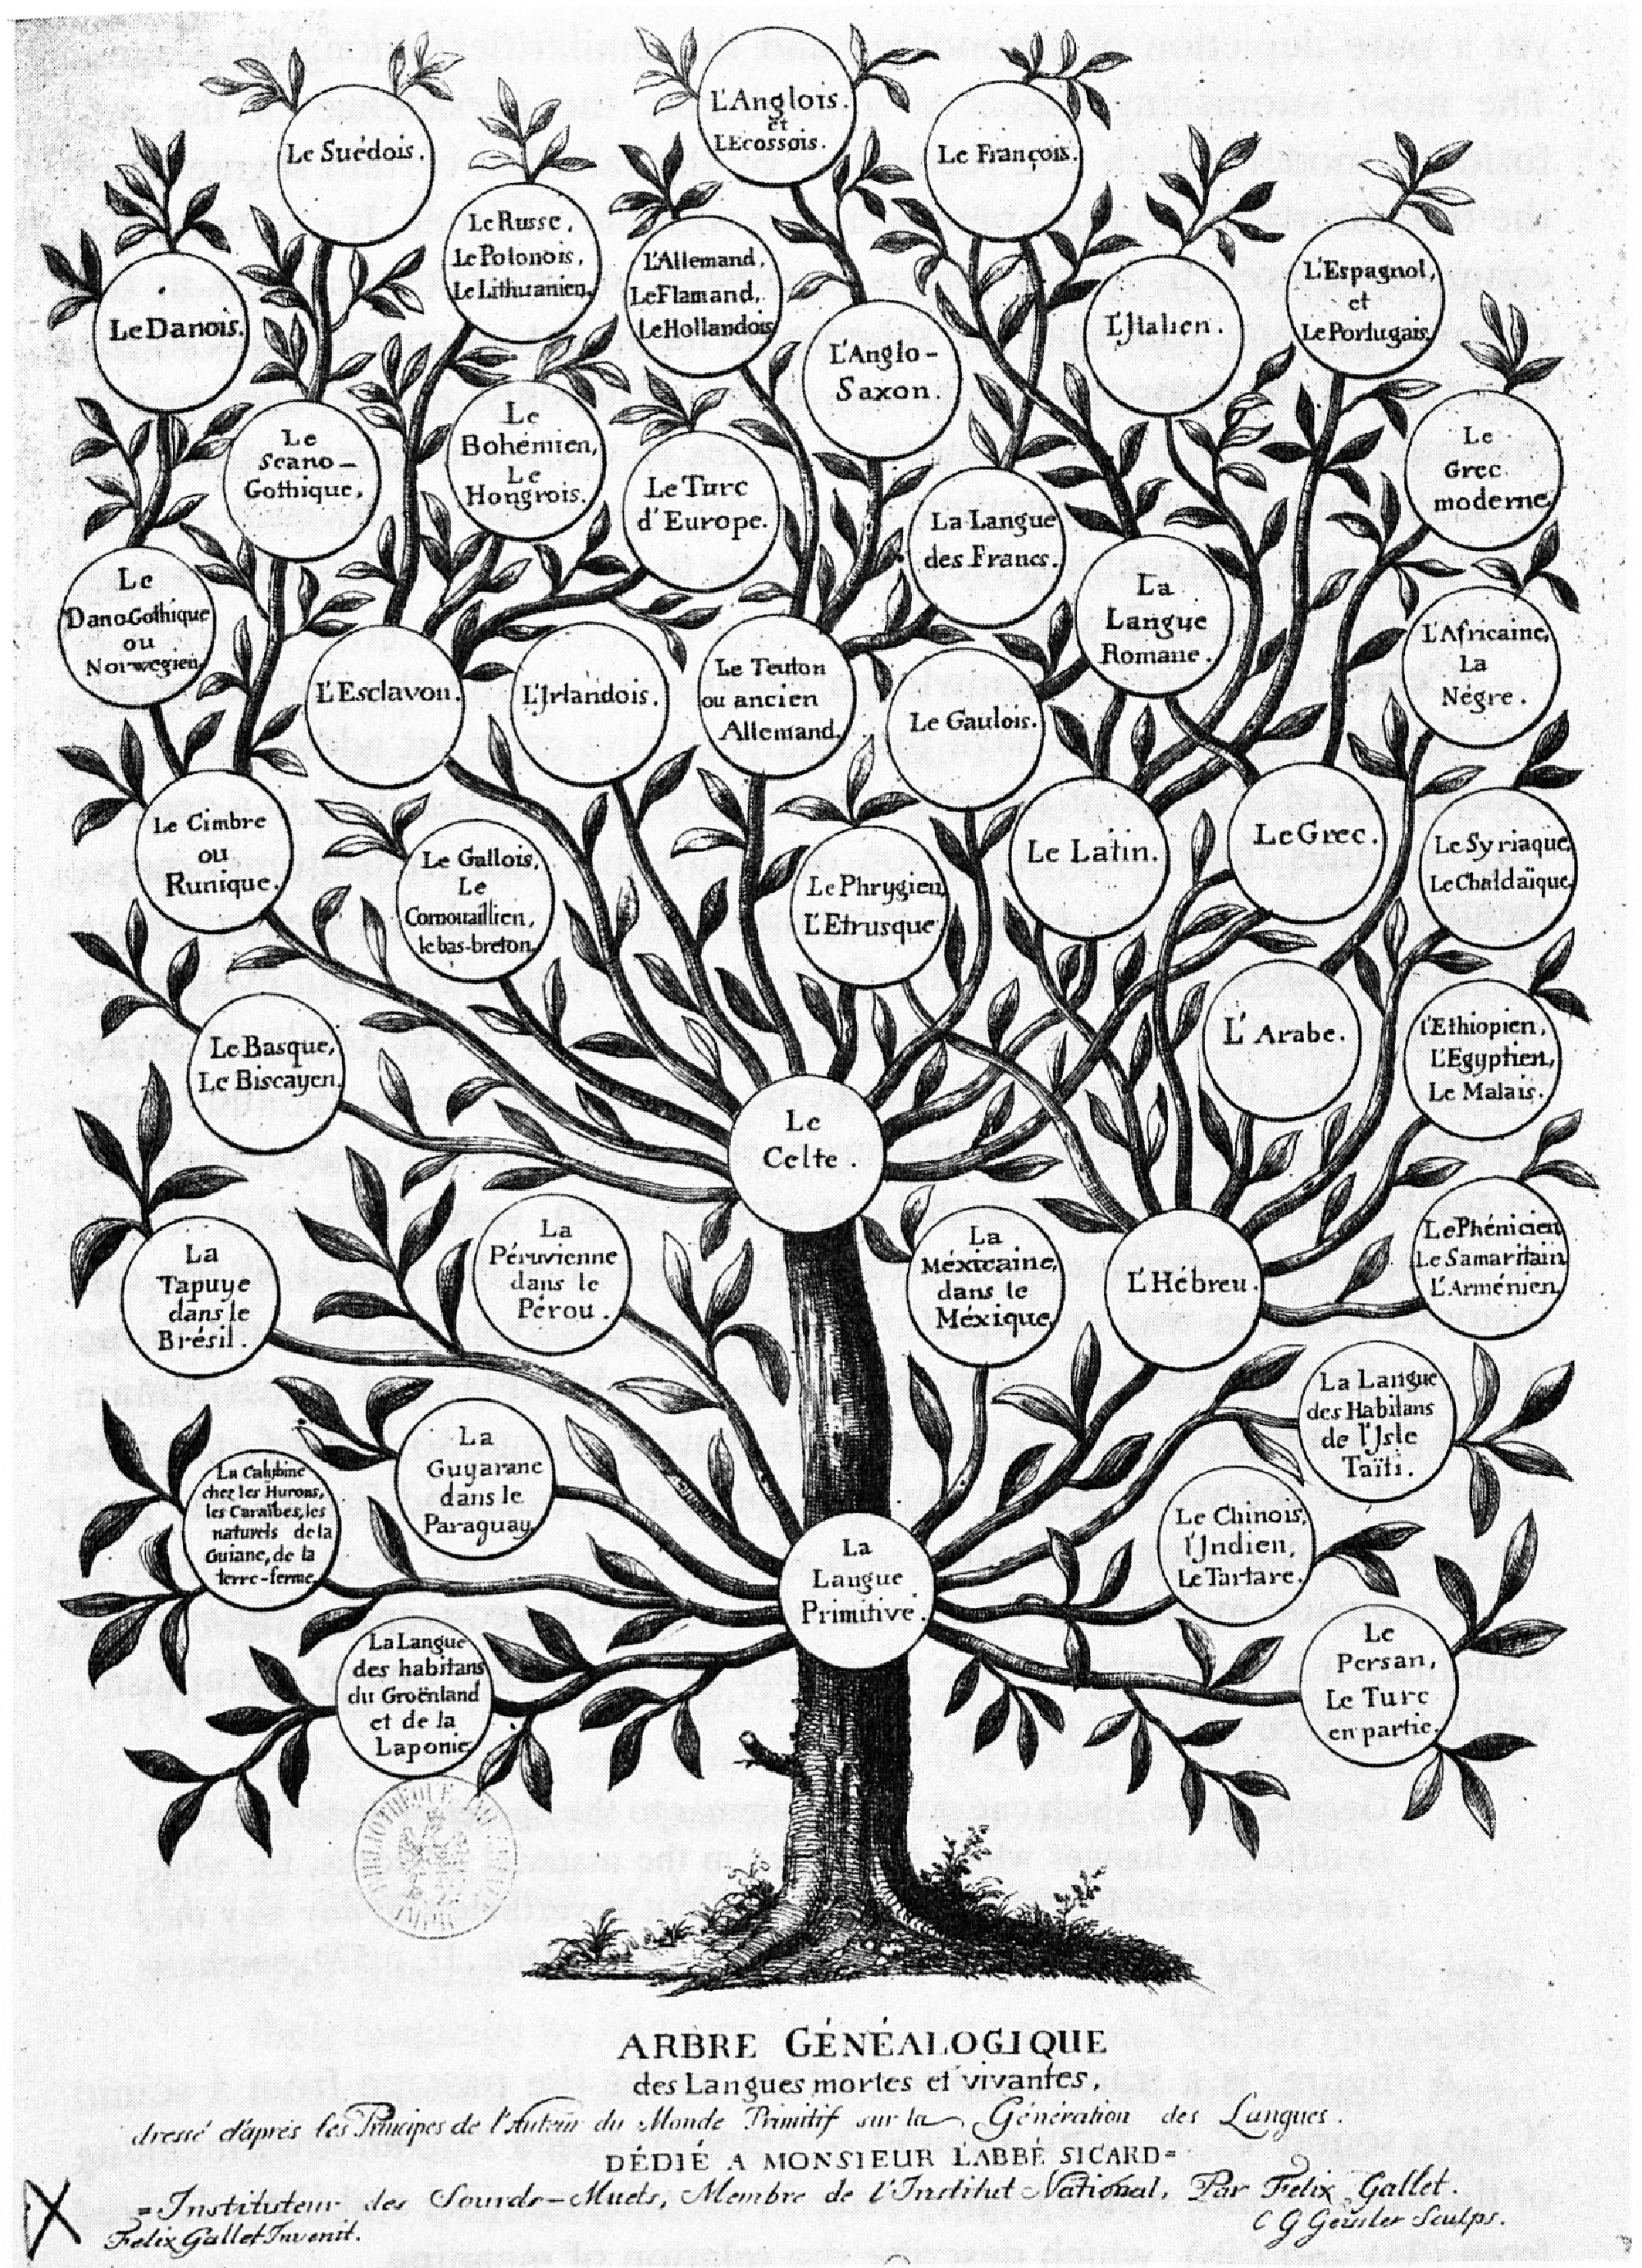
\includegraphics[width=0.5\textwidth]{img/arbre.jpg}
\includegraphics[width=0.5\textwidth]{img/schleicher.jpg}


\subsubsection{\texorpdfstring{{\ldots{} des
Seminarthemas}}{\ldots{} des Seminarthemas}}

\vspace{0.5cm}\par\noindent\textbf{Die Problematik des Sprachwandels}\vspace{0.5cm}

\includegraphics[width=0.5\textwidth]{img/hirt.jpg}
\includegraphics[width=0.5\textwidth]{img/bonfante.png}
\pagebreak


\vspace{0.5cm}\par\noindent\textbf{Die Wiederentdeckung der Bäume}\vspace{0.5cm}

\includegraphics[width=0.5\textwidth]{img/gray.jpg}
\includegraphics[width=0.5\textwidth]{img/ringe.png}

\includegraphics[width=\textwidth]{img/bridging-1.png}
\includegraphics[width=\textwidth]{img/bridging-2.png}

\includegraphics[width=\textwidth]{img/bridging-3.png}
\includegraphics[width=\textwidth]{img/bridging-4.png}
\pagebreak
\vspace{0.5cm}\par\noindent\textbf{Computergestützter Sprachvergleich}\vspace{0.5cm}

\includegraphics[width=\textwidth]{img/workflows.png}
\subsection{Allgemeines}

\subsubsection{\texorpdfstring{{\ldots{} zum
Programmieren}}{\ldots{} zum Programmieren}}

\vspace{0.5cm}\par\noindent\textbf{Warum ist es sinnvoll, programmieren zu können?}\vspace{0.5cm}

{Programmieren zu können ist immer dann sinnvoll, wenn man in seinem
Beruf oder den Studien, denen man nachgeht, häufig wiederholte,
redundante Operationen ausführen muss, die sich ebensogut automatisch
erledigen lassen würden.}



\vspace{0.5cm}\par\noindent\textbf{Warum ist es sinnvoll, programmieren zu können?}\vspace{0.5cm}

Wenn man zum Beispiel ein psycholinguistisches Experiment mit 200
Stimuli durchführen will, und wissen möchte, wie häufig die Wörter im
Durchschnitt vorkommen, dann kann man zur Webseite
\url{http://wortschatz.informatik.uni-leipzig.de/} gehen, wo die
Worthäufigkeit für eine Vielzahl von Wörtern verzeichnet ist, und jedes
der Wörter einzeln in das Suchfenster eingeben, um dessen Häufigkeit zu
ermitteln.



\vspace{0.5cm}\par\noindent\textbf{Warum ist es sinnvoll, programmieren zu können?}\vspace{0.5cm}

Dies wird dann mindestens zwei Stunden stumpfer Arbeit zur Folge haben,
während der man jedes einzelnen Wort kopiert, die Webseite auf- ruft,
die Häufigkeit kopiert und in eine Tabelle einträgt. Spätestens beim
dritten Experiment, das man durchführt, wird man diese Arbeit hassen und
sich Hiwis wünschen.



\vspace{0.5cm}\par\noindent\textbf{Daher ist es sinnvoll, programmieren zu können!}\vspace{0.5cm}

Alternativ kann man auch einfach programmieren: Die Leipziger
Wortschatzprojekt bietet eine Zusatzbibliothek für Python an
(\url{http://pypi.python.org/pypi/libleipzig}), mit deren Hilfe man ganz
schnell ein kleines Programm schreiben kann, das einem für eine
beliebige Liste von Wörtern in Sekundenschnelle alle Frequenzen (und
noch viel mehr Informationen, wenn man will) aus dem Internet
herunterlädt, und --- wenn man will, auch noch den Durchschnitt und die
Standardabweichung aller Frequenzen errechnet.



\vspace{0.5cm}\par\noindent\textbf{Daher ist es sinnvoll, programmieren zu können!}\vspace{0.5cm}

Die Eingabe ist dabei denkbar einfach. Um zum Beispiel die absolute
Frequenz des Wortes ``Python'' zu erhalten, muss man auf der
Kommandozeile einfach nur den folgenden Befehl eingeben:

\begin{verbatim}
>>> Frequencies("Python")

[(Anzahl: '129', Frequenzklasse: 17)]
\end{verbatim}


\subsubsection{\texorpdfstring{{\ldots{} zum Programmieren in der
Linguistik}}{\ldots{} zum Programmieren in der Linguistik}}

{ Die Linguistik, insbesondere die historische Linguistik, erlebt
derzeit einen Paradigmenwechsel. Während intuitives umfangreiches
Fachwissen, das Forscher sich über Jahre intensiven Studiums aneignen
mussten, bisher eine sehr große Rolle spielte, und formale Aspekte
lediglich als Gedankenspielereien präsentiert wurden, treten im Rahmen
der Big-Data-Bewegung nun mehr und mehr die empirischen Aspekte der
Disziplin in den Vordergrund. }



Die großen Datensammlungen und die leichte Zugänglichkeit von
Programmiertools machen es zusehends leichter, verschiedenste
Forschungsfragen empirisch zu untersuchen und zu überprüfen. Meiner
Meinung nach ist dies sehr wichtig, da die traditionelle Linguistik sich
viel zu wenig um die Empirie bemüht hat. Es ist jedoch wichtig, sich im
Klaren darüber zu sein, dass eine gute empirische Forschung
\vspace{0.5cm}\par\noindent\textbf{immer auf den Errungenschaften der traditionellen Linguistik\vspace{0.5cm}
aufbauen sollte}. Idealerweise praktizieren wir Linguistik als
{computergestützte Forschung}, das heißt, anstelle blind irgendwelchen
Algorithmen zu vertrauen, sollten wir Computermethoden entwickeln, die
helfen, traditionelle Ansätze zu modellieren und hochwertige Datensätze
für die empirische Forschung zu erstellen.

\subsection{Spezielles}

\subsubsection{\texorpdfstring{{\ldots{} zu Algorithmen, Skripten und
Programmen}}{\ldots{} zu Algorithmen, Skripten und Programmen}}

\vspace{0.5cm}\par\noindent\textbf{Was ist Programmieren?}\vspace{0.5cm}

\href{http://www.freenetpages.co.uk/hp/alan.gauld/german/tutwhat.htm}{Alan
Gauld} erklärt den Begriff Programmieren wie folgt:

\begin{quote}
Computer-Programmierung ist die Kunst, dass ein Computer das macht, was
du willst.
\end{quote}

{\href{http://de.wikipedia.org/wiki/Computerprogramm}{Wikipedia} ist ein
bisschen ausführlicher:}

\begin{quote}
Ein Computerprogramm oder kurz Programm ist eine Folge von den Regeln
der jeweiligen Programmiersprache genügenden Anweisungen, die auf einem
Computer ausgeführt werden können, um damit eine bestimmte
Funktionalität zur Verfügung zu stellen.
\end{quote}



\vspace{0.5cm}\par\noindent\textbf{Was ist Programmieren?}\vspace{0.5cm}

Etymologisch gesehen, bedeutet Programmieren so viel wie ``Vorschriften
erstellen'' und ist im Deutschen laut
\href{http://bibliography.lingpy.org?key=Kluge2002}{Kluge und Seebold
(2002)} zum ersten Mal seit dem 18. Jahrhunder bezeugt.

Entscheidend für das Programmieren, ist, was die Vorschriften betrifft,
dass diese ganz genau befolgt werden, denn so ergibt sich die
Möglichkeit, egal, ob das Programm nun von einem Menschen oder einem
Computer ausgeführt wird, dass das gewünschte Ergebnis immer erzielt
wird.



\vspace{0.5cm}\par\noindent\textbf{Was ist ein Algorithmus?}\vspace{0.5cm}

{Im \href{http://bibliography.lingpy.org?key=Kluge2002}{Kluge} finden
wir die Folgende Definition:}

\begin{quote}
\vspace{0.5cm}\par\noindent\textbf{Algorithmus.} Substantiv Maskulinum, ``Berechnungsverfahren'',\vspace{0.5cm}
peripherer Wortschatz, fachsprachlich (13. Jh., Form 16. Jh.), mhd.
algorismus. Onomastische Bildung. Entlehnt aus ml. algorismus, das das
Rechnen im dekadischen Zahlensystem und dann die Grund- rechenarten
bezeichnet. Das Wort geht zurück auf den Beinamen Al-Hwārizmī (''der
Chwa- resmier'', eine Herkunftsbezeichnung) eines arabischen
Mathematikers des 9. Jhs., durch dessen Lehrbuch die (indischen und
dann) arabischen Ziffern in Europa allgemein bekannt wurden. Das
Original des hier in Frage kommendes Buches ist verschollen, die ml.
Über- setzung ist Liber algorismi de practica arismetrice. Die
Schreibung mit

in Anlehnung an gr. arithmós ``Zahl''. {[}\ldots{}{]}
\end{quote}



\vspace{0.5cm}\par\noindent\textbf{Was ist ein Algorithmus?}\vspace{0.5cm}

{\href{http://bibliography.lingpy.org?key=Brassard1993}{Brassard und
Bratley (1993)} sind da weniger etymologisch:}

\begin{quote}
Das Concise Oxford Dictionary definiert einen Algorithmus als
``Verfahren oder Regeln für (speziell maschinelle) Berechnung''. Die
Ausführung eines Algorithmus darf weder sub- jektive Entscheidungen
beinhalten noch unsere Intuition und Kreativität fordern. Wenn wir über
Algorithmen sprechen, denken wir meistens an Computer.
Nichtsdestoweniger könn- ten andere systematische Methoden zur Lösung
von Aufgaben eingeschlossen werden. So sind zum Beispiel die Methoden
der Multiplikation und Division ganzer Zahlen, {[}\ldots{}{]} ebenfalls
Algorithmen. {[}\ldots{}{]} Es ist sogar möglich, bestimmte Kochrezepte
als Algorithmen aufzufassen, vorausgesetzt, sie enthalten keine
Anweisungen wie ``nach Geschmack salzen''.
\end{quote}



\begin{itemize}
\itemsep1pt\parskip0pt\parsep0pt
\item
  Ein Algorithmus ist eine geordnete Sammlung von Verfahren, mit deren
  Hilfe eine Aufgabe (ein Problem) eindeutig gelöst werden kann.
\item
  Ein Programm ist eine \emph{Implementierung} von Algorithmen mit Hilfe
  einer speziellen Programmiersprache.
\item
  Ein Skript ist ein Programm, das in einer interpretierten
  Programmiersprache (einer Skriptsprache) geschrieben wurde. Alle
  Programme, die mit Python oder JavaScript erstellt werden, sind
  demnach Skripte.
\end{itemize}


\subsubsection{\texorpdfstring{{\ldots{} zur Grundausstattung fürs
Programmieren}}{\ldots{} zur Grundausstattung fürs Programmieren}}

\vspace{0.5cm}\par\noindent\textbf{Texteditoren}\vspace{0.5cm}

Um Skripte zu schreiben, benötigen wir einen guten
\href{http://de.wikipedia.org/wiki/Texteditor}{Texteditor}. Das ist
nicht das gleiche wie Word oder LibreOffice, sondern ein Editor, der
reinen Text schreibt. Aus Zeitgründen erwarte ich von allen Teilnehmern
des Seminars, dass sie sich eigenständig einen guten Texteditor zulegen,
um Skripte zu schreiben. Ferner ist zu beachten, dass alle Dateien in
\href{https://de.wikipedia.org/wiki/UTF-8}{UTF-8} abgespeichert werden
solltet.

Ich selbst schreibe meine Skripte alle mit \href{http://vim.org}{VIM}.
Weitere populäre Texteditoren sind:

\begin{itemize}
\itemsep1pt\parskip0pt\parsep0pt
\item
  \href{https://www.gnu.org/software/emacs/}{GNU Emacs}: der natürliche
  Feind von allen, die gerne VIM benutzen
\item
  \href{http://de.wikipedia.org/wiki/Notepad++}{Notepad++}: ein relativ
  ordentlicher Texteditor für Windows-Benutzer
\end{itemize}



\vspace{0.5cm}\par\noindent\textbf{Versionsverwaltungssoftware}\vspace{0.5cm}

Wer größere Projekte schreibt, kommt ohne sie nicht aus: die Software
zur Versionsverwaltung. Ich selbst verwende
\href{http://de.wikipedia.org/wiki/Git}{Git} für meine Arbeit, da es
sich wunderbar mit \href{http://github.org}{GitHub} integrieren lässt,
und Daten dadurch auch anderen Nutzern zur Verfügung gestellt werden
können. Für das Seminar setze ich voraus, dass jeder Teilnehmer sich
grundlegend mit den Ideen hinter Git auseinandersetzt. Um an bestimmte
Resourcen zu gelangen, die ich anbiete, wird ferner ein GitHub Account
benötigt werden. Ich empfehle ohnehin allen Programmierinteressierten,
sich einen GitHub Account anzulegen, da sich GitHub mehr und mehr zum
Standard für kollaboratives Arbeiten entwickelt (was nicht heißt, dass
ich es gut finde, dass dahinter ein Konzern steckt!).



\vspace{0.5cm}\par\noindent\textbf{Möglichkeiten zum Datenhosting}\vspace{0.5cm}

Wer als Linguist programmiert möchte irgendwann auch seinen Sourcecode
anderen Nutzern zur Verfügung stellen. Das ist sehr leicht möglich mit
Hilfe neuer gemeinnütziger Anbieter. Ich empfehle in diesem Zusammenhang
\href{http://zenodo.org}{Zenodo}. Man kann sich mit seinem GitHub
Account anmelden, und seinen Code entweder automatisch von Zenodo hosten
lassen, oder ihn direkt manuell hochladen. Zenodo garantiert
Langzeitarchivierung, ist kostenlos (weil gemeinnützig), und erlaubt bis
zu zwei Gigabyte an Daten pro Projekt. Außerdem bekommt man von Zenodo
immer automatisch einen
\href{http://de.wikipedia.org/wiki/Digital_Object_Identifier}{Digital
Object Identifier}, was gewährleistet, dass die Daten im Netz auffindbar
und unmissverständlich referenzierbar sind.


\subsubsection{\texorpdfstring{{\ldots{} zu Python und
JavaScript}}{\ldots{} zu Python und JavaScript}}

\vspace{0.5cm}\par\noindent\textbf{Vorzüge von Python (frei nach\vspace{0.5cm}
\href{http://bibliography.lingpy.org?key=Bassi2010}{Bassi (2010:10)})}

\begin{itemize}
\itemsep1pt\parskip0pt\parsep0pt
\item
  \textbf{Readability}: Python is a ``human-readable language''
\item
  \textbf{Built-in features}: Python comes with ``batteries included''
\item
  \textbf{Availability of third-party modules}: plotting, game
  development, databases, etc. to model real-world data
\item
  \textbf{multi-paradigm}: can be used as a procedural and
  object-oriented programming language
\item
  \textbf{extensibility}: Python can be connected to many other
  languages
\item
  \textbf{open source}: liberal open source license, also for commercial
  use
\item
  \textbf{cross-platform}: works on any computer (even Windows)
\item
  \textbf{thriving community}: ask whatever question on
  \href{http://stackoverflow.com}{stackoverflow}, you'll get an answer
  in most of the cases
\end{itemize}



\vspace{0.5cm}\par\noindent\textbf{Vorzüge von JavaScript (frei nach Meinung von mir)}\vspace{0.5cm}

\begin{itemize}
\itemsep1pt\parskip0pt\parsep0pt
\item
  \textbf{cross-platform}: JavaScript ist die einzig wirkliche
  Cross-Platformsprache, weil jeder, der einen Webbrowser hat, sie auch
  hat
\item
  \textbf{schön anzusehen}: JavaScript ist sehr hilfreich, wenn man
  Programme schreiben will, die optisch ansprechend sind
\item
  \textbf{leicht zu verwenden (für den Anwender)}: JavaScript macht es
  dem Anwender leicht (dem Programmierer aber leider eher schwer)
\item
  \textbf{Schönheit ist nicht alles}: JavaScript ist eine durchweg
  hässliche Sprache. Dennoch kann man sich mit ihr ganz ordentlich
  arrangieren.
\item
  \textbf{große Unterstützergemeinschaft}: wahrscheinlich sogar größer
  als die von Python: man findet sehr schnell antworten zu Fragen im Web
\item
  \textbf{viele Third-Party-Modules}: es gibt eine Unmenge von Modulen,
  auf die man zurückgreifen kann, und noch viel mehr kurze Beispiele
\end{itemize}



Mit Python und JavaScript hat man zwei unheimlich Mächtige Tools zur
Hand, die es einem erlauben, Daten nicht nur auf hochwertige Weise zu
analysieren, sondern die Ergebnisse auch noch interaktiv zu
präsentieren. Für die moderne, computergestützte Wissenschaft, ist es
ein großer Vorteil, über Grundwissen in beiden Sprachen zu verfügen.



\section{Erste Schritte in Python}
\hyperdef{}{tilda}{}

\subsection{\texorpdfstring{{Allgemeines zu
Python}}{Allgemeines zu Python}}

\subsubsection{\texorpdfstring{{Herkunft}}{Herkunft}}

\href{http://python.org}{Python}

\begin{itemize}
\itemsep1pt\parskip0pt\parsep0pt
\item
  {wurde Anfang der 1990er Jahre von Guido van Rossum entwickelt}
\item
  {erhielt seinen Namen in Anspielung auf die Monty Pythons}
\item
  {erschien 1994 in der ersten Version 1.0}
\item
  {erschien 2000 in der Version 2.0, die viele Neuerungen enthielt}
\item
  {erschien 2008 in der Version 3.0, die nicht mehr kompatibel mit 2.0
  ist, eine Vielzahl von Verbesserungen aufweist und von uns verwendet
  wird}
\end{itemize}


\subsubsection{\texorpdfstring{{Charakteristik}}{Charakteristik}}

\href{http://python.org}{Python}

\begin{itemize}
\itemsep1pt\parskip0pt\parsep0pt
\item
  {ist eine universelle, interpretierte höhere Programmiersprache}
\item
  {ist sehr stark auf gute Lesbarkeit ausgerichtet}
\item
  {relativ einfach zu erlernen}
\item
  {sehr flexibel (unterstützt objektorientierte und funktionale
  Programmierung)}
\item
  {bietet in der Version 3 endlich eine volle Unicode-Unterstützung}
\item
  {besticht durch einfache Syntax und relativ wenige Schlüsselwörter}
\item
  {ist eine wunderschöne Sprache}
\end{itemize}


\subsubsection{\texorpdfstring{{Installation}}{Installation}}

\begin{itemize}
\itemsep1pt\parskip0pt\parsep0pt
\item
  {Download unter \url{http://python.org} (wir verwenden ausschließlich
  Python 3 im Rahmen des Seminars!)}
\item
  {Installationsanleitung unter
  \url{https://www.python.org/about/gettingstarted/}}
\item
  {die Installation sollte generell problemlos auf fast allen
  Plattformen verlaufen}
\end{itemize}

\subsection{\texorpdfstring{{Bibliotheken und
Entwicklertools}}{Bibliotheken und Entwicklertools}}

\subsubsection{\texorpdfstring{{Allgemeines}}{Allgemeines}}

\href{http://de.wikipedia.org/wiki/Programmbibliothek}{Wikipedia} zur
``Programmbibliothek'':

\begin{quote}
Eine Programmbibliothek bezeichnet in der Programmierung eine Sammlung
von Programmfunktionen für zusammengehörende Aufgaben. Bibliotheken sind
im Unterschied zu Programmen keine eigenständig lauffähigen Einheiten,
sondern Hilfsmodule, die Programmen zur Verfügung gestellt werden.
\end{quote}

\vspace{0.5cm}\par\noindent\textbf{Installation von Python-Bibliotheken mit\vspace{0.5cm}
\href{http://pypa.io}{pip}}

Die Installation von Python-Bibliotheken ist relativ einfach, wenn man
auf das Installationstool \emph{pip} (``pip installs packages'')
zurückgreift. Dieses ist bei den neuesten Pythonversionen (3.4) bereits
vorinstalliert, und kann daher direkt verwendet werden. Die verwendung
ist denkbar einfach. In der Kommandozeile (``cmd'' in der Suchleiste bei
Windows eingeben) gibt man einfach Folgendes ein:

\begin{verbatim}
$ pip install packagename
\end{verbatim}

Daraufhin wird die Bibliothek dann installiert.

\subsubsection{Empfohlene Python-Bibliotheken}
\begin{itemize}
\itemsep1pt\parskip0pt\parsep0pt
\item
  {\href{http://numpy.org}{NumPy}, ``Numeric Python'',
  \url{http://numpy.org}: Sehr gute Bibliothek, die eine Vielzahl
  effizienter numerischer Berechnungen erlaubt und häufig als Grundlage
  für weitere Bibliotheken gefordert wird. }
\item
  {\href{http://scipy.org}{SciPy}, ``Scientific Python'',
  \href{http://scipy.org}{http:/scipy.org}: Sehr wichtige (leider etwas
  langsame) Bibliothek für wissenschaftliche Programmierung. }
\item
  {\href{http://matplotlib.org}{Matplotlib},
  \url{http://matplotlib.org}: Exzellente Bibliothek für das Erstellen
  hochwertiger Plots von Daten.}
\item
  {\href{http://networkx.org}{Networkx}, \url{http://networkx.org}: Sehr
  gute Bibliothek für Netzwerkkalkulationen.}
\item
  {\href{http://lingpy.org}{LingPy}, ``Linguistic Python'',
  \url{http://lingpy.org}: Bibliothek zur Durchführung von quantitativen
  Analysen in der historischen Linguistik (Download unter:
  \url{https://github.com/lingpy/lingpy/releases/tag/v2.4.1-alpha}).}
\end{itemize}


\subsubsection{\texorpdfstring{{Empfohlene
Entwicklertools}}{Empfohlene Entwicklertools}}

\begin{itemize}
\item
  {\href{http://ipython.org}{IPython}, \url{http://ipython.org}: Sehr
  gutes Kommandozeileninterpreter für Python, der vor allem auch das
  Testen von Code ungemein erleichtert. }
\item
  {Installation unter Windows (kann etwas kompliziert werden, aber Sie
  sollten das schon schaffen!):
  \url{http://ipython.org/ipython-doc/2/install/install.html\#windows}}
\item
  {Installation unter Linux/Ubuntu: }

\begin{verbatim}
$ sudo apt-get install ipython3
\end{verbatim}
\item
  {Installation unter Archlinux: }

\begin{verbatim}
$ sudo pacman -S ipython
\end{verbatim}
\end{itemize}

\subsection{\texorpdfstring{{Ein erstes
Programmierbeispiel}}{Ein erstes Programmierbeispiel}}

\subsubsection{\texorpdfstring{{Das Problem}}{Das Problem}}

\begin{quote}
Karlheinz, ein Düsseldorfer Student der Lingustik im 20. Semester, hat
auf einer Mediziner-Party in Köln eine Medizinstudentin kennengelernt,
die ihr Physikum bereits abgeschlossen hat, und möchte sie gerne
wiedersehen. Dummerweise kann er sich jedoch nicht mehr genau daran
erinnern wie sie heißt. Ihr Nachname klang irgendwie nach {{[}maiɐ{]}},
und ihr Vorname war irgendwas in Richtung {{[}krɪstiːnə{]}}, jedoch weiß
er nicht, welche Schreibung er zugrunde legen soll.
\end{quote}



\begin{quote}
Zufällig hat er eine Liste mit den wirklichen Namen und den
dazugehörigen Facebook-Namen von allen Bürgern aus Köln und Umgebung als
Excel-Tabelle auf seinem Computer zu Hause. Wenn er jetzt noch ein
Verfahren finden könnte, das ihm alle Namen anzeigt, die wie
{{[}krɪstiːnə maiɐ{]}} klingen, dann wäre es sicherlich ein Leichtes,
herauszufinden, wo die unbekannte Studentin ihre Tierversuche
veranstaltet, und sie mit einem Pausenkaffee von . Starbucks zwischen
Frosch und Kaninchen zu überraschen\ldots{}
\end{quote}


\subsubsection{\texorpdfstring{{Der Algorithmus}}{Der Algorithmus}}

{ Die Lösung besteht darin, alle Namen, die auf der Liste auftauchen, in
ein anderes Format umzuwandeln, welches den Sprachklang der Wörter
wiedergibt und nicht ihre Schreibung. Ein Algorithmus, der für diesen
Zweck geschaffen wurde, ist die sogenannte ``Kölner Phonetik'' (vgl.
\href{http://bibliography.lingpy.org?key=Postel1969}{Postel 1969}). Die
Kölner Phonetik wandelt Wörter der deutschen Sprache in einen
phonetischen Kode um, mit dessen Hilfe auch Wörter, die unterschiedlich
geschrieben werden, aber gleich klingen, verglichen werden können. So
werden die beiden Namen \emph{Christina Maier} und \emph{Kirsten Mayr}
durch den Algorithmus jeweils in die gleiche Zahlenfolge ``47826-67''
umgewandelt.}



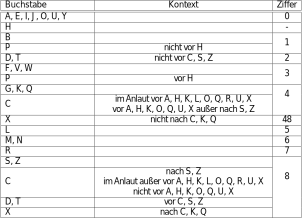
\includegraphics[width=\textwidth]{img/kphon.pdf}


\vspace{0.5cm}\par\noindent\textbf{Das Verfahren}\vspace{0.5cm}

\begin{enumerate}
\itemsep1pt\parskip0pt\parsep0pt
\item
  Wandle jeden Buchstaben schrittweise um und beachte die Kontextregeln.
\item
  Reduziere alle mehrfach hintereinander auftauchenden Ziffern auf eine.
\item
  Entfernen die Ziffer ``0'' an allen Stellen des Wortes, außer am
  Anfang.
\end{enumerate}


\vspace{0.5cm}\par\noindent\textbf{Aufgabe an alle Seminarteilnehmer}\vspace{0.5cm}

Wenden Sie die Kölner Phonetik auf Ihren Vor- und Nachnamen an und
dokumentieren Sie dabei explizit, welche Schritte Sie dabei durchführen.
Warum ist das Verfahren komplizierter, als man am Anfang vermuten
könnte?


\subsubsection{\texorpdfstring{{Die
Python-Implementierung}}{Die Python-Implementierung}}

Die Kölner Phonetik ist in Python von Robert Schindler implementiert
worden und unter der URL (http://pypi.python.org/pypi/kph/0.3)
erhältlich. Wir ignorieren vorerst die Details der Umsetzung und
konzentrieren uns auf die Anwendung. Die Installation ist dank ``pip''
denkbar einfach:

\begin{verbatim}
$ pip install kph
\end{verbatim}

{Die Verwendung auch:}

\begin{verbatim}
>>> import kph
>>> kph.encode("Mattis List")
'628582'
\end{verbatim}

{Aber wie können wir eine lange Liste von Namen abfragen, ohne jeden
Namen einzeln in der Konsole eingeben zu müssen?}

{Richtig, wir brauchen ein Skript!}


\vspace{0.5cm}\par\noindent\textbf{Aufbau von Python-Skripten: Shebang und Kodierung}\vspace{0.5cm}

Die erste Zeile von Python-Skripten sieht oft wie folgt aus:

\begin{verbatim}
#! /usr/bin/env python
# *-* coding:utf-8 *-*

YOUR CODE HERE
\end{verbatim}

Die erste Zeile, die sogenannte
\href{http://de.wikipedia.org/wiki/Shebang}{Shebang line}, erlaubt es,
das Programm durch Doppelklick in Linux- und Mac-Systemen (``unixoide
Systeme'') auszuführen. Die zweite Zeile legt die Kodierung fest und
erlaubt es, bei der Verwendung von Python-2 Programmen, alle Arten von
nicht-ASCII Zeichen zu verwenden. Streng genommen brauchen wir aber
keine der Funktionen, da wir Programme auf Unix-Computern auch leicht
über die Konsole ausführen können, und Python3 UTF-8 voll unterstützt.



\vspace{0.5cm}\par\noindent\textbf{Aufbau von Python-Skripten: Kommentare}\vspace{0.5cm}

\begin{verbatim}
# Dies ist eine Kommentarzeile,
# durch welche es möglich ist, Dinge in das
# Programm zu schreiben, die nachher
# nicht ausgeführt werden.

# Man kann Kommentare Überall einsetzen, man 
# muss aber beachten, dass, wenn man
# sie einsetzt, alles was hinter dem Kommentar-Zeichen folgt, nicht mehr
# interpretiert wird.

1 + 1 # wird hier interpretiert
# 1 + 1 wird nicht interpriert
1 + # ruft einen Fehler hervor, weil das "+" ohne Gegenstück ist
\end{verbatim}

\begin{verbatim}
"Alternativ kann man Dinge auch in Anführungsstriche setzen."

"""
Sicherer ist es allerdings, drei Anführungsstriche auf
einmal zu verwenden, weil man dann auch Anführungsstriche
inerhalb des Kommentars benutzen kann, bzw. auch über
mehrere Zeilen hinweg schreiben kann.
"""
\end{verbatim}



\vspace{0.5cm}\par\noindent\textbf{\href{code/hallo_welt.py}{Die Print-Funktion}}\vspace{0.5cm}

\begin{verbatim}
# file: hallo_welt.py
print("Hallo Welt!")
\end{verbatim}

\begin{verbatim}
$ python3 hallo_welt.py
Hallo Welt!
\end{verbatim}

\vspace{0.5cm}\par\noindent\textbf{\href{code/test_kph.py}{Einbinden von Modulen (Bibliotheken)}}\vspace{0.5cm}

\begin{verbatim}
# file: test_kph.py

import kph 
# importiert die Kölner Phonetik, vorher kann man
# die Bibliothek nicht verwenden

print(kph.encode('Monty Python'))
\end{verbatim}

\begin{verbatim}
$ python3 test_kph.py
662126
\end{verbatim}



\vspace{0.5cm}\par\noindent\textbf{Einige kurze Ideen zum Experimentieren und Nachdenken}\vspace{0.5cm}

\begin{enumerate}
\itemsep1pt\parskip0pt\parsep0pt
\item
  {Experimentieren Sie mit der Kölner Phonetik. Welche Ausgaben erhalten
  Sie, wenn Sie}

  \begin{itemize}
  \itemsep1pt\parskip0pt\parsep0pt
  \item
    {eine Zahl in Anführungsstrichen,}
  \item
    {eine Zahl ohne Anführungsstriche, oder}
  \item
    {Buchstaben mit diakritischen Zeichen (``áłň'') eingeben?}
  \end{itemize}
\item
  {Gibt man statt
  \verb|"Kirsten"|,\verb|"Maier"|
  die Zeile \texttt{encode("Kirsten\ Maier")} ein, verändert sich die
  Ausgabe. Woran liegt das?}
\item
  {Was brauchen wir (welche Routinen, Verfahren), um alle Daten aus der
  Excel-Tabelle von Karlheinz einlesen und in ihre Werte entsprechend
  der Kölner Phonetik umwandeln zu können?}
\end{enumerate}



\section{Erste Schritte in JavaScript}
\hyperdef{}{tilda}{}

\subsection{\texorpdfstring{{Allgemeines zu
JavaScript}}{Allgemeines zu JavaScript}}

\subsubsection{\texorpdfstring{{Herkunft}}{Herkunft}}

\href{http://de.wikipedia.org/wiki/JavaScript}{JavaScript}

\begin{itemize}
\itemsep1pt\parskip0pt\parsep0pt
\item
  {ist eine Skriptsprache, die speziell für dynamisches HTML in
  Webbrowsern entwickelt wurde}
\item
  {verändert Inhalte von Webseiten, reagiert auf Benutzereingaben, und
  erweitert die Möglichkeiten von HTML und CSS}
\item
  {ist ein abtrünniges Kind von C, was die hässliche Syntax angeht und
  hat mit Java selbst sehr wenig zu tun (obwohl die Syntax von Java auch
  sehr hässlich ist)}
\item
  {wurde ursprünglich von Netscape entwickelt und im Jahre 1996 in der
  Version 1.1 veröffentlicht}
\end{itemize}


\subsubsection{\texorpdfstring{{Charakteristik}}{Charakteristik}}

\href{http://de.wikipedia.org/wiki/JavaScript}{JavaScript}

\begin{itemize}
\itemsep1pt\parskip0pt\parsep0pt
\item
  {hat eine sehr hässliche Syntax}
\item
  {ist prinzipiell nicht sehr schwer zu erlernen, sieht aber hässlich
  aus}
\item
  {erlaubt es den Benutzern, sehr, sehr hässlichen Kode zu schreibne}
\item
  {ist am Anfang sehr gewöhungsbedürftig, bis man begriffen hat, wie die
  Interaktion zwischen HTML, CSS, und JavaScript abläuft}
\item
  {ist generell ``innen pfui, außen hui''}
\item
  {macht des dem Benutzer sehr schwer, modularen Kode zu schreiben}
\end{itemize}


\subsubsection{\texorpdfstring{{Installation}}{Installation}}

{ JavaScript ist fester Bestandteil gängiger Webbrowser, wie
\href{http://de.wikipedia.org/wiki/Mozilla_Firefox}{Firefox},
\href{http://de.wikipedia.org/wiki/Google_Chrome}{Chrome}, oder
\href{http://de.wikipedia.org/wiki/Apple_Safari}{Safari}. Im
\href{http://de.wikipedia.org/wiki/Internet_Explorer}{Internet-Explorer}
ist JavaScript angeblich auch vorinstalliert, jedoch laufe viele Apps
sehr viel schlechter als gewünscht, weil Microsoft sich mal wieder
qualitativ von den anderen Anbietern abgrenzen muss. }

\subsection{\texorpdfstring{{Bibliotheken und
Entwicklertools}}{Bibliotheken und Entwicklertools}}

\subsubsection{\texorpdfstring{{Webbrowser}}{Webbrowser}}

{ Ich empfehle, beim Entwickeln von JavaScript-Applikationen
grundsätzlich auf einen der gängigen Unix-Browser
(\href{http://de.wikipedia.org/wiki/Mozilla_Firefox}{Firefox},
\href{http://de.wikipedia.org/wiki/Google_Chrome}{Chrome}, oder
\href{http://de.wikipedia.org/wiki/Apple_Safari}{Safari})
zurückzugreifen. Firefox und Chrome, welche ich beide regelmäßig
verwende, unterscheiden sich in den Funktionen, die sie bieten. Firefox
erlaubt bestimmte Dateizugriffe, ohne die Applikation über einen Server
laufen zu lassen, was die Entwicklung von Applikationen erleichtert.
Chrome hat Vorteile im Layout und im Debugging. Grundsätzlich sollten
alle Applikationen mindestens auf Firefox und Chrome getestet werden, da
es hier mitunter zu bestimmten Unterschieden kommen kann. Auch
unerwartete Fehler können in einem Webbrowser auftauchen, im anderen
aber nicht. }


\subsubsection{\texorpdfstring{{Bibliotheken}}{Bibliotheken}}

\par\noindent\textbf{Empfohlene Frameworks:}

\begin{itemize}
\itemsep1pt\parskip0pt\parsep0pt
\item
  {\href{http://jquery.com}{jQuery}: eine der am weitesten verbreiteten
  JavaScript-Bibliotheken, die viele Erweiterungen und Erleichterungen
  bietet und als Grundlage zahlreicher Plugins dient. Aufgrund der Größe
  von jQuery sollte man sich jedoch für jedes Projekt überlegen, ob man
  die Bibliothek auch wirklich braucht, denn auch JavaScript allein
  bietet viele Möglichkeiten, kurzen und knackigen Kode zu schreiben.}
\item
  {\href{http://d3js.org}{d3}: Eine wunderbare Bibliothek zur
  Datenvisualisierung, ein bisschen gewöhnungsbedürftig in der
  Anwendung, aber unheimlich schön in den Ergebnissen. Entwickelt wurde
  die Bibliothek vorrangig von Mike Bostock, der für die New York Times
  arbeitet, die seine Pionierarbeit der interaktiven Visualisierung
  sponsort.}
\end{itemize}


\subsubsection{\texorpdfstring{{Entwicklertools}}{Entwicklertools}}

Man kann JavaScript auch in der Konsole ausführen (die selbst in
JavaScript geschrieben wurde):

{ Zum Testen bietet sich \href{http://nodejs.org}{node.js} an: Dieses
Paket erlaubt es, JavaScript Kode in Skripten auszuführen und bietet
auch eine interaktive Konsole. Der Vorteil von node.js ist, dass man
Skripte testen kann, ohne den ansonsten erforderlichen HTML/CSS-Überbau
zugrunde legen zu müssen. }

\subsection{\texorpdfstring{{Ein erstes
Programmierbeispiel}}{Ein erstes Programmierbeispiel}}

\subsubsection{\texorpdfstring{{Die Kölner Phonetik in
JavaScript}}{Die Kölner Phonetik in JavaScript}}

{ Es existiert natürlich bereits eine Implementierung der Kölner
Phonetik für JavaScript, implementiert von J. Tillmann:
\url{https://github.com/jtillmann/colophoneticjs}. Diese Version wurde
für die Zwecke unseres Seminars leicht umgeschrieben, so dass wir sie in
ähnlicher Weise, wie die Python-Version der Kölner Phonetik verwenden
können. Der resultierende Source Code, ein Skript mit Namen
\href{https://github.com/LinguList/pyjs-seminar/blob/master/website/code/kph.js}{kph.js}
befindet sich auf der Projektwebseite und kann dort heruntergeladen
werden. Er wurde ebenfalls bereits in die Terminal-Applikation
integriert. }



\par\noindent\textbf{Kölner Phonetik mit Hilfe des
\href{../demos/console.html}{Web-Terminals}:}

\begin{verbatim}
js> kph.encode('Mayer');
67
\end{verbatim}

{ }



\par\noindent\textbf{Kölner Phonetik mit node.js:}

{Einbinden von kph.js:}

\begin{verbatim}
> kph = require('./js/kph.js') /* Im Order demos/ */
{ encode: [Function] }
\end{verbatim}

{Anwenden:}

\begin{verbatim}
> kph.encode('Müller-Lüdenscheidt');
'65752682'
> kph.encode('Muller-Ludenscheidt Sebastian Bach')
65752682 81826 14
\end{verbatim}



Die Verwendung in der Konsole ist aber noch nicht alles! Viel
interessanter wird es ja, wenn man den Kode gleich auf einer Webseite
einsetzen kann, zum Beispiel als interaktive Applikation.

Dafür brauchen wir zunächst eine HTML-Eingabe und Ausgabe, die wir in
einer HTML-Seite (mit Standard-Head-Body Struktur) wie folgt
unterbringen können:

\begin{verbatim}

OK</>
\end{verbatim}

{Die Ausgabe sieht dann auf der Webseite wie folgt aus:}

OK

\hyperdef{}{opt}{}



Um eine bestimmte JavaScript-Bibliothek ausführen zu können, müssen wir
sie im Header der HTML-Datei (oder an einer beliebigen anderen Stelle)
einbinden, was wie folgt aussieht:

\begin{verbatim}
<html>
  <head>
    
    
  </head>
  <body>
    
    GIB MIR DIE KPH!
    
  </body>
</html>
\end{verbatim}



Dann brauchen wir noch eine JavaScript Funktion, die mit HTML
kommuniziert:

\begin{verbatim}
// Funktion greift auf die HTML-Datei zu und Berechnet
// die Werte für die Kölner Phonetik
function showKPH() {
  /* get the input button element */
  var ipt = document.getElementById('ipt');
  /* get the input value */
  var ipt_val = ipt.value;
  /* convert to Kölner Phonetik */
  var converted_values = kph.encode(ipt_val);
  /* write to html page */
  var opt = document.getElementById('opt');
  opt.innerHTML = converted_values;
}
\end{verbatim}

{Beachten Sie, dass es zwei Arten in JS gibt, um Kommentare einzufügen,
den Doppelslash (//), der den Rest einer Zeile auskommentiert, und die
Kombination von Slash mit Asterisk (/* und */), mit denen man auch über
Zeilen hinaus auskommentieren kann. }



Diese Datei können wir entweder als separates Skript abspeichern und in
HTML einbinden,

\begin{verbatim}
<html>
  ...
    
    
  </body>
\end{verbatim}

oder wir können sie direkt zwischen die Skript-Tags schreiben

\begin{verbatim}
<html>
  ...
    
    
function showKPH() {
  var ipt = document.getElementById('ipt');
  var ipt_val = ipt.value;
  var converted_values = kph.encode(ipt_val);
  var opt = document.getElementById('opt');
  opt.innerHTML = converted_values;
}
    
  </body>
\end{verbatim}



Und so sieht das Ganze dann in Aktion aus:


\section{Datentypen und Variablen}
\hyperdef{}{tilda}{}

\subsection{\texorpdfstring{{Variablen}}{Variablen}}

\subsubsection{\texorpdfstring{{\ldots{} im
Allgemeinen}}{\ldots{} im Allgemeinen}}

\par\noindent\textbf{Was ist eine Variable?}

\begin{itemize}
\itemsep1pt\parskip0pt\parsep0pt
\item
  {\emph{Variable} ist das Substantiv zu \emph{variabel}, welches auf
  Latein \emph{variabilis} ``veränderbar'' zurückgeht.}
\item
  {Eine Variable ist also etwas, das änderbar ist.}
\item
  {Johnny Depp ist ein Beispiel für eine \emph{Variable}, weil er sehr
  änderbar ist, wie man an seinen Filmen sehen kann.}
\end{itemize}



\par\noindent\textbf{\href{http://de.wikipedia.org/wiki/variable_(programming)}{Wikipedias
Definition}:}

\begin{quote}
In computer programming, a variable is a symbolic name given to some
known or unknown quantity or information, for the purpose of allowing
the name to be used independently of the information it represents. A
variable name in computer source code is usually associated with a data
storage location and thus also its contents, and these may change during
the course of program execution.
\end{quote}



\par\noindent\textbf{Definition in
\href{http://bibliography.lingpy.org?key=Puttkamer1990}{Puttkamer
(1990)}:}

\begin{quote}
Bei jeder Art von Datenverarbeitung beziehen sich die Anweisungen auf
direkte Daten, die eingegeben werden oder auf Variable, die man sich
vorstellen kann als mit Namen versehen Behälter für Daten. Jede
Zuweisung an eine Variable füllt Daten in diesen Behälter, und der Wert
einer Variablen ist der Inhalt dieses Behälters. So ist z. B. der Effekt
einer Anweisung \$A:= 3 + 7\$: Bilde mit den direkt eingegebenen Daten 3
und 7 die Summe 10 und weise diesen Wert der Variablen mit Namen A zu.
Ein {[}sic!{]} anschließende Anweisung ``drucke A'' druckt den Inhalt
des Behälters A aus, den Wert der Variablen A, hier 10.
\end{quote}



\par\noindent\textbf{Vereinfachte Begriffserklärung}

\begin{itemize}
\itemsep1pt\parskip0pt\parsep0pt
\item
  {Beim Programmieren werden Werte benötigt, deren Inhalt variabel ist.}
\item
  {Variabel heißt, dass die Werte sich entweder bei jedem erneuten
  Programmaufruf ändern können, oder sogar innerhalb des Programms.}
\item
  {Bspw. lässt sich ein Programm, dass eine Ganzzahl mit sich selbst
  multipliziert und das Ergebnis dieser Multiplikation wieder mit sich
  selbst, nicht schreiben, wenn man nicht eine Möglichkeit hat, auf die
  Zahl zuzugreifen, obwohl man sie noch nicht kennt.}
\item
  {Variablen ermöglichen derartige Programmoperationen.}
\item
  {Variablen sind Platzhalter, die, wenn das Programm ausgeführt wird,
  mit einem Wert gefüllt werden (\emph{Deklaration}).}
\end{itemize}


\subsubsection{\texorpdfstring{{\ldots{} in
Python}}{\ldots{} in Python}}

\par\noindent\textbf{Deklaration von Variablen in Python}

\begin{verbatim}
>>> VARIABLE = VALUE
>>> VAR1, VAR2, ... = VAL1, VAL2, ...
>>> VAR1, \*VAR2 = VAL1, VAL2, VAL3, ...
>>> VARIABLE = VAL1, VAL2, ...
\end{verbatim}

\begin{verbatim}
>>> a = 1
>>> b, c = 2, 3
>>> d, \*e = 4, 5, 6
>>> f = 7, 8, 9
>>> print(myvar, myvar1, myvar2, myvar3, myvar4, myvar5)
1 2 3 4 [5, 6] (7, 8, 9)
\end{verbatim}



\par\noindent\textbf{Struktur von Variablennamen}

\begin{verbatim}
>>> Name = 1
>>> Name_von_mir = 1
>>> Name2 = 1
\end{verbatim}

\begin{verbatim}
>>> 2Name = 1
SyntaxError: invalid syntax
\end{verbatim}



\par\noindent\textbf{Programmierbeispiele}

\begin{verbatim}
>>> print("Variable")
Variable
>>> Variable = "Variable"
>>> print(Variable)
Variable
>>> Variable
'Variable'
>>> Variable == Variable
True
Variable == 'Variable'
True
>>> var1, var2 = 2, 3
>>> print(var1,"und", var2,"macht",var1 + var2)
2 und 3 macht 5
\end{verbatim}



\par\noindent\textbf{Fehlermeldungen}

\begin{verbatim}
>>> test = 1,2
>>> test = bla
Traceback (most recent call last):
  File "<stdin>", line 1, in <module>
NameError: name 'bla' is not defined
\end{verbatim}

\begin{verbatim}
>>> print(test1)
traceback (most recent call last):
  file "<stdin>", line 1, in <module>
nameerror: name 'test1' is not defined
\end{verbatim}

\begin{verbatim}
>>> test1 = 2
>>> test2 = "2"
>>> test1 + test2
Traceback (most recent call last):
  File "<stdin>", line 1, in <module>
TypeError: unsupported operand type(s) for +: 'int' and 'str'
\end{verbatim}


\subsubsection{\texorpdfstring{{\ldots{} in
JavaScript}}{\ldots{} in JavaScript}}

\par\noindent\textbf{Deklaration von Variablen in JavaScript}

\begin{verbatim}
> VARIABLE = 1;
> var VAR = 1;
> VAR1 = 1; VAR2 = 2;
> var VAR1, VAR2;
> VAR1 = 1; VAR2 = 1;
\end{verbatim}

{Das Schlüsselwort ``var'' wird in JavaScript verwendet, um
sicherzustellen, dass Variablen in Funktionen lokal definiert werden.
Grundsätzlich sollte man (da wir ohnehin nicht global definieren
sollten) darauf achten, immer das Schlüsselwort ``var'' einer
Variablendeklaration vorwegzustellen.}



\par\noindent\textbf{Struktur von Variablennamen}

\begin{verbatim}
> var Name = 1
> var Name_von_mir = 1
> var Name2 = 1
\end{verbatim}

\begin{verbatim}
> var 2Name = 1
SyntaxError: identifier starts immediately after numeric literal
\end{verbatim}



\par\noindent\textbf{Programmierbeispiele}

\begin{verbatim}
> var myvar = 1;
> var myvar2 = 2;
> var myvar3, myvar4, myvar5;
> myvar3 = 3; myvar4 = 4; myvar5 = 5;
> [myvar1, myvar2, myvar3, myvar4, myvar5].map(function(x){return x+x});
[ 2, 4, 6, 8, 10 ]
\end{verbatim}



\par\noindent\textbf{Fehlermeldungen}

\begin{verbatim}
> var a = 10;
> var b = '11';
> a + a;
20
> b + b;
1111
> a + b
1011
> a - "10";
0
> a * "10";
100
\end{verbatim}

{Vorsicht mit den Operatoren +, -, * und / in JavaScript! Ihr Verhalten
kann unberechenbar sein, da im Gegensatz zu Python kein Typcheck
durchgeführt wird!}

\subsection{\texorpdfstring{{Datentypen}}{Datentypen}}

\subsubsection{\texorpdfstring{{\ldots{} im
Allgemeinen}}{\ldots{} im Allgemeinen}}

\par\noindent\textbf{\href{http://de.wikipedia.org/wiki/Datentyp}{Wikipedia-Definition:}}

\begin{quote}
Formal bezeichnet ein Datentyp in der Informatik die Zusammenfassung von
Objektmengen mit den darauf definierten Operationen. Dabei werden durch
den Datentyp des Datensatzes unter Verwendung einer so genannten
Signatur ausschließlich die Namen dieser Objekt- und Operationsmengen
spezifiziert. Ein so spezifizierter Datentyp besitzt noch keine
Semantik. Die weitaus häufiger verwendete, aber speziellere Bedeutung
des Begriffs Datentyp stammt aus dem Umfeld der Programmiersprachen und
bezeichnet die Zusammenfassung konkreter Wertebereiche und darauf
definierten Operationen zu einer Einheit. Zur Unterscheidung wird für
diese Datentypen in der Literatur auch der Begriff Konkreter Datentyp
verwendet. Für eine Diskussion, wie Programmiersprachen mit Datentypen
umgehen, siehe Typisierung.
\end{quote}



\par\noindent\textbf{Vereinfachte Begriffserklärung}

\begin{itemize}
\itemsep1pt\parskip0pt\parsep0pt
\item
  {Variable als Platzhalter, der mit einem bestimmten Wert gefüllt
  wird.}
\item
  {Worum es sich bei dem Wert handelt, ist wichtig für die korrekte
  Durchführung eines Programms.}
\item
  {Wörter kann man beispielsweise nicht addieren.}
\item
  {Zahlen kann man dafür nicht einfach aneinanderreihen.}
\item
  {Auch im wirklichen Leben teilen wir unsere Zeichen in gewisser Weise
  in Datentypen ein, denn wenn wir den Satz ``Multipliziere mal 1 und
  1'' hören, dann denken wir bei ``1'' an eine Zahl und nicht an eine
  Zeugnisnote, weil man eine Zeugnisnote nicht multiplizieren kann.}
\end{itemize}


\subsubsection{\texorpdfstring{{\ldots{} in
Python}}{\ldots{} in Python}}

\par\noindent\textbf{Allgemeines}

In Python werden Datentypen bei der Variablendeklaration nicht explizit
angegeben, sondern aufgrund der Struktur der Werte, die den Variablen
zugewiesen werden, automatisch bestimmt. Python weist eine Vielzahl von
Datentypen auf und ermöglicht aufgrund seiner objektorientierten
Ausrichtung auch die Erstellung eigener komplexer Datentypen.



\par\noindent\textbf{Wichtigste Datentypen in Python}

\begin{itemize}
\itemsep1pt\parskip0pt\parsep0pt
\item
  {\emph{integer}: fasst ganzzahlige Werte (\texttt{2,\ 3,\ -5,\ 0})}
\item
  {\emph{float}: fasst Fließkommawerte
  (\texttt{1.2,\ 1.222,\ -0.5,\ -2.5})}
\item
  {\emph{string}: fasst Zeichenketten
  (\texttt{"Friedrich",\ "Nietzsche",\ "孔子"})}
\item
  {\emph{list}: fasst jede Art von anderen Datentypen in linearer
  Anordung und kann verändert werden
  (\texttt{{[}"Friedrich",\ "2",\ 1998,\ -0.5{]}})}
\item
  {\emph{tuple}: fasst jede Art von anderen Datentypen, kann aber nicht
  verändert werden ( \texttt{("Friedrich",\ "2",\ 1998,\ -0.5)})}
\item
  {\emph{dict}: fasst jede Art von anderen Datentypen als Sammlung von
  Key-Value-Paaren, vobei der Key weder Liste noch Dictionary sein kann
  (\texttt{\{1:1,\ "Friedrich"\ :\ "Nietzsche"\}})}
\end{itemize}



\par\noindent\textbf{Überprüfen}

\begin{verbatim}
>>> a, b, c, d = 1, "2", 2.5, [1,2]
>>> type(a)
<class 'int'>
>>> print(type(b), type(c))
<class 'int'> <class 'str'>
>>> isinstance(d, list)
True
>>> isinstance(d, (int,str))
False
\end{verbatim}


\par\noindent\textbf{Programmbeispiele}

\begin{verbatim}
>>> a, b, c = 1, "2", 3.5
>>> words = ["apfel", "wurst", "gurke"]
>>> nahrungs_typ = {"apfel": "vegan", "wurst": "carnivor", "gurke": "vegan"}
>>> b + b
'22'
>>> a / c
-2.5
>>> type(a/c)
<class 'float'>
>>> for word in words: print(word, nahrungs_typ[word])
apfel vegan
wurst carnivor
gurke vegan
>>> print(words[1])
wurst
\end{verbatim}


\subsubsection{\texorpdfstring{{\ldots{} in
JavaScript}}{\ldots{} in JavaScript}}

\par\noindent\textbf{Allgemeines}

Auch in JavaScript werden Datentypen bei der Deklaration nicht explizit
angegeben, sondern dynamisch bestimmt. Auch in JavaScript können
komplexe Datentypen aufgrund der Möglicheit, objekt-orientiert zu
programmieren, erstellt werden. Im Gegensatz zu Python ist es viel
leichter, Operationen auf unterschiedlichen Datentypen durchzuführen,
was problematisch werden kann, da die erwarteten Ergebnisse sich leicht
unterscheiden können, wenn ein Programm nicht sorgfälgit geprüft wird.



\par\noindent\textbf{Wichtigste Datentypen in Javascript}

\begin{itemize}
\itemsep1pt\parskip0pt\parsep0pt
\item
  {\emph{number}: Ganz- und Fließkommazahlen (\texttt{1,\ 1.5})}
\item
  {\emph{string}: Zeichenketten
  (\texttt{"hallo",\ \textquotesingle{}welt\textquotesingle{}})}
\item
  {\emph{array}: linear angeordnete variable Datentypen
  (\texttt{{[}1,\ "2",\ -3{]}})}
\item
  {\emph{object}: Key-Value-Paare (\texttt{\{0:1,\ 1:2\}})}
\end{itemize}

{Beachten Sie, dass es sich bei dem Datentyp ``array'' offiziell um eine
spezielle Form des sehr abstrakten Datentypen ``object'' handelt,
weshalb ein Type-Check auch für einen Array immer den Wert ``object''
zurückliefern wird.}



\par\noindent\textbf{Überprüfen}

\begin{verbatim}
> var a = 1;
> var b = 1.5;
> var c = "1";
> var d = [a, b, c];
> var e = {0 : a, 1 : b, 2 : c};
> typeof a;
number
> typeof b;
number
> typeof c;
string
> typeof d;
object
> typeof e;
object
\end{verbatim}



\par\noindent\textbf{Programmbeispiele}

\begin{verbatim}
> var a = 1;
> var b = 1.5;
> var c = "1";
> var d = [a, b, c];
> var e = {0 : a, 1 : b, 2 : c};
> a == d[0];
True
> a === d[0];
True
> e[0] = 2
for (key in e) {alert(key+' '+e[key])}
\end{verbatim}

\subsection{\texorpdfstring{{Praktische
Beispiele}}{Praktische Beispiele}}

\subsubsection{\texorpdfstring{{Die
Dreiballkaskade}}{Die Dreiballkaskade}}

\par\noindent\textbf{\href{http://de.wikipedia.org/wiki/Kaskade_(Jonglieren)}{Dreiballkaskade
in Wikipedia}}

\begin{quote}
Als Kaskade wird das am einfachsten zu erlernende Jongliermuster mit
einer ungeraden Anzahl von Gegenständen (Zum Beispiel: Bällen, Keulen
oder Ringen) bezeichnet. Dabei wird mit zwei Gegenständen in einer Hand
und einem in der anderen Hand angefangen. Der erste Wurf wird durch die
Hand ausgeführt, in der zwei Gegenstände sind. Wenn der Gegenstand den
höchsten Punkt erreicht, wird der Gegenstand aus der anderen Hand
losgeworfen (und zwar unter dem zuvor geworfenen Gegenstand hindurch).
Dadurch ist diese Hand frei, um den ersten Gegenstand zu fangen. Wenn
der zweite Gegenstand am höchsten Punkt angekommen ist, wird der dritte
Gegenstand losgeworfen (mit der Hand, die auch den ersten Gegenstand
geworfen hat) und so weiter.
\end{quote}



\includegraphics{img/3-ball_cascade_movie.png}


\subsubsection{\texorpdfstring{{Die Dreiballkaskade in
Python}}{Die Dreiballkaskade in Python}}

\begin{verbatim}
# definiere das jongliermuster
JonglierMuster = """
\n\n\n\n\n\n\n\n\n\n\n\n\n\n\n\n\n\n\n\n\n\n\n\n\n\n\n\n\n\n\n\n\n\n\n\n\n\n
  Dreiball-Jonglage      
+-------------------+
| (L)           (R) |
|                   |
|                   |
|                   |
|                   |
||(l)|         |(r)||
|  |             |  |               
+-------------------+
"""

# deklariere die gegenstände
gegenstand1 = '(1)'
gegenstand2 = '(2)'
gegenstand3 = '(3)'

# halte fest, welcher gegenstand gerade wo ist
RechteHand = gegenstand2
LinkeHand = gegenstand3
RechtsOben = gegenstand1
LinksOben = '   '

# Jetzt kann es losgehen. Das Programm startet, indem wir die Entertaste
# drücken.
input("Los geht's!")

# Wir führen eine Schleife aus (Details dazu kommen später)
i = 0
while i < 20:

    # wir deklarieren eine variable snapshot, die in jeweils vier schritten
    # durch das derzeit vorliegende jongliermuster ersetzt wird
    SnapShot = JonglierMuster
    SnapShot = SnapShot.replace('(R)',RechtsOben)
    SnapShot = SnapShot.replace('(L)',LinksOben)
    SnapShot = SnapShot.replace('(l)',LinkeHand)
    SnapShot = SnapShot.replace('(r)',RechteHand)

    # Wir benutzen nicht print, um das ganze auszugeben, sondern input(),
    # weil damit immer gleichzeitig auch eine Pause verbunden ist (erst wenn
    # man Enter drückt geht es weiter). (in Python2 brauchen wir "raw_input")
    input(SnapShot)

    # jetzt passen wir die variablen an, wobei wir schauen, wo gerade der
    # ball ist.
    if RechtsOben == '   ':
        RechtsOben = LinkeHand
        LinkeHand = '   '
        i += 1

    elif RechteHand == '   ':
        RechteHand = RechtsOben
        RechtsOben = '   '
        i += 1

    elif LinkeHand == '   ':
        LinkeHand = LinksOben
        LinksOben = '   '
        i += 1

    elif LinksOben == '   ':
        LinksOben = RechteHand
        RechteHand = '   '
        i += 1

# Wenn alles geschafft ist, kann man schon mal darauf hinweisen, dass das
# ziemlich anstrengend ist...
input("Puh, war das anstrengend!")
\end{verbatim}



Dies ist eine Python-2 Version, das heißt, dass die Funktion ``input''
durch ``raw\_input'' ersetzt werden muss:


\subsubsection{\texorpdfstring{{Die Dreiballkaskade in
Javascript}}{Die Dreiballkaskade in Javascript}}

\par\noindent\textbf{HTML Kode}

\begin{verbatim}
<html>
<head>
  Kaskade Demo
  
</head>

  
    
      
      
      
      (1)
    
           
    
      (2)
      
      
      (3)
    
  
  Next Catch
  ...
\end{verbatim}



\par\noindent\textbf{CSS Kode}

\begin{verbatim}
.white {
  color: red;
  width: 50px;
  height: 50px;
  background: lightgray;
}
.hand {
  border-bottom: 10px solid Orange;
}
.right {
  border-right: 10px solid Orange;
}
.left {
  border-left: 10px solid Orange;
}

.ball {
  font-size: 20px;
  color: Crimson;
  font-weight: bold;
  text-align: center;
  background: lightgray;
}
\end{verbatim}



\par\noindent\textbf{JavaScript Kode}

\begin{verbatim}
function nextCatch() {

  // get items for all the values in the cells
  var ro = document.getElementById('ro');
  var lo = document.getElementById('lo');
  var ru = document.getElementById('ru');
  var lu = document.getElementById('lu');

  console.log(ro.innerHTML, lo.innerHTML);

  // get emtpy value 
  if (ro.innerHTML == '') {
    ro.innerHTML = lu.innerHTML;
    lu.innerHTML = '';
  }
  else if (lo.innerHTML == '') {
    lo.innerHTML = ru.innerHTML;
    ru.innerHTML = '';
  }
  else if (lu.innerHTML == '') {
    lu.innerHTML = lo.innerHTML;
    lo.innerHTML = '';
  }
  else if (ru.innerHTML == '') {
    ru.innerHTML = ro.innerHTML;
    ro.innerHTML = '';
  }
}
\end{verbatim}

\par\noindent\textbf{DEMO}


\section{Operatoren und Kontrollstrukturen}
\hyperdef{}{tilda}{}

\subsection{Operatoren}


\par\noindent\textbf{\href{http://de.wikipedia.org/wiki/Operator_(Mathematik)}{Wikipedia
zu Operatoren in der Mathematik}}

\begin{quote}
Ein Operator ist eine mathematische Vorschrift (ein Kalkül), durch die
man aus mathematischen Objekten neue Objekte bilden kann. Er kann eine
standardisierte Funktion oder eine Vorschrift über Funktionen sein.
Anwendung finden die Operatoren bei Rechenoperationen, also bei
manuellen oder bei maschinellen Berechnungen.
\end{quote}



\par\noindent\textbf{\href{http://de.wikipedia.org/wiki/Operator_(Logik)}{Wikipedia
zu Operatoren in der Logik}}

\begin{quote}
Ein Logischer Operator ist eine Funktion, die einen Wahrheitswert
liefert. Bei der zweiwertigen, booleschen Logik liefert er also wahr
oder falsch, bei einer mehrwertigen Logik können auch entsprechend
andere Werte geliefert werden.
\end{quote}


\subsubsection{Allgemeines}

\par\noindent\textbf{Vereinfachte Begriffserklärung}

\begin{itemize}
\itemsep1pt\parskip0pt\parsep0pt
\item
  {Wenn wir uns den Operator als einen Verfertiger von Objekten
  vorstellen, dann heißt das, dass ein Operator \emph{irgendetwas} mit
  \emph{irgendetwas} anstellt. Entscheidend sind hierbei die Fragen,
  \emph{was} der Operator tut, und \emph{womit} der Operator etwas tut.}
\item
  {Ein Operator wandelt also eines oder mehrere Objekte in neue Objekte
  um.}
\item
  {Das, was umgewandelt wird, nennen wir die \emph{Operanden} eines
  Operators.}
\item
  {Das, was der Operator mit den Operanden tut, nennen wir die
  \emph{Operation}.}
\item
  {Der Plus-Operator wandelt bspw. zwei Zahlen in eine Zahl um, indem er
  die Operation \emph{Addition} ausführt.}
\end{itemize}



\par\noindent\textbf{Klassifikation von Operatoren}

{Operatoren können nach verschiedenen Kriterien klassifiziert werden.
Die grundlegendste Unterscheidung besteht in der Anzahl der Operanden,
auf die ein Operator die Operation anwendet. Hierbei unterscheiden wir
zwischen \emph{unären} und \emph{binären} Operatoren}

\begin{itemize}
\itemsep1pt\parskip0pt\parsep0pt
\item
  {\emph{Unäre} Operatoren haben nur einen Operanden.}
\item
  {\emph{Binäre} Operatoren haben zwei Operanden.}
\end{itemize}



\par\noindent\textbf{Klassifikation von Operatoren}

{Ferner kann zwischen \emph{arithmetischen}, \emph{logischen} und
\emph{relationalen} Operatoren unterschieden werden.}

\begin{itemize}
\itemsep1pt\parskip0pt\parsep0pt
\item
  {\emph{Arithmentische} Operatoren führen arithmetische Operationen aus
  (Addition, Division, etc.).}
\item
  {\emph{Logische} Operatoren liefern Aussagen über Wahrheitswerte (wahr
  oder falsch).}
\item
  {\emph{Relationale} Operatoren liefern Aussagen über die Beziehungen
  zwischen Objekten (Identität, Zugehörigkeit).}
\end{itemize}



\par\noindent\textbf{Überladen von Operatoren}

\begin{itemize}
\itemsep1pt\parskip0pt\parsep0pt
\item
  {Normalerweise werden Operatoren immer nur für spezifische Datentypen
  definiert.}
\item
  {Der Operator \$+\$ nimmt als Operanden bspw. gewöhnlich nur Zahlen.}
\item
  {In vielen Programmiersprachen ist es jedoch üblich, Operatoren, je
  nach Datentyp, auf den sie angewendet werden, unterschiedliche
  Operationen zuzuschreiben.}
\item
  {Diesen Vorgang nennt man das \emph{Überladen} von Operatoren.}
\item
  {Wird der Additionsoperator \$+\$ bswp. auf den Datentyp \emph{string}
  angewendet, so bewirkt er eine Verkettung von Strings
  (Konkatenation).}
\item
  {Das Überladen von Operatoren ermöglicht es, sehr kompakt und flexibel
  zu programmieren.}
\end{itemize}


\subsubsection{\ldots{} in Python}

\par\noindent\textbf{Allgemeines}

\begin{itemize}
\itemsep1pt\parskip0pt\parsep0pt
\item
  {Die Operatoren in Python ähneln denen vieler Programmiersprachen.}
\item
  {Neben den durch mathematische Zeichen dargestellten Operatoren
  (\$+\$, \$-\$, \$*\$) sind einige Operatoren auch als \emph{Namen}
  (\textbf{is}, \textbf{in}) definiert.}
\item
  {Die Überladung von Operatoren ist ein entscheidender Wesenszug der
  Sprache. Viele Operatoren sind auf viele Datentypen anwendbar.}
\end{itemize}




\par\noindent\textbf{Arithmetische Operatoren}

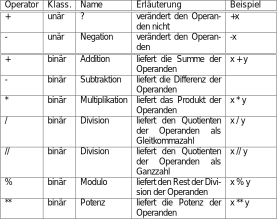
\includegraphics[width=\textwidth]{img/operatoren.pdf}




\par\noindent\textbf{Arithmetische Operatoren}

\begin{verbatim}
>>> x,y = 5,2
>>> +x
5
>>> -x
-5
>>> x + y
7
>>> x - y
3
>>> x * y
10
>>> x / y
2.5
>>> x // y
2
>>> x % y
1
>>> x ** y
25
\end{verbatim}




\par\noindent\textbf{Logische Operatoren}

\begin{itemize}
\itemsep1pt\parskip0pt\parsep0pt
\item
  {Die logischen Operatoren dienen dem Verarbeiten von Wahrheitswerten.}
\item
  {Jeder Wert bekommt in Python automatisch einen Wahrheitswert
  zugewiesen (\textbf{True} oder \textbf{False}).}
\item
  {Die Wahrheitswerte werden dem Datentyp \emph{bool} zugeschrieben.}
\item
  {Negative Zahlen einschließlich der Zahl \$0\$ besitzen den
  Wahrheitswert \textbf{False}.}
\item
  {Alle ``leeren'' Werte (der leere String \texttt{""} oder die leere
  Liste \texttt{{[}{]}}) besitzen ebenfalls den Wahrheitswert
  \textbf{False}.}
\item
  {Die logischen Operatoren prüfen den Wahrheitswert von Werten und
  liefern als Ergebnis einen Wahrheitswert zurück.}
\end{itemize}




\par\noindent\textbf{Logische Operatoren}

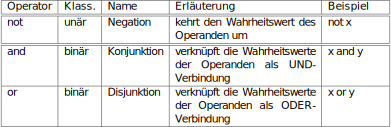
\includegraphics[width=\textwidth]{img/logische_operatoren.pdf}




\par\noindent\textbf{Logische Operatoren}

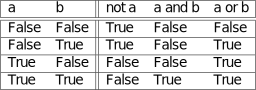
\includegraphics[width=\textwidth]{img/truth_table.pdf}




\par\noindent\textbf{Logische Operatoren}

Wenn andere Werte als der Datentyp \emph{bool} mit den Operatoren
\par\noindent\textbf{and} und \textbf{or} verknüpft werden, so wird immer einer der
beiden Operanden zurückgegeben, wobei die Bedingungen für die Rückgabe
wie folgt sind:

\begin{itemize}
\itemsep1pt\parskip0pt\parsep0pt
\item
  {{[}\textbf{and}{]}}

  \begin{itemize}
  \itemsep1pt\parskip0pt\parsep0pt
  \item
    {Wenn der erste Operand falsch ist, wird dieser zurückgegeben.}
  \item
    {Wenn der erste Operand wahr ist, wird der zweite Operand
    zurückgegeben.}
  \end{itemize}
\item
  {{[}\textbf{or}{]}}

  \begin{itemize}
  \itemsep1pt\parskip0pt\parsep0pt
  \item
    {Wenn der erste Operand wahr ist, wird dieser zurückgegeben.}
  \item
    {Wenn der erste Operand falsch ist, wird der zweite Operand
    zurückgegeben.}
  \end{itemize}
\end{itemize}




\par\noindent\textbf{Logische Operatoren}

\begin{verbatim}
>>> x,y = True,False
>>> not x
False
>>> not y
True
>>> x and y
False
>>> x or y
True
>>> x,y = False,False
>>> not x and not y
True
>>> x and y
False
>>> x or y
False
>>> x,y = 'harry','potter'
>>> x and y
'potter'
>>> x or y
'harry'
>>> x = False
>>> x and y
False
>>> x or y
'potter'
\end{verbatim}




\par\noindent\textbf{Relationale Operatoren}

\begin{itemize}
\itemsep1pt\parskip0pt\parsep0pt
\item
  {Relationale Operatoren liefern immer einen Wahrheitswert in Bezug auf
  die Relation zurück, die überprüft werden soll.}
\item
  {Bei den relationalen Operatoren kann zwischen Vergleichs-, Element-
  und Identitätsoperatoren unterschieden werden.}

  \begin{itemize}
  \itemsep1pt\parskip0pt\parsep0pt
  \item
    {Vergleichsoperatoren dienen dem Vergleich von Operanden
    hinsichtlich ihrer Werte.}
  \item
    {Zugehörigkeitsoperatoren dienen der Ermittlung der Zugehörigkeit
    eines Operanden zu anderen Operanden.}
  \item
    {Identitätsoperatoren dienen der Ermittlung von
    Identitätsverhältnissen, wobei Identität von Gleichheit ähnlich
    abgegrenzt wird wie dies im Deutschen mit Hilfe der Wörter
    \emph{dasselbe} vs. \emph{das gleiche} getan wird.}
  \end{itemize}
\end{itemize}




\par\noindent\textbf{Relationale Operatoren}

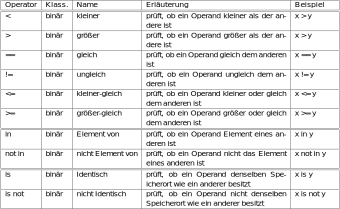
\includegraphics[width=\textwidth]{img/relationale_operatoren.pdf}




\par\noindent\textbf{Relationale Operatoren: Vergleichsoperatoren}

\begin{verbatim}
>>> x,y = 5,10
>>> x > y
False
>>> x < y
True
>>> x == y
False
>>> x != y
True
>>> x <= y
True
>>> x >= y
False
\end{verbatim}




\par\noindent\textbf{Relationale Operatoren: Zugehörigkeitsoperatoren}

\begin{verbatim}
>>> x,y = 'doculect','cul'
>>> x in y
False
>>> y in x
True
>>> x not in y
True
\end{verbatim}




\par\noindent\textbf{Relationale Operatoren: Identitätsoperatoren}

\begin{verbatim}
>>> x = 1,2
>>> y = x
>>> x is y
True
>>> y = 1,2
>>> x is y
False
\end{verbatim}




\par\noindent\textbf{Arithmetische Operatoren}

Die arithmetischen Operatoren in JavaScript sind im Großen und Ganzen
identisch mit denen in Python. Lediglich der Potenz-Operator \texttt{**}
existiert nicht.




\par\noindent\textbf{Arithmetische Operatoren}

\begin{verbatim}
> var x = 5; var y = 2;
> +x;
5
> -x;
-5
> x + y;
7
> x - y;
3
> x * y;
10
> x / y;
2.5
> x // y;
2
> x % y;
1
> Math.pow(x,y); // x ** y in Python
25
\end{verbatim}




\par\noindent\textbf{Logische Operatoren}

Funktionell sind die logischen Operatoren in JavaScript identisch mit
denen in Python, jedoch werden an Stelle der Schlüsselwörter
\par\noindent\textbf{and}, \textbf{or} und \textbf{not} in JavaScript die Zeichen
\par\noindent\textbf{\textbackslash{}\&\textbackslash{}\&},
\par\noindent\textbf{\textbar{}\textbar{}} und \textbf{!} verwendet. Ferner werden
die beiden Werte des Datentyps \textbf{bool} klein geschrieben
(\textbf{true} und \textbf{false} anstelle von \textbf{True} und
\par\noindent\textbf{False}).




\par\noindent\textbf{Logische Operatoren}

\begin{verbatim}
> var x = true; var y = false
> !x; // not x in Python
false
> !y // not y in Python
true
> x && y // x and y in Python
false
> x || y // x or y in Python
true
> var x = false; var y = false;
> ! x && ! y // not x and not y in Python
true
> x && y
false
> x || y
false
> var x = 'harry'; var y = 'potter';
> x && y
'potter'
> x || y
'harry'
> var x = False
> var x && y
false
>>> x || y
'potter'
\end{verbatim}




\par\noindent\textbf{Relationale Operatoren}

Auch die relationalen Operatoren in JavaScript sind denen in Python sehr
ähnlich. Es fehlen jedoch die Operatoren \textbf{in} und \textbf{not
in}. Anstelle der Schlüsselwörter \textbf{is} und \textbf{is not} werden
die Symbole \textbf{===} und \textbf{!==} verwendet.




\par\noindent\textbf{Relationale Operatoren: Vergleichsoperatoren}

\begin{verbatim}
> var x = 5; var y = 10;
> x > y
false
> x < y
true
> x == y
false
> x != y
true
> x <= y
true
> x >= y
false
\end{verbatim}




\par\noindent\textbf{Relationale Operatoren: Vergleichsoperatoren}

\begin{verbatim}
> var x = 'doculect'; var y = 'cul';
> y.indexOf(x) != -1 // x in y in Python
false
> x.indexOf(y) != -1 // y in x in Python
true
> y.indexOf(x) == -1 // x not in y in Python
true
\end{verbatim}




\par\noindent\textbf{Relationale Operatoren: Vergleichsoperatoren}

\begin{verbatim}
> var x = [1, 2] // x = [1,2] in Python
> var y = x
> x === y // x is y in Python
true
> y = [1, 2] 
> x === y // x is y in Python
false
\end{verbatim}

\subsection{Kontrollstrukturen}

\subsubsection{Allgemeines}
\par\noindent\textbf{\href{http://de.wikipedia.org/wiki/Kontrollstruktur}{Gängige
Begriffserklärung aus Wikipedia}}

\begin{quote}
Kontrollstrukturen (Steuerkonstrukte) werden in imperativen
Programmiersprachen verwendet, um den Ablauf eines Computerprogramms zu
steuern. Eine Kontrollstruktur gehört entweder zur Gruppe der
Verzweigungen oder der Schleifen. Meist wird ihre Ausführung über
logische Ausdrücke der booleschen Algebra beeinflusst.
\end{quote}



\par\noindent\textbf{Begriffserklärung in
\href{http://bibliography.lingpy.org?key=Weigend2008}{Weigend
(2008:127)}}

\begin{quote}
Kontrollstrukturen legen fest, in welcher Reihenfolge und unter welchen
Bedingungen die Anweisungen eines Programms abgearbeitet werden.
\end{quote}



\par\noindent\textbf{Typen von Kontrollstrukturen}

\begin{itemize}
\itemsep1pt\parskip0pt\parsep0pt
\item
  {\textbf{Verzweigungen} kontrollieren den Fluss eines Programms, indem
  sie dieses, abhängig von bestimmten Gegebenheiten, in unterschiedliche
  Bahnen lenken}
\item
  {\textbf{Schleifen} kontrollieren den Fluss eines Programms, indem sie
  Operationen wiederholt auf Objekte anwenden}
\end{itemize}



\par\noindent\textbf{Typen von Kontrollstrukturen}

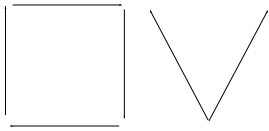
\includegraphics[width=\textwidth]{img/kontrollstrukturen.pdf}


\subsubsection{\ldots in Python}

\par\noindent\textbf{Allgemeines}

\begin{itemize}
\itemsep1pt\parskip0pt\parsep0pt
\item
  {Python kennt insgesamt vier verschiedene Kontrollstrukturen: zwei
  Verzweigungsstrukturen (\textbf{if}, \textbf{try}) und zwei
  Schleifenstrukturen (\textbf{for}, \textbf{while}).}
\item
  {Das besondere an den Kontrollstrukturen in Python ist deren enge
  Anbindung an logische Ausdrücke, welche einen sehr kompakten, sehr
  leicht verständlichen Kode erlauben.}
\end{itemize}


\par\noindent\textbf{Verzweigungen: if, elif, und else}

\begin{itemize}
\itemsep1pt\parskip0pt\parsep0pt
\item
  {Bei der \textbf{if}-Verzweigung wird ein Programmabschnitt unter
  einer bestimmten Bedingung ausgeführt.}
\item
  {Dabei wird eine Bedingung auf ihren Wahrheitswert getestet. Trifft
  sie zu, wird das Programm entsprechend weitergeführt. Trifft sie nicht
  zu, unterbleibt der Abschnitt.}
\item
  {Es können auch mehrere Bedingungen auf ihren Wahrheitswert überprüft
  und entsprechend mehrere verschiedene Programmabschnitte aktiviert
  werden.}
\item
  {Es gibt in Python auch die Möglichkeit, \emph{nichts} zu tun, wenn
  eine Bedingung zutrifft. Dies muss durch das Schlüsselwort
  \textbf{pass} festgelegt werden.}
\end{itemize}



\par\noindent\textbf{Verzweigungen: if, elif, und else}

\begin{verbatim}
>>> x, y, yes, no = 10, 0, "yes", "no"
>>> if x: print(yes)
yes
>>> if y: print(yes)
>>> if not x: print(yes)
    elif not y: print no
no
>>> if 1 > 10: print("Eins ist groesser als zehn.")
    elif 1 < 10: print("Eins ist kleiner als zehn.")
Eins ist kleiner als zehn.
>>> if x or y: print("Einer von beiden Werten ist wahr.")
    else: print("Keiner von beiden Werten ist wahr.")
Einer von beiden Werten ist wahr.
>>> if x == 10: pass
    else: print("Danke, Herr Jauch!")
\end{verbatim}


\par\noindent\textbf{Verzweigungen: try und except}

\begin{itemize}
\itemsep1pt\parskip0pt\parsep0pt
\item
  {Eine sehr wichtige und nützliche Verzweigunsstruktur bietet Python
  mit \textbf{try} und \textbf{except}.}
\item
  {Hierbei wird nicht eine Bedingung auf ihren Wahrheitswert überprüft,
  sondern getestet, ob ein Statement eine Fehlermeldung hervorruft.}
\item
  {Auf diese Weise kann man gezielt auf mögliche Fehler reagieren.}
\item
  {Fehler können dabei gezielt entsprechend ihrer Klasse eingeordnet
  werden.}
\item
  {Auf diese Weise können gezielt bestimmte Fehler angesprochen werden,
  die vom Programm ignoriert werden sollen.}
\end{itemize}



\par\noindent\textbf{Verzweigungen: try und except}

\begin{verbatim}
>>> try: x = int(input())
    except: print("Der Wert, den Sie eingegeben haben, ist kein Integer!")
2
>>> try: x = int(input())
    except ValueError: print("Der Wert, den Sie eingegeben haben, ist kein Integer!")
2.0
Der Wert, den Sie eingegeben haben, ist kein Integer!"
>>> x = input()
10
>>> x, y = 10, 0 
>>> try: x / y
    except ZeroDivisionError: print("Durch Null kann man nicht teilen!")
Durch Null kann man nicht teilen.
>>> try: x = int(input())
    except ValueError: print("Falscher Wert für Integer!")
10.0
Falscher Wert für Integer!
\end{verbatim}


\par\noindent\textbf{Schleifen: while}

\begin{itemize}
\itemsep1pt\parskip0pt\parsep0pt
\item
  {Mit Hilfe von Schleifenkonstruktionen werden Blöcke von Anweisungen
  in Programmen wiederholt ausgeführt, bis eine Abbruchsbedingung
  eintritt, bzw. so lange eine Bedingung zutrifft.}
\item
  {Wie für Verzweigunsstrukturen werden auch die Bedingungen in
  Schleifen auf Grundlage der Auswertung von Wahrheitswerten errechnet.}
\item
  {Der Abbruch einer Schleife kann in Python bewusst durch das
  Schlüsselwort \textbf{break} gesteuert werden.}
\end{itemize}




\par\noindent\textbf{Schleifen: while}

\begin{verbatim}
>>> a = 10
>>> while a > 0: 
        print(a," ist groesser als 0.")
        a -= 1 # wir lassen der Wert gegen 0 laufen

10 ist groesser als 0
9 ist groesser als 0
8 ist groesser als 0
7 ist groesser als 0
6 ist groesser als 0
5 ist groesser als 0
4 ist groesser als 0
3 ist groesser als 0
2 ist groesser als 0
1 ist groesser als 0
>>> while True:
        b = input("Sag was: ")
        print b
        if not b:
            print("Aaaaaabbbbbrrrrruuuuccccccch!")
            break
Sag was: bla
bla
Sag was: bloed
bloed
Aaaaaabbbbbrrrrruuuuccccccch!
\end{verbatim}




\par\noindent\textbf{Schleifen: for}

\begin{itemize}
\itemsep1pt\parskip0pt\parsep0pt
\item
  {Während bei der \textbf{while}-Schleife die Abbruchsbedingung immer
  explizit genannt werden muss, gilt dies nicht für die
  \textbf{for}-Schleife.}
\item
  {Hier wird explizit und im Voraus festgelegt, wie oft, bzw. in Bezug
  auf welche Objekte eine bestimmte Operation ausgeführt werden soll,
  weshalb sich die \textbf{for}-Schleife anbietet, wenn man die Anzahl
  der Operationen kennt, die man durchführen will.}
\item
  {Der Bereich, in dem in Python eine Operation mit Hilfe der
  \textbf{for}-Schleife ausgeführt wird, wird zumeist mit Hilfe der
  Funktion \textbf{range()} angegeben, welche automatisch eine Liste von
  Integern erzeugt, über die dann iteriert wird.}
\end{itemize}




\par\noindent\textbf{Schleifen: for}

\begin{verbatim}
>>> a = range(5)
>>> a
range(0,5)
>>> list(a)
[0, 1, 2, 3, 4]
>>> for i in range(5): print(i)
0
1
2
3
4
>>> einkaufsliste = ['mehl','butter','zitronen','bier']
>>> for element in einkaufsliste: print element
mehl
butter
zitronen
bier
>>> namen = ['peter','frank','karl','jan']
>>> for name in namen: print(name)
peter
frank
karl
jan
>>> woerter = ['haus','kaffee','getraenk','wasser','flasche']
>>> for wort in woerter: print(wort)
haus
kaffee
getraenk
wasser
flasche
\end{verbatim}


\subsubsection{\ldots{} in JavaScript}

\par\noindent\textbf{Verzweigungen: if, else if und else}

Die if-else-Verzweigung in JavaScript unterscheidet sich in ihrer Syntax
von Python, nicht jedoch in der grundlegenden Konzeption, auf der sie
aufbaut. Auch in JavaScript wird der Wahrheitswert einer Datenstruktur
getestet und entsprechend reagiert. Anstelle von ``elif'' wird dabei in
javaScript ``else if'' geschrieben. Ferner werden hässliche Klammern
verwendet anstelle der schönen Einrückungen, die in Python verwendet
werden.




\par\noindent\textbf{Verzweigungen: if, else if und else}

\begin{verbatim}
> var x = 10; var y = 0; var yes = 'yes'; var no = 'no';
> if (x) {console.log(yes);} // if x: print(yes) in Python
yes
> if (y) {console.log(yes);} // if y: print(yes) in Python 
>>> if (!x) {console.log(yes);}
    else if(!y) { console.log(no);}
no
>>> if (1 > 10) {console.log("Eins ist groesser als zehn.");}
    else if (1 < 10) {console.log("Eins ist kleiner als zehn.");}
Eins ist kleiner als zehn.
>>> if (x || y) {console.log("Einer von beiden Werten ist wahr.");} // if x or y in Python
    else {console.log("Keiner von beiden Werten ist wahr.");}
Einer von beiden Werten ist wahr.
>>> if (x == 10) {}
    else {console.log("Danke, Herr Jauch!");}
\end{verbatim}




\par\noindent\textbf{Verzweigungen: try und catch}

Anstelle von \textbf{try} und \textbf{except} bietet JavaScript die
Verzweigung \textbf{try} und \textbf{catch} an. Die Syntax ist auch hier
wieder anders als in Python, die grundlegende Struktur ist jedoch sehr
ähnlich. Allerdings sollte man diese Verzweigung nach Möglichkeit nur
spärlich anwenden, da eine Vielzahl von Fehlern in JavaScript nicht als
solche definiert werden. So führt eine Division durch 0 beispielsweise
nicht zu einem ZeroDivisionError, sondern zum Wert \emph{Infinity}.
Ferner führt der Befehl
\texttt{parseInt(\textquotesingle{}m\textquotesingle{})} nicht zu einem
ValueError, sondern zum Wert \emph{NaN}. Aus diesem Grund werden
\par\noindent\textbf{try} und \textbf{catch} hier nicht weiter behandelt.




\par\noindent\textbf{Schleifen: while}

Abgesehen von der Verwendung der hässlichen Klammerstrukturen
funktioniert die \textbf{while}-Schleife in JavaScript im Prinzip
genauso wie die \textbf{while}-Schleife in Python. Auch das
Schlüsselwort \textbf{break} kann verwendet werden.




\par\noindent\textbf{Schleifen: while}

\begin{verbatim}
> var a = 10
> while (a > 0) { console.log(a+" ist groesser als 0."); a -= 1;}
10 ist groesser als 0
9 ist groesser als 0
8 ist groesser als 0
7 ist groesser als 0
6 ist groesser als 0
5 ist groesser als 0
4 ist groesser als 0
3 ist groesser als 0
2 ist groesser als 0
1 ist groesser als 0
> var a = 10;
> while(true){a -= 1; console.log(a+' ist groesser als 0'); if(a == 0){break;}}
9 ist groesser als 0 
8 ist groesser als 0 
7 ist groesser als 0 
6 ist groesser als 0 
5 ist groesser als 0 
4 ist groesser als 0 
3 ist groesser als 0 
2 ist groesser als 0 
1 ist groesser als 0 
0 ist groesser als 0 
\end{verbatim}




\par\noindent\textbf{Schleifen: for}

In Bezug auf die \textbf{for}-Schleife unterscheiden sich Python und
JavaScript ein wenig mehr als in Bezug auf die anderen
Kontrollstrukturen. Während die \textbf{for}-Schleife in Python generell
auf der Datenstruktur von iterierbaren Elementen (vorrangig Listen)
aufbaut, wird in JavaScript eine explizite Zählerstruktur benötigt. Zwar
gibt es auch ein \textbf{for value in iterable}-Konstrukt in JavaScript,
jedoch gibt dies nur die Schlüsselwerte von Objekten
(\textbf{dictionaries} in Python) aus und sollte nie zusammen mit Arrays
verwendet werden.




\par\noindent\textbf{Schleifen: for}

\begin{verbatim}
> var liste = ["a", "b", "c", "d"];
> for (var i=0; i < liste.length; i++) {console.log(i, liste[i]);}
0 'a'
1 'b'
2 'c'
3 'd'
> for (var i=0,elm; elm=liste[i]; i++) {console.log(i, elm);}
0 'a'
1 'b'
2 'c'
3 'd'
> var myobj = {"a":1, "b":2, "c":3, "d":4};
> for (key in myobj) {console.log(key, myobj[key]);}
a 1
b 2
c 3
d 4
\end{verbatim}


\section{Funktion}
\hyperdef{}{tilda}{}

\subsection{Funktionen im Allgemeinen}

\subsubsection{\texorpdfstring{{Begriffserklärung}}{Begriffserklärung}}

\par\noindent\textbf{\href{http://de.wikipedia.org/wiki/Funktion\%20(Mathematik)}{Funktionen
in der Mathematik (laut Wikipedia)}}

\begin{quote}
In der Mathematik ist eine Funktion oder Abbildung eine Beziehung
zwischen zwei Mengen, die jedem Element der einen Menge
(Funktionsargument, unabhängige Variable, x-Wert) genau ein Element der
anderen Menge (Funktionswert, abhängige Variable, y-Wert) zuordnet. Das
Konzept der Funktion oder Abbildung nimmt in der modernen Mathematik
eine zentrale Stellung ein; es enthält als Spezialfälle unter anderem
parametrische Kurven, Skalar- und Vektorfelder, Transformationen,
Operationen, Operatoren und vieles mehr.
\end{quote}



\par\noindent\textbf{\href{http://de.wikipedia.org/wiki/Funktion\%20(Programmierung)}{Funktionen
in der Programmierung (laut Wikipedia)}}

\begin{quote}
Eine Funktion (engl.: function, subroutine) ist in der Informatik die
Bezeichnung eines Programmierkonzeptes, das große Ähnlichkeit zum
Konzept der Prozedur hat. Hauptmerkmal einer Funktion ist es, dass sie
ein Resultat zurückliefert und deshalb im Inneren von Ausdrücken
verwendet werden kann. Durch diese Eigenschaft grenzt sie sich von einer
Prozedur ab, die nach ihrem Aufruf kein Ergebnis/Resultat zurück
liefert. Die genaue Bezeichnung und Details ihrer Ausprägung ist in
verschiedenen Programmiersprachen durchaus unterschiedlich.
\end{quote}



\subsubsection{\texorpdfstring{{Typen von
Funktionen}}{Typen von Funktionen}}

Da entscheidend für Funktionen der Eingabewert und der Rückgabewert
sind, können wir ganz grob die folgenden speziellen Typen von Funktionen
identifizieren:

\begin{itemize}
\itemsep1pt\parskip0pt\parsep0pt
\item
  {Funktionen ohne Rückgabewert (Prozedur)}
\item
  {Funktionen ohne Eingabewert}
\item
  {Funktionen mit einer festen Anzahl von Eingabewerten}
\item
  {Funktionen mit einer beliebigen Anzahl von Eingabewerten}
\end{itemize}
i
\subsection{Funktionen in Python}


\par\noindent\textbf{Vorweg}

In Python sind Funktionen spezielle Datentypen. Sie unterscheiden sich
von anderen Datentypen wie \textbf{strings} oder \textbf{integers}
dadurch, dass sie zusätzlich aufgerufen werden können (\emph{callable
types}).



\subsubsection{Grundlagen}

\par\noindent\textbf{Allgemeine Struktur}

\begin{verbatim}
def functionName(
        parameterA,
        ...,
        keywordA='defaultA',
        ...,
        ):
    """
    docString
    """
    functionBody
    return functionValue
\end{verbatim}




\par\noindent\textbf{Erstes Beispiel}

\begin{verbatim}
def stoneAgeCalculator(intA, intB, calc='+'):
    """
    This is the famous stoneAgeCalculator, a program written by the very first
    men on earth who brought the fire to us and were the first to dance naked
    on the first of May.
    """
    # check for inconsistencies in the input for keyword calc
    if calc not in ['+', '-', '*', '/']:
        raise ValueError('The operation you chose is not defined.')

    # start the calculation, catch errors from input with a simple
    # try-except-structure
    try:
        if calc == '+':
            return intA + intB
        elif calc == '-':
            return intA - intB
        elif calc == '*':
            return intA * intB
        else:
            return intA / intB
    except:
        raise ValueError('No way to operate on your input.')
\end{verbatim}




\par\noindent\textbf{Aufrufen und Ausführen}

\begin{quote}
Eine Funktion wird aufgerufen, indem der Name der Funktion angegeben
wird, gefolgt von einer Liste aktueller Parameter in Klammern.
\href{http://bibliography.lingpy.org?key=Weigend2008}{(Weigend
2008:144)}
\end{quote}

\begin{verbatim}
>>> a = range(5)
>>> a = int('1')
>>> range(5)
range(0,5)
>>> int('1')
1
>>> float(1)
1.0
>>> print('Hallo Welt!')
Hallo Welt!
>>> list('hallo')
['h', 'a', 'l', 'l', 'o']
\end{verbatim}




\par\noindent\textbf{Die Funktionsdokumentation}

Für jede Funktion, die in Python definiert wird, steht eine automatische
Dokumentation bereit, welche mit Hilfe der Parameter und der Angaben im
Docstring generiert wird. Die Dokumentation einer Funktion wird mit
Hilfe von \texttt{help(function)} aufgerufen. Mit Hilfe der
Funktionsdokumentation lässt sich leicht ermitteln, welche Eingabewerte
eine Funktion benötigt, wie sie verwendet wird, und welche Werte sie
zurückliefert. Docstrings lassen sich am besten interaktiv einsehen.



\subsubsection{Parameter und Schlüsselwörter}

\par\noindent\textbf{Parameter}

Mit Hilfe von Funktionen werden Eingabewerte (Parameter) in Ausgabewerte
umgewandelt. Bezüglich der Datentypen von Eingabewerten gibt es in
Python keine Grenzen. Alle Datentypen (also auch Funktionen selbst)
können daher als Eingabewerte für Funktionen verwendet werden.
Gleichzeitig ist es möglich, Funktionen ohne Eingabewerte oder ohne
Ausgabewerte zu definieren. Will man eine beliebige Anzahl an Parametern
als Eingabe einer Funktion verwenden, so erreicht man dies, indem man
der Parameterbezeichnung einen Stern (*) voranstellt. Die Parameter von
Eingabeseite werden innerhalb der Funktion dann automatisch in eine
Liste umgewandelt, auf die mit den normalen Listenoperationen
zugegriffen werden kann.




\par\noindent\textbf{Parameter}

\begin{verbatim}
>>> def leer():
...     print "leer"
>>> def empty():
...     pass
>>> def gruss1(wort):
...     print wort
>>> def gruss2(wort):
...     return wort
>>> def eins():
...     """Gibt die Zahl 1 aus."""
...     return 1
>>> leer()
leer
>>> empty
... 
>>> empty()
>>> type(empty)

>>> a = eins()
>>> a
1
>>> print bla.func_doc
Gibt die Zahl 1 aus.
>>> def printWords(\*words):
...     for word in words:
...         print(word)
...
>>> printWords('mama','papa','oma',opa')
mama
papa
oma
opa
\end{verbatim}




\par\noindent\textbf{Schlüsselwörter}

Als Schlüsselwörter bezeichnet man Funktionsparameter, die mit einem
Standardwert belegt sind. Werden diese beim Funktionsaufruf nicht
angegeben, gibt es keine Fehlermeldung, sondern anstelle der fehlenden
Werte wird einfach auf den Standardwert zurückgegriffen. Gleichzeitig
braucht man beim Aufrufen nicht auf die Reihenfolge der Parameter zu
achten, da diese ja durch die Anbindung der Schlüsselwörter vordefiniert
ist. Weist eine Funktion hingegen Schlüsselwörter und Parameter auf, so
müssen die Parameter den Schlüsselwörtern immer vorangehen.




\par\noindent\textbf{Schlüsselwörter}

\begin{verbatim}
>>> def wind(country, season='summer')
...     """Return the typical wind conditions for a given country."""
...     if country == "Germany" and season == 'summer':
...         print("There's strong wind in",country)
...     else:
...         print("This part hasn't been programmed yet.")
...
>>> wind('Germany'):
There's strong wind in Germany.
>>> wind('Germany,season='winter')
This part hasn't been programmed yet.
\end{verbatim}



\subsubsection{\texorpdfstring{{Spezialfälle}}{Spezialfälle}}

\par\noindent\textbf{Prozeduren}

\begin{quote}
Prozeduren sind Funktionen, die den Wert \textbf{None} zurückgeben.
Fehlt in einer Funktionsdefinition die \textbf{return}-Anweisung, wird
automatisch der Wert \textbf{None} zurückgegeben.
\href{http://bibliography.lingpy.org?key=Weigend2008}{(Weigend 2008:
155)}
\end{quote}

\begin{verbatim}
>>> def quak(frosch=''):
...     print("quak")
...
>>> quak()
quak
>>> a = quak()
quak
>>> type(a)
\end{verbatim}



\par\noindent\textbf{Rekursive Funktionen}

\begin{quote}
Rekursive Funktionen sind solche, die sich selbst aufrufen.
\href{http://bibliography.lingpy.org?key=Weigend2008}{(Weigend 2008:
151)}
\end{quote}

\begin{verbatim}
>>> def factorial(number):
...     """
...     Aus: http://www.dreamincode.net/code/snippet2800.htm
...     """
...     if number == 0:
...         return 1
...     else:
...         value = factorial(n-1)
...         result = n * value
...         return result
...
>>> factorial(4)
24
\end{verbatim}



\par\noindent\textbf{Globale und lokale Variablen}

Es muss bei Funktionen zwischen lokalen und globalen Variablen
unterschieden werden. Lokale Variablen haben nur innerhalb einer
Funktion ihren Gültigkeitsbereich. Globale Variablen hingegen gelten
auch außerhalb der Funktion. Will man mit Hilfe einer Funktion eine
Variable, die global, also außerhalb der Funktion deklariert wurde,
verändern, so muss man ihr das \emph{Keyword} \textbf{global}
voranstellen. Dies sollte man jedoch nach Möglichkeit vermeiden, da dies
schnell zu Fehlern im Programmablauf führen kann. Lokale und globale
Variablen sollten nach Möglichkeit getrennt werden.



\par\noindent\textbf{Globale und lokale Variablen}

\begin{verbatim}
>>> s = 'globaler string'
>>> def f1():
...     print(s)
...
>>> def f2():
...     s = 'lokaler string'
...     print(s)
...
>>> f1()
globaler string
>>> f2()
lokaler string
>>> def f3():
...     global s
...     s = 'lokaler string'
...     print(s)
>>> s = 'globaler string'
>>> f3()
lokaler string
>>> print(s)
lokaler string
\end{verbatim}

\subsection{Funktionen in JavaScript}

\subsubsection{Grundlagen}

\par\noindent\textbf{Allgemeines vorweg}

Wie in Python, so sind auch in JavaScript Funktionen spezielle
Datentypen.

\par\noindent\textbf{Allgemeine Struktur}

\begin{verbatim}
function functionName (
  parameterA,
  parameterB,
  parameterC,
  ...
  ) {

  functionBody;

  return functionValue;
}
\end{verbatim}

\par\noindent\textbf{Erstes Beispiel: Der Steinzeittaschenrechner}

\begin{verbatim}
function stoneAgeCalculator(intA, intB, calc) {
  /* This is a very famous StoneAge Calculator. */

  /* check for active values for type */
  if (typeof calc == 'undefined') {
    calc = "+";
  }
  /* check for correct values for calc */
  else if(["+", "-", "*", "/"].indexOf(calc) == -1) {
    return false;
  }

  /* return the stuff */
  if (calc == '+') {return intA + intB;}
  else if (calc == '-') {return intA - intB;}
  else if (calc == '*') {return intA * intB;}
  else if (calc == '/') {return intA / intB;}
  return false;
}
\end{verbatim}




\par\noindent\textbf{Erstes Beispiel: Der Steinzeittaschenrechner}



\subsubsection{\texorpdfstring{{Parameter und
Schlüsselwörter}}{Parameter und Schlüsselwörter}}

\par\noindent\textbf{Parameter und Schlüsselwörter}

Die Handhabung von Parametern und Schlüsselwörtern ist nicht so leicht
in JavaScript wie in Python. Schlüsselwörter gibt eigentlich gar nicht.
Das heißt leider auch, dass man keine Standardwerte für bestimmte
Parameter annehmen kann, was das Programmieren ein wenig umständlich
macht. Um ähnliche Funktionalitäten wie in Python zu erlangen, behilft
man sich meist mit Ersatzkonstruktionen.




\par\noindent\textbf{Parameter und Schlüsselwörter}

\begin{verbatim}
function wind(country, season) {
  /* Return the typical wind conditions for a country */

  /* carry out type check of season, to set the basic value */
  if (typeof season == "undefined") {
    season = "summer";
  }

  if (country == "Germany" and season == "summer") {
    return "There's strong wind in "+country+".";
  }
  else {
    return "This part hasn't been programmed yet.";
  }
}
\end{verbatim}




\par\noindent\textbf{Parameter und Schlüsselwörter}



\subsubsection{\texorpdfstring{{Spezialfälle}}{Spezialfälle}}

\par\noindent\textbf{Prozeduren und Rekursive Funktionen}

Prozeduren und rekursive Funktionen können in JavaScript genauso
verwendet werden wie in Python. Tendentiell werden sehr viel mehr
Prozeduren in JavaScript verwendet, da das Auslösen von Aktionen mit
Hilfe der HTML-Buttons und der ``onclick''-Anweisung am leichtesten
geregelt werden kann.




\par\noindent\textbf{Globale und lokale Variablen}

JavaScript unterscheidet nicht direkt zwischen globalen und lokalen
Variablen: Alles, was auf einer jeweils höheren Ebene definiert wurde,
kann auch auf einer niedrigeren Ebene verwendet werden und umgekehrt.
Das Schlüsselwort \textbf{var} kann jedoch verwendet werden, um zu
gewährleisten, dass Variablen nur innerhalb ihrer jeweiligen Ebene
Geltung haben. Sicherheitshalber sollte man daher vor jede
Variablendeklaration das Schlüsselwort \textbf{var} setzen.




\par\noindent\textbf{Globale und lokale Variablen}

\begin{verbatim}
> s = 'globaler string'
> function f1(){console.log(s)}
> function f2(){s = 'lokaler string'; console.log(s);}
> f1()
'globaler string'
> f2()
'lokaler string'
> function f3() { var s; s = 'lokaler string'; console.log(s);}
> s = 'globaler string';
> f3()
lokaler string
> s 
globaler string
\end{verbatim}


\section{Sequenzvergleiche in der historischen Linguistik}
\hyperdef{}{tilda}{}

\subsection{\texorpdfstring{{Sprachwandel}}{Sprachwandel}}

\subsubsection{\texorpdfstring{{Sprachen}}{Sprachen}}

\par\noindent\textbf{Der Nordwind und die Sonne und das Problem der Sprachgrenzen}

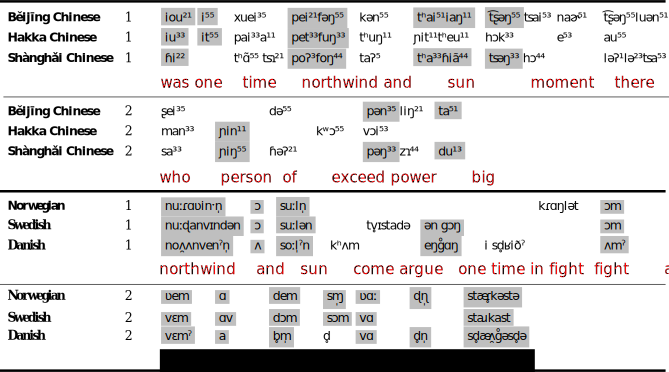
\includegraphics[width=\textwidth]{img/northwind.pdf}

\par\noindent\textbf{Diasysteme}

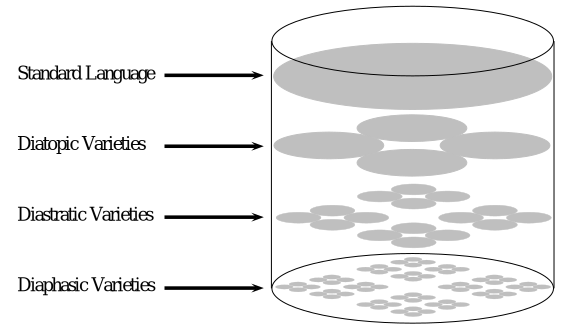
\includegraphics[width=\textwidth]{img/diasystem.pdf}

\par\noindent\textbf{Dimensionen der Sprachvariation}

\includegraphics[width=\textwidth]{img/variation-1.png}

\par\noindent\textbf{Komplexität des Sprachwandels}

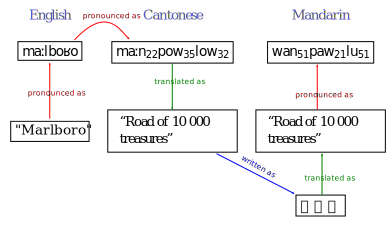
\includegraphics[width=\textwidth]{img/marlboro.pdf}

\subsubsection{\texorpdfstring{{Sprachwandel im
Allgemeinen}}{Sprachwandel im Allgemeinen}}

\par\noindent\textbf{Die komischen Reime in den chinesischen Oden}

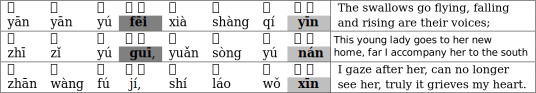
\includegraphics[width=\textwidth]{img/odes.pdf}


\par\noindent\textbf{Die komischen Reime in den chinesischen Oden}

\begin{quote}
The writings of scholars must be made of adequate sounds. Even in the
rural areas everybody orders the sounds harmonically. Can it be that the
ancients solely did not have rhymes? One can say that in the same way in
which ancient times differ from modern times, and places in the North
differ from places in the South, characters change and sounds shift.
This is a natural tendency. Therefore, it is inevitable that reading the
ancient writings with modern pronun- ciation will sound improper and
wrong. (Máoshī Gǔyīnkǎo: 原序, meine Übersetzung)
\end{quote}

\par\noindent\textbf{Wandel als Katastrophe}

Schon früh in der Geschichte der Linguistik war den Forschern in Europa
bewusst, dass Sprachen sich wandeln können. Vorherrschend war dabei
jedoch die Ansicht, dass alle Formen des Wandels ``katastrophisch''
abliefen, dass Wandel also im Rahmen eines unberechenbaren, chaotischen
``Verfalls'' vor sich ginge. Erst spät (zu Beginn des 19. Jahrhunderts)
wurde erstmals klar, dass sich bestimmte Phänomene des Sprachwandels,
insbesondere der Lautwandel, durch eine beachtliche Regelmäßigkeit
auszeichnen.

\par\noindent\textbf{Wandel als Prozess}

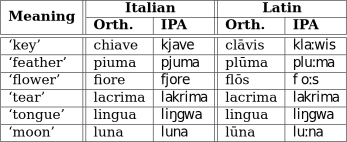
\includegraphics[width=\textwidth]{img/lautwandel-ita-lat.pdf}



\par\noindent\textbf{Wandel und Regelmäßigkeit}

Während den Menschen im Verlaufe der Geschichte bereits relativ lange
bewusst war, dass Sprachen sich ändern können, war es eine radikal neue
Erkenntnis, die sich zu Beginn des 19. Jahrhunderts
herauskristallisierte, dass Sprachen sich in Prozessen ändern, von denen
bestimmte sogar regelmäßig verlaufen können. Mit der Entdeckung der
Regelmäßigkeit einher festigte sich ebenfalls die Erkenntnis, dass
Sprachen miteinander verwandt sein können, wobei Verwandtschaft von
Sprachen dadurch definiert ist, dass miteinander verwandte Sprachen aus
einer gemeinsamen Vorgängersprache entstanden sind, wie bspw. das
Englische und das Deutsche, die beide aus dem Protogermanischen
hervorgegangen sind.


\subsubsection{\texorpdfstring{{Lautwandel}}{Lautwandel}}

\par\noindent\textbf{Wandel als Gesetz
(\href{http://bibliography.lingpy.org?key=Osthoff1878}{Osthoff und
Brugmann 1878: XIII})}

\begin{quote}
Aller lautwandel, soweit er mechanisch vor sich geht, vollzieht sich
nach ausnahmslosen gesetzen, d.h. die richtung der lautbewegung ist bei
allen angehörigen einer sprachgenossenschaft, ausser dem Fall, dass
dialektspaltung eintritt, stets dieselbe, und alle wörter, in denen der
der lautbewegung unterworfene laut unter gleichen verhältnissen
erscheint, werden ohne ausnahme von der änderung ergriffen.
\end{quote}



\par\noindent\textbf{Chaque mot a son histoire}

Nicht alle Linguisten waren der Meinung der Junggrammatiker. Besonders
Dialektologen folgten dem berühmten Slogan \emph{chaque mot a son
histoire} (``jedes Wort hat seine Geschichte''), der gewöhnlich
\href{http://de.wikipedia.org/wiki/Jules_Gilliéron}{Jules Gilliéron
(1854--1926)} zugeschrieben wird
(\href{http://bibliography.lingpy.org?key=Campbell1999}{Campbell 1999:
189}). Die Bedenken der Dialektologen standen jedoch strengenommen nicht
direkt im Widerspruch zur junggrammatischen Doktrin, schließlich besagte
die junggrammatische Theorie ja nicht, dass sich zwangsläufig
\emph{alle} Wörter einer Sprache regelmäßig änderten, sondern lediglich,
dass idiosynkratischer Wandel durch andere Mechanismen (Entlehnung oder
Analogie) erklärt werden konnte
(\href{http://bibliography.lingpy.org?key=Kiparsky1988}{Kiparsky
1988:368}).

\subsection{\texorpdfstring{{Lautwandel}}{Lautwandel}}

\subsubsection{\texorpdfstring{{Mechanismen des
Lautwandels}}{Mechanismen des Lautwandels}}

\par\noindent\textbf{Junggrammatischer Lautwandel (nach
\href{http://bibliography.lingpy.org?key=Wang2006a}{Wang 2006: 109,
meine Übersetzung})}

\begin{quote}
Regarding the lexicon {[}they assumed{]} that a change always affects
the whole lexicon, and can therefore be seen as an abrupt change.
Regarding the sounds {[}they assumed{]} that the change proceeded step
by step, and can therefore be seen as a gradual change.
\end{quote}


\par\noindent\textbf{Lexikalische Diffusion
(\href{http://bibliography.lingpy.org?key=Wang1969}{Wang 1969: 9})}

\begin{quote}
Phonological change may be implemented in a manner that is phonetically
abrupt but lexically gradual. As the change diffuses across the lexicon,
it may not reach all the morphemes to which it is applicable. If there
is another change competing for part of the lexicon, residue may result.
\end{quote}

\par\noindent\textbf{Kompettitierende Theorien der Lautwandelmechanismen}

\tabular{lll}
\includegraphics[width=0.25\textwidth]{img/neo-0.png} &
\includegraphics[width=0.25\textwidth]{img/neo-1.png} &
\includegraphics[width=0.25\textwidth]{img/neo-2.png} \\
\includegraphics[width=0.25\textwidth]{img/neo-3.png} &
\includegraphics[width=0.25\textwidth]{img/neo-4.png} &
\\
\includegraphics[width=0.25\textwidth]{img/diffusion-0.png} &
\includegraphics[width=0.25\textwidth]{img/diffusion-1.png}&
\includegraphics[width=0.25\textwidth]{img/diffusion-2.png}\\
\includegraphics[width=0.25\textwidth]{img/diffusion-3.png}&
\includegraphics[width=0.25\textwidth]{img/diffusion-4.png}&
\\
\endtabular



\par\noindent\textbf{Zwei Mechanismen des Lautwandels
(\href{http://bibliography.lingpy.org?key=Labov1994}{Labov 1994: 471})}

\begin{quote}
There is no basis for contending that lexical diffusion is somehow more
fundamental than regular, phonetically motivated sound change. On the
contrary, if we were to decide the issue by counting cases, there appear
to be far more substantially documented cases of Neogrammarian sound
change than of lexical diffusion.
\end{quote}


\subsubsection{\texorpdfstring{{Typen des
Lautwandels}}{Typen des Lautwandels}}

\par\noindent\textbf{Terminologische Probleme}

Die lange Forschungstradition in der historischen Linguistik hat zur
Postulierung einer Vielzahl unterschiedlicher Typen des Lautwandels\}
geführt. Leider ist die Terminologie, welche verwendet wird, um auf
diese Typen in der Literatur zu verweisen, etwas ``unstetig'' und reicht
von sehr konkreten Termini, welche sehr konkrete Lautwandelinstanzen
abdecken, bis hin zu sehr generellen Termini, die auf den Wandel
abstrakter Lautklassen verweisen.



\par\noindent\textbf{Terminologische Probleme}

Was in der Literatur als \emph{Lautwandeltyp} bezeichnet wird, kann
dabei sowohl das Phänomen des \emph{Rhotazismus} umfassen
(\href{Trask2000}{Trask 2000: 288}), welches, vereinfacht gesagt, einen
Wandel von /s/ nach /r/ bezeichnet, als auch den Prozess der
\emph{Lenisierung}, welcher eine bestimmte Art von Wandel bezeichnet,
``in which a segment becomes less consonant-like than previously''
(\href{Trask2000}{idb. 190}).



\par\noindent\textbf{Definitionen von
\href{http://bibliography.lingpy.org?key=Trask2000}{Trask (2000}}

\begin{itemize}
\itemsep1pt\parskip0pt\parsep0pt
\item
  \textbf{Assimilierung} "Any \textbf{syntagmatic change} in which some
  segment becomes more similar in nature to antother segment int he same
  sequence, usually within a single phonological word or phrase" (30).
\item
  \textbf{Dissimilierung} "Any \textbf{syntagmatic change} in which one
  segment changes so as to become less similar to another segment in the
  same form" (95).
\item
  \textbf{Metathese} "Any \textbf{syntagmatic change} in which the order
  of segments (or simetimes of other phonological elements) in a word is
  altered" (211).
\item
  \textbf{Tonogenese} ``Any process which leads to the introduction of
  tones into a language which formerly lacked them'' (346).
\end{itemize}



\par\noindent\textbf{Definitionen von
\href{http://bibliography.lingpy.org?key=Trask2000}{Trask (2000,
cont.)}}

\begin{itemize}
\itemsep1pt\parskip0pt\parsep0pt
\item
  \textbf{Sandhi} "Any of various phonological processes applying to
  sequences of segments either across morpheme boundaries
  (\emph{internal sandhi}) or across word boundaries (\emph{external
  sandhi})" (296).
\item
  \textbf{Haplologie} ``A type of phonological change (of or
  phonological constraint) in which one of two adjacent syllables of
  identical or similar form is lost (or fails to appear in the first
  place)'' (146).
\item
  \textbf{Elision (Aphaerese, Synkope, Apokope)} "Any of various
  processes in which phonological segments are lost from a word or a
  phrase. Specific varieties of elision are often given special names
  like \textbf{aphaeresis}, \textbf{syncope}, \textbf{apocope,
  synaeresis, synizesis, synaloepha}. Not infrequently this name is
  given to specific processes in particular languages" (102).
\end{itemize}



\par\noindent\textbf{Definitionen von
\href{http://bibliography.lingpy.org?key=Trask2000}{Trask (2000,
cont.)}}

\begin{itemize}
\itemsep1pt\parskip0pt\parsep0pt
\item
  \textbf{Epenthese} ``Any phonological change which inserts a segment
  into a word or form in a position in which no segment was formerly
  present'' (107).
\item
  \textbf{Prothese} "The addition of a segment to the beginning of a
  word. {[}\ldots{}{]} The opposite is \textbf{aphaeresis}" (266).
\item
  \textbf{Nasalierung} ``Any phonological process in which a segment
  acquires a nasal character which it formerly lacked'' (224).
\end{itemize}

\subsubsection{\texorpdfstring{{Typen des
Lautwandels}}{Typen des Lautwandels}}

\par\noindent\textbf{Ein vereinfachtes Modell}

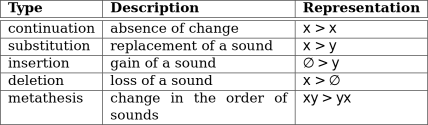
\includegraphics[width=\textwidth]{img/indel.pdf}

\subsection{\texorpdfstring{{Lautwandel}}{Lautwandel}}

\subsubsection{\texorpdfstring{{Typen des
Lautwandels}}{Typen des Lautwandels}}

\par\noindent\textbf{Ein vereinfachtes Modell (Beispiele)}

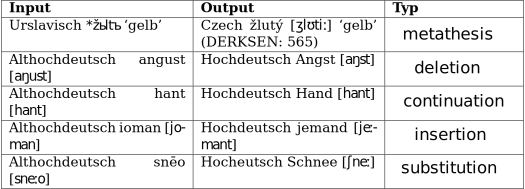
\includegraphics[width=\textwidth]{img/indel-concrete.pdf}


\subsubsection{\texorpdfstring{{Die komparative
Methode}}{Die komparative Methode}}

\par\noindent\textbf{Definitionen}

\href{img/cm-wirr.png}{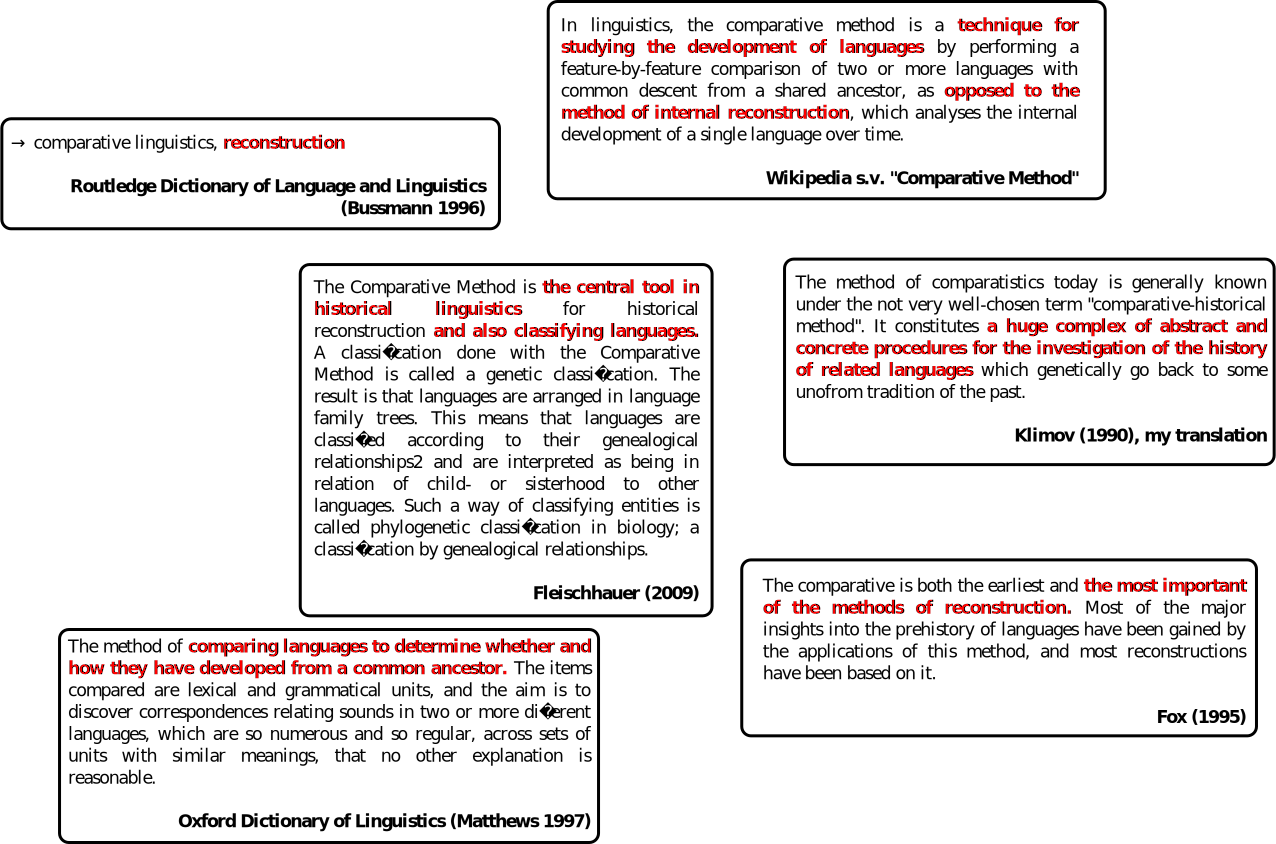
\includegraphics{img/cm-wirr.png}}



\par\noindent\textbf{Ein neuer Definitionsversuch}

Die komparative Methode ist ein Komplex von Verfahren der historischen
Sprachwissenschaft, mit deren Hilfe Sprachen klassifiziert und nicht
belegte Sprachstufen rekonstruiert werden, um somit
Entwicklungsgeschichte von Sprachen zu schreiben. Die Ergebnisse der
komparativen Methoden werden in Form von etymologischen Wörterbüchern,
historischen Grammatiken und Entwicklungsschemata (evolutionäre Bäume
und Netze) kodiert.


\subsubsection{\texorpdfstring{{Die komparative
Methode}}{Die komparative Methode}}

\par\noindent\textbf{Beschreibung des Workflows in
\href{http://bibliography.lingpy.org?key=Ross1996}{Ross und Durie
(1996)}}

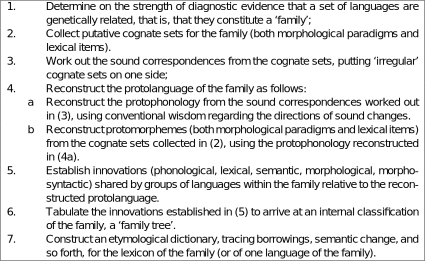
\includegraphics[width=\textwidth]{img/rodu.pdf}



\par\noindent\textbf{Visualisierung des Workflows von
\href{http://bibliography.lingpy.org?key=Ross1996}{Ross und Durie
(1996)}}

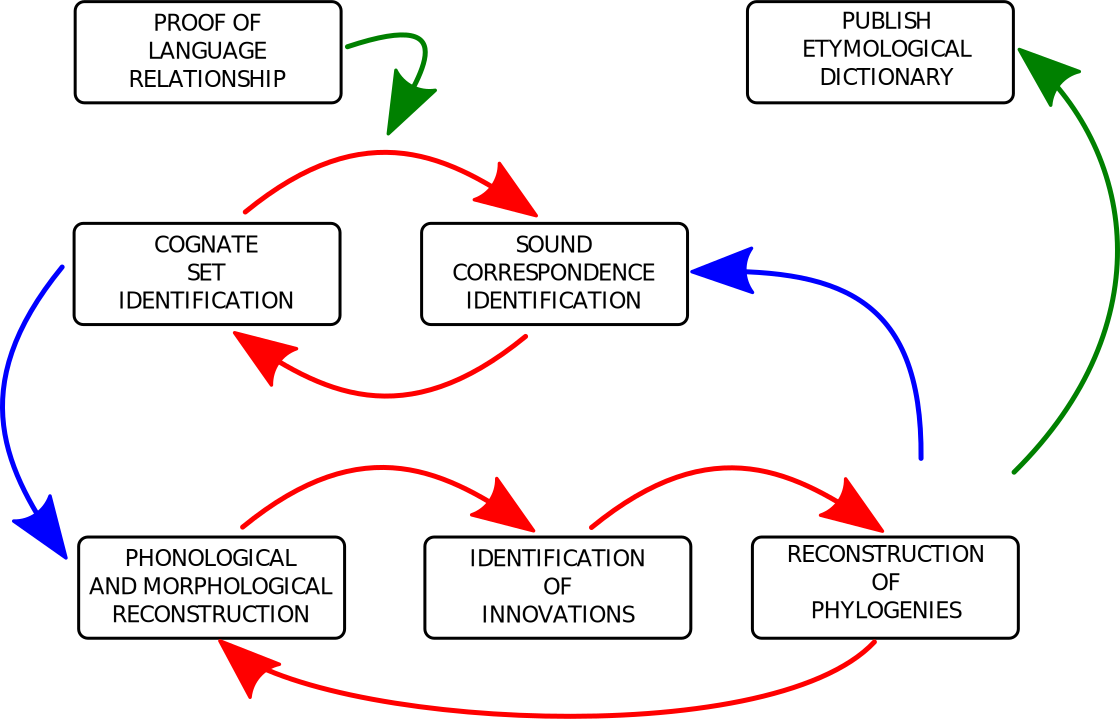
\includegraphics[width=\textwidth]{img/ross-durie-workflow.pdf}



\par\noindent\textbf{Vereinfachter Workflow
\href{http://bibliography.lingpy.org?key=List2014d}{(List 2014)}}

\href{img/cm-simplified.png}{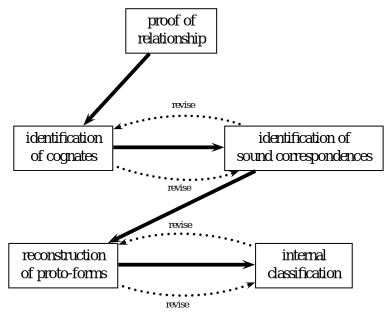
\includegraphics{img/cm-simplified.png}}

\subsection{\texorpdfstring{{Sequenzalinierung}}{Sequenzalinierung}}

\subsubsection{\texorpdfstring{{Sequenzen und
Sequenzvergleiche}}{Sequenzen und Sequenzvergleiche}}

\par\noindent\textbf{Sequenzen: Definition (vgl.
\href{http://bibliography.lingpy.org?key=Boeckenbauer2003}{Böckenbauer
und Bongartz 2003: 30f})}

\par\noindent\textbf{Definition:} Ein \emph{Alphabet} ist eine nicht-leere endliche
Menge deren Elemente \emph{Buchstaben} genannt werden. Eine
\emph{Sequenz} ist eine geordnete Liste von Buchstaben, die aus dem
Alphabet gezogen werden. Die Elemente von Sequenzen werden
\emph{Segmente} genannt, die \emph{Mächtigkeit} einer Sequenz ist die
Anzahl ihrer unterschiedlichen Buchstaben, und die \emph{Länge} einer
Sequenz ist die Anzahl ihrer Segmente.



\par\noindent\textbf{Sequenzen als Perlenketten}

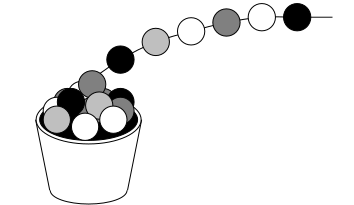
\includegraphics[width=\textwidth]{img/kette.pdf}


\par\noindent\textbf{Vergleich von Sequenzen mit gleicher Länge}

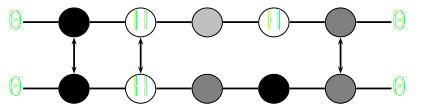
\includegraphics[width=\textwidth]{img/hamming.pdf}



\par\noindent\textbf{Vergleich von Sequenzen mit unterschiedlicher Länge}

\href{img/matchings.png}{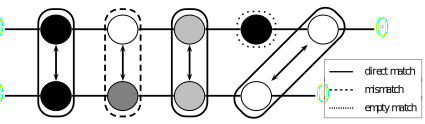
\includegraphics{img/matchings.png}}


\subsubsection{\texorpdfstring{{Alinierung}}{Alinierung}}

\par\noindent\textbf{Definitionsversuch}

\begin{quote}
Eine \emph{Alinierung} von \$n\$ (\$n\textgreater{}1\$) Sequenzen ist
eine \$n\$-reihige Matrix, in der alle Sequenzen dergestalt angeordnet
werden, dass alle matchenden Segmente in derselben Spalte erscheinen,
während nicht-matchende Segmente, die aus leeren Matches resultieren,
durch Gap-Symbole angezeigt werden. (vgl
\href{http://bibliography.lingpy.org?key=Gusfield1997}{Gusfield 1997:
216})
\end{quote}



\par\noindent\textbf{Beispiel}

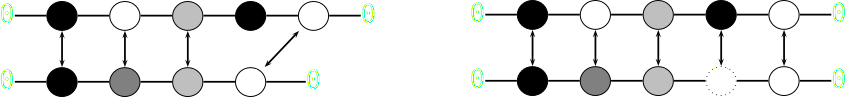
\includegraphics[width=\textwidth]{img/alignment.pdf}



\par\noindent\textbf{Preisfrage}

Die Levenshtein-Distanz zwischen zwei Sequenzen \$S\_1\$ und \$S\_2\$
ist definiert als die Anzahl von Editieroperationen, die notwendig ist,
um \$S₁\$ in \$S\_2\$ zu transformieren. Mit Hilfe des Konzepts der
Alinierung lässt sich dieses Distanzmaß leicht auf die Hamming-Distanz
zurückführen. Wie genau?


\subsubsection{\texorpdfstring{{Phonetische
Alinierung}}{Phonetische Alinierung}}

Obwohl Alinierungsanalysen eine der allgemeinsten Möglichkeiten
darstellen, Sequenzen zu vergleichen, steckt ihre Verwendung in der
historischen Linguistik noch in den Kinderschuhen. Natürlich alinieren
historische Linguisten eigentlich \emph{immer} Wörter und haben dies
auch schon immer getan, da ohne Alinierung überhaupt keine regulären
Lautkorrespondenzen ermittelt werden könnten. Der Sprachvergleich
basierte lange Zeit jedoch eher auf einer impliziten Alinierung, die
selten visualisiert wurde, und wenn doch, dann nur aus illustrativen
Zwecken.



\par\noindent\textbf{Schwierigkeiten der phonetischen Alinierung}

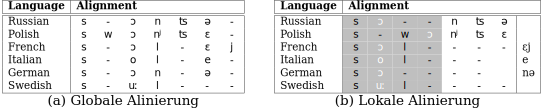
\includegraphics[width=\textwidth]{img/phonalign.pdf}



\par\noindent\textbf{Substantielle und strukturelle Ähnlichkeit}

\begin{itemize}
\itemsep1pt\parskip0pt\parsep0pt
\item
  die Wörter ``schlafen'' und ``Flaschen'' sind recht ähnlich
\item
  die Wörter ``Obst'' und ``Post'' auch
\item
  die Wörter ``Kerker'' und ``Tanten'' sind sich auch recht ähnlich,
  aber auf andere Art und Weise
\end{itemize}

\par\noindent\textbf{Die beiden unterschiedlichen Formen von Ähnlichkeit können wir
``substantielle'' vs. ``strukturelle'' Ähnlichkeit nennen.}



\par\noindent\textbf{Heuristiken für strukturelle Ähnlichkeiten}

Beim Alinieren in der historischen Linguistik ist es wichtig, der
Tatsache Rechnung zu tragen, dass substantielle Ähnlichkeit zwischen
Lauten nicht notwendigerweise auch auf deren Kognazität hinweist. Nur,
wenn zwei Segmente auch systematisch (also in den Sprachsystemen)
korrespondieren, sollten sie tatsächlich als ähnlich angesehen werden.
In den Schritten des Sprachvergleichs kann diese systematische
Ähnlichkeit jedoch schwer ermittelt werden, denn zu Beginn eines
Sprachvergleichs sind weder die kognaten Wörter bekannt, noch die
regulär korrespondierenden Laute.



\par\noindent\textbf{Dolgopolskys Lautklassen}

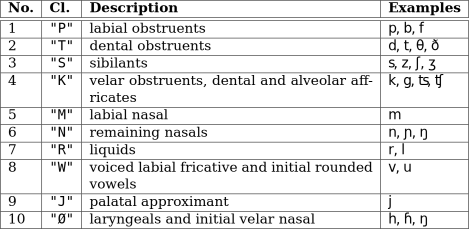
\includegraphics[width=\textwidth]{img/dolgopolsky.pdf}


\section{Sequenzalinierung in JavaScript}
\hyperdef{}{tilda}{}

\subsection{Automatische Sequenzalinierung}

\subsubsection{\texorpdfstring{{Das Problem}}{Das Problem}}

\par\noindent\textbf{Wir wollen zwei Sequenzen automatisch alinieren, aber wie?}

\begin{itemize}
\itemsep1pt\parskip0pt\parsep0pt
\item
  {Eine einfache automatische Lösung wäre es, einfach alle verschiedenen
  Kombinationen durchzutesten.}
\item
  {In einem weiteren Schritt könnten wir dann alle Alinierungen testen
  und ihren ``Score'' berechnen, also sie bewerten, indem wir, zum
  Beispiel, zählen, wie viele Mismatches und leere Matches sie
  aufweisen.}
\item
  {Dann könnten wir den Score für jedes Paar aufsummieren und würden
  einfach die Alinierung mit dem besten Score nehmen.}
\end{itemize}




\par\noindent\textbf{Leider dauert das zu lange!}

Die Zahl aller Möglichen Alinierungen zwischen zwei Strings hängt von
deren Länge ab: Es gilt:

\$N = \textbackslash{}sum\_\{k=0\}\^{}\{\textbackslash{}min(m,n)\}
2\^{}\{k\} \textbackslash{}cdot \textbackslash{}binom\{m\}\{k\}
\textbackslash{}cdot \textbackslash{}binom\{n\}\{k\}\$,

für zwei Strings der Länge \$m\$ und \$n\$.




\par\noindent\textbf{Und was soll das heißen?}

Das wir für die Alinierung von ``Herz'' und ``heart'' 681 verschiedene
Alinierungen testen müssten, und für die Alinierung von ``Werdegänge''
und ``Kinderpass'' 8 097 453 verschiedene Möglichkeiten!



\subsubsection{\texorpdfstring{{Die
Lösungsstrategie}}{Die Lösungsstrategie}}

\par\noindent\textbf{Sei faul und mach Dir keine unnötige Arbeit!}

Die Lösungsstrategie beruht auf der Idee, dass man bestimmte
Teillösungen, die man schon berechnet hat, ja eigentlich nicht noch ein
zweites Mal berechnen muss, und ferner, dass man Lösungswege, die so
abwegig sind, dass klar ist, dass sie nicht zum Erfolg führen können,
einfach nicht weiterverfolgt.




\par\noindent\textbf{Dynamische Programmierung}

Der Algorithmus, mit dem man die optimale Alinierung von zwei Strings
relativ schnell und effizient berechnen kann, gehört zur Familie der
dynamischen Programmieralgorithmen (\emph{dynamic programming}). Die
Idee dieser Algorithmen ist es, ein Problem in umgekehrter Richtung
anzugehen: Anstatt alle möglichen Alinierungen zwischen zwei Sequenzen
zu testen, baut man eine Alinierung auf, indem man Gebrauch macht von
``previous solutions for optimal alignments of smaller subsequenze''
(\href{http://bibliography.lingpy.org?key=Durbin2002}{Durbin et al.
1998{[}2002{]}}).



\subsubsection{Der Algorithmus}

\par\noindent\textbf{Grundlegende Bestandteile}

\begin{enumerate}
\itemsep1pt\parskip0pt\parsep0pt
\item
  \textbf{Scoring Schema:} bestimmt, wie wir uniforme, divergente, und
  leere Matches bewerten.
\item
  \textbf{Matrizzenkonstruktion:} erstellt eine Matrix, in der wir alle
  möglichen Kombinationen der Sequenzen miteinander einander
  gegenüberstellen.
\item
  \textbf{Traceback:} Merkt sich alle Zwischenentscheidungen, die
  getroffen wurden, so dass wir nachher ermitteln können, welchen
  ``Pfad'' wir gelaufen sind, umz um besten Ergebnis zu gelangen.
\end{enumerate}





\par\noindent\textbf{Scoring Schema}

\begin{longtable}[c]{@{}lll@{}}
\toprule
Matching Type & Score & Example\tabularnewline
\midrule
\endhead
uniform match & 0 & A / A\tabularnewline
divergent match & 1 & A / B\tabularnewline
emtpy match & 1 & A / -, - / A\tabularnewline
\bottomrule
\end{longtable}

\par\noindent\textbf{Matrix}

\begin{tabular}[c]{|l|l|l|l|}
\hline
  - / - & - / B & - / Ä & - / R\\\hline
A / - & A / B & A / Ä & A / R\\\hline
B / - & B / B & B / Ä & B / R\\\hline
E / - & E / B & E / Ä & E / R\\\hline
R / - & R / B & R / Ä & R / R\\\hline
\end{tabular}









\par\noindent\textbf{Traceback}

\begin{longtable}[c]{@{}llll@{}}
\toprule
- / - & - / B & - / Ä & - / R\tabularnewline
A / - & A / B & A / Ä & A / R\tabularnewline
B / - & B / B & B / Ä & B / R\tabularnewline
E / - & E / B & E / Ä & E / R\tabularnewline
R / - & R / B & R / Ä & R / R\tabularnewline
\bottomrule
\end{longtable}





\par\noindent\textbf{Traceback}






\subsection{\texorpdfstring{{Sequenzalinierung in
JavaScript}}{Sequenzalinierung in JavaScript}}

\subsubsection{\texorpdfstring{{Vorüberlegungen}}{Vorüberlegungen}}

\par\noindent\textbf{Um den Algorithmus zu implementieren, brauchen wir:}

\begin{itemize}
\itemsep1pt\parskip0pt\parsep0pt
\item
  einige numerische Variablen
\item
  die Repräsentation der Sequenzen
\item
  Wege, Alinierungen zu repräsentieren
\item
  Wege, die Matrix zu repräsentieren
\item
  eine Möglichkeit, das Scoring-Schema umzusetzen
\end{itemize}



\par\noindent\textbf{JavaScript bietet uns:}

\begin{itemize}
\itemsep1pt\parskip0pt\parsep0pt
\item
  Variablen, kein Problem
\item
  Listen (Arrays) für die Alinierungen
\item
  und auch für die Sequenzen
\item
  mehrdimensionale Arrays für die Matrix und den Traceback
\item
  if/else-Verzweigungen und String-Vergleiche für das Scoring-Schema
\end{itemize}


\subsubsection{\texorpdfstring{{Implementierung der
Matrixberechnung}}{Implementierung der Matrixberechnung}}

\begin{verbatim}
function wf_align(seqA, seqB) {
  /* Vorbereitung der Daten hier */
  /* Matrix-Initialisierung hier */
  /* Haupt-Loop hier, darin auch die Scoring Function */
  /* Traceback hier */
  /* Nachbearbeitung hier */
}
\end{verbatim}



\begin{verbatim}
function wf_align(seqA, seqB) {
  /* return nothing if either of the lists is empty */
  if(seqA.length == 0 || seqB.length == 0) {
    return;
  }
  /* get the lengths of the sequences */
  var alen = seqA.length;
  var blen = seqB.length;
  /* declare variables in local environment */
  var i, j; // numbers
  var gapA, gapB, dist; // floats
  var charA, charB; // characters
  /* Matrix-Initialisierung hier */
  /* Haupt-Loop hier, darin auch die Scoring Function */
  /* Traceback hier */
  /* Nachbearbeitung hier */
}
\end{verbatim}


\begin{verbatim}
function wf_align(seqA, seqB) {
  /* Vorbereitung hier */
  /* create the matrix */
  var matrix = [];
  for(var i=0;i<alen+1;i++) {
    var inline = [];
    for(var j=0;j<blen+1;j++) {
      inline.push(0);
    }
    matrix.push(inline);
  }
  /* initialize matrix */
  for(i=1;i<blen+1;i++) {
    matrix[0][i] = i;
  }
  for(i=1;i<alen+1;i++) {
    matrix[i][0] = i;
  }
  /* create the traceback */
  var traceback = [];
  for(var i=0;i<alen+1;i++) {
    var inline = [];
    for(var j=0;j<blen+1;j++) {
      inline.push(0);
    }
    traceback.push(inline);
  }
  /* initialize traceback */
  for(i=1;i<blen+1;i++) {
    traceback[0][i] = 2;
  }
  for(i=1;i<alen+1;i++) {
    traceback[i][0] = 1;
  }
  /* Haupt-Loop hier, darin auch die Scoring Function */
  /* Traceback hier */
  /* Nachbearbeitung hier */
}
\end{verbatim}



\begin{verbatim}
function wf_align(seqA, seqB) {
  /* Vorbereitung hier */  
  /* Matrix-Initialisierung hier */ 
  /* start the iteration to fill the matrix */
  for(i=1;i<alen+1;i++) {
    for(j=1;j<blen+1;j++) {      
      /* get the character in both sequences at their respective position */
      charA = seqA[i-1];
      charB = seqB[j-1];      
      /* check the similarity between the characters to get the local distance */
      if(charA == charB) {
        dist = matrix[i-1][j-1];
      }
      else {
        dist = matrix[i-1][j-1]+1;
      }      
      /* we have the distance for substitution, now we need the gaps */
      gapA = matrix[i-1][j]+1;
      gapB = matrix[i][j-1]+1;    
      /* find the minimal value */
      if(dist < gapA && dist < gapB) {
        matrix[i][j] = dist;
      }
      else if(gapA < gapB) {
        matrix[i][j] = gapA ;
        traceback[i][j] = 1;
      }
      else {
        matrix[i][j] = gapB;
        traceback[i][j] = 2;
      }
    }
  }
  /* Traceback hier */
  /* Nachbearbeitung hier */
}
\end{verbatim}


\subsubsection{\texorpdfstring{{Implementierung des
Traceback}}{Implementierung des Traceback}}

\begin{verbatim}
function wf_align(seqA, seqB) {
  /* Vorbereitung hier */
  /* Matrix-Initialisierung hier */
  /* get indices for the last cells of the matrix */
  i = matrix.length-1;
  j = matrix[0].length-1;
  /* get the edit-dist */
  var ED = matrix[i][j];
  /* initialize the alignment arrays */
  var almA = [];
  var almB = [];
  /* start the traceback */
  while(i > 0 || j > 0) {
    if(traceback[i][j] == 0) {
      almA.push(seqA[i-1]);
      almB.push(seqB[j-1]);
      i--;
      j--;
    }
    else if(traceback[i][j] == 1) {
      almA.push(seqA[i-1]);
      almB.push("-");
      i--;
    }
    else {
      almA.push("-");
      almB.push(seqB[j-1]);
      j--;
    }   
  }
  /* Nachbearbeitung hier */
}
\end{verbatim}



\begin{verbatim}
function wf_align(seqA, seqB) {
  /* Vorbereitung hier */
  /* Matrix-Initialisierung hier */
  /* Haupt-Loop hier, darin auch die Scoring Function */
  /* reverse alignments */
  almA = almA.reverse();
  almB = almB.reverse();
}
\end{verbatim}

\subsection{\texorpdfstring{{Interaktive
Sequenzalinierung}}{Interaktive Sequenzalinierung}}

\subsubsection{\texorpdfstring{{Grundlagen}}{Grundlagen}}

\par\noindent\textbf{Input-Felder in HTML}

Um eine interaktive Alinierungsapp zu erstellen, machen wir Gebrauch von
den Input-Felder in HTML. Diese sind sehr einfach zu erstellen:

\begin{verbatim}
\end{verbatim}

Beachten Sie dabei, dass wir unbedingt eine ID als Tag vergeben müssen,
wie auch eine Funktion, die wir diesmal nicht per
\texttt{onclick="function()"}, sondern mittels
\texttt{onkeyup="function()"} ausführbar machen. Das heißt nichts
anderes, als dass jedes mal, wenn wir eine Taste drücken, während wir
mit dem Cursor im Text-Feld sind, potentiell eine Funktion auslösen.



\par\noindent\textbf{Es kann losgehen!}

Abgesehen davon brauchen wir eigentlich nur noch die klassische
Einbindung von JavaScript in eine HTML-Seite vorzunehmen. Wir nutzen
dafür das Script
\href{https://github.com/LinguList/pyjs-seminar/blob/master/website/code/nw.js}{nw.js},
welches zuvor besprochen wurde. Auch eine kleine CSS-Datei wird
erstellt, damit es nachher ein wenig besser aussieht. Darauf wird in
diesem Zusammenhang aus Zeitgründen nicht genauer eingegangen), die
findet sich aber online und auf GitHub und kann dort gezielt eingesehen
werden.


\subsubsection{\texorpdfstring{{Implementierung}}{Implementierung}}

\par\noindent\textbf{Der Header}

\begin{verbatim}
<html>
<head>
  <title>Alignment Demo</title>
  <meta http-equiv="content-type" content="text/html; charset=utf-8">
  <script src="js/nw.js" type="text/javascript"></script>
  <link rel="stylesheet" type="text/css" href="css/nw.css" />
</head>
\end{verbatim}



\par\noindent\textbf{Der Body}

\begin{verbatim}
<body>
  <input type="text" style="width: 300px" id="seqA" onkeyup="alignit()" />
  <input type="text" style="width: 300px" id="seqB" onkeyup="alignit()" />
  <div id="display"></div>
<!-- Java-Script-Code kommt hier -->
</body>
\end{verbatim}



\par\noindent\textbf{Der JavaScript-Code}

\begin{verbatim}
function alignit() {
  /* get the sequences */
  var seqA = document.getElementById('seqA');
  var seqB = document.getElementById('seqB');
  /* get the values */
  seqA = seqA.value.split('');
  seqB = seqB.value.split('');
  /* return if one of the vals is none */
  if (seqA == '' || seqB == '') {
    document.getElementById('display').innerHTML = '';
    return;
  }
  /* get the alignment */
  alms = wf_align(seqA, seqB);
  var almA = alms[0];
  var almB = alms[1];
  var dist = alms[2];
  /* create the text */
  var txt = '';
  txt += ''+almA.join('')+'';
  txt += ''+almB.join('')+'';
  txt += 'Edit-Distance: '+dist+'';
  txt += '';
  /* update */
  document.getElementById('display').innerHTML = txt;
}
\end{verbatim}


\subsubsection{\texorpdfstring{{Demo}}{Demo}}


\section{Sequenzalinierung in Python}
\input{sitzung-3-3.tex}
\section{Linguistischer Hintergrund zum Sprachvergleich}
\hyperdef{}{tilda}{}

\subsection{Computergestützter Sprachvergleich mit Python und
JavaScript}

\begin{center}\rule{0.5\linewidth}{\linethickness}\end{center}

\subsubsection{Sitzung 1 (Tag 4)}

\begin{center}\rule{0.5\linewidth}{\linethickness}\end{center}

\paragraph{23.07.2015}

\begin{center}\rule{0.5\linewidth}{\linethickness}\end{center}

\subsubsection{\texorpdfstring{``Linguistischer Hintergrund zum
Sprachvergleich''}{Linguistischer Hintergrund zum Sprachvergleich}}

\subsection{\texorpdfstring{{Agenda 2015}}{Agenda 2015}}

\begin{itemize}
\itemsep1pt\parskip0pt\parsep0pt
\item
  {Phylogenetische Rekonstruktion}

  \begin{itemize}
  \itemsep1pt\parskip0pt\parsep0pt
  \item
    {Innere und äußere Sprachgeschichte}
  \item
    {Stammbäume und Wellen}
  \item
    {Darstellung und Analyse}
  \end{itemize}
\item
  {Lexikostatistik}

  \begin{itemize}
  \itemsep1pt\parskip0pt\parsep0pt
  \item
    {Hintergrund und Grundannahmen}
  \item
    {Praktische Umsetzung}
  \item
    {Kritik}
  \end{itemize}
\item
  {Computergestützte Rekonstruktion}

  \begin{itemize}
  \itemsep1pt\parskip0pt\parsep0pt
  \item
    {Komparanda}
  \item
    {Algorithmen}
  \item
    {Formate}
  \end{itemize}
\end{itemize}

\subsection{\texorpdfstring{{Phylogenetische
Rekonstruktion}}{Phylogenetische Rekonstruktion}}

\subsubsection{\texorpdfstring{{Innere und äußere
Sprachgeschichte}}{Innere und äußere Sprachgeschichte}}

\textbf{Georg von der Gabelentz (1840-1893) und die Sprachgeschichte}

\begin{quote}
Der Zweig der Sprachforschung, der uns hier beschäftigt, hat es zunächst
mit den trockensten Einzelthatsachen zu thun: Sind die Sprachen A und B
miteinander verwandt, und in welchem Grade? Giebt es dieses Wort oder
jene Form in der und der Sprache oder in der und der Zeit der
Sprachgeschichte? {[}\ldots{}{]} Welche Gesetzmässigkeit herrscht in den
lautlichen Abweichungen? Besteht im einzelnen Falle Urgemeinschaft oder
Entlehnung?
\href{http://bibliography.lingpy.org?key=Gabelentz1891}{(Gabelentz 1891:
145)}
\end{quote}

\subsection{\texorpdfstring{{Phylogenetische
Rekonstruktion}}{Phylogenetische Rekonstruktion}}

\subsubsection{\texorpdfstring{{Innere und äußere
Sprachgeschichte}}{Innere und äußere Sprachgeschichte}}

\textbf{Georg von der Gabelentz (1840-1893) und die Sprachgeschichte}

\begin{quote}
Alles das klingt und ist auch wirklich sehr trocken. Was die menschliche
Re- de im Innersten bewegt, was sonst die Wissenschaft von den Sprachen
der Völker zu einer der lebensvollsten macht, das tritt hier zunächst
zurück: nur einige ihrer Ausläufer ranken in das Seelen- und Sittenleben
der Völker hinüber. Der einzelsprachliche Forscher kann gar nicht
schnell genug die fremde Sprache in's eigene Ich aufnehmen: der
Sprachhistoriker steht draussen vor seinem Gegenstande: hier der Anatom,
da der Cadaver.
\href{http://bibliography.lingpy.org?key=Gabelentz1891}{(Gabelentz 1891:
145)}
\end{quote}

\subsection{\texorpdfstring{{Phylogenetische
Rekonstruktion}}{Phylogenetische Rekonstruktion}}

\subsubsection{\texorpdfstring{{Innere und äußere
Sprachgeschichte}}{Innere und äußere Sprachgeschichte}}

\textbf{Georg von der Gabelentz (1840-1893) und die Sprachgeschichte}

\begin{quote}
Wir werden, um Missverständnisse zu vermeiden, gut thun, zwischen
äusserer und innerer Sprachgeschichte zu unterscheiden. Die äussere
Geschichte einer Sprache ist die Geschichte ihrer räumlichen und
zeitlichen Verbreitung, ihrer Verzweigungen und etwaigen Mischungen
(Genealogie). Die innere Sprachgeschichte erzählt und sucht zu erklären,
wie sich die Sprache in Rücksicht auf Stoff und Form allmählich
verändert hat.
\href{http://bibliography.lingpy.org?key=Gabelentz1891}{(Gabelentz 1891:
146)}
\end{quote}

\subsection{\texorpdfstring{{Phylogenetische
Rekonstruktion}}{Phylogenetische Rekonstruktion}}

\subsubsection{\texorpdfstring{{Stammbäume und
Wellen}}{Stammbäume und Wellen}}

\textbf{Bäume}

August Schleicher war eine herausragende Persönlichkeit in der
Geschichte der Linguistik. Wir verdanken ihm insbesondere die sogenannte
\emph{Stammbaumtheorie}, die er in zwei frühen Werken erstmals im Jahre
1853 veröffentlichte
(\href{http://bibliography.lingpy.org?key=Schleicher1853}{Schleicher
1853a},
\href{http://bibliography.lingpy.org?key=Schleicher1853a}{Schleicher
1853b}). Schleichers Theorie zur äußeren Sprachgeschichte war
wahrscheinlich direkt beeinflusst von František Čelakovský (1799 --
1852), den er während einer Professur in Prag kennengelernt hatte, und
der noch vor Schleicher einen ersten Stammbaum der slawischen Sprachen
veröf- fentlichte
(\href{http://bibliography.lingpy.org?key=Celakovsky1853}{Čelakovský
1853}).

\subsection{\texorpdfstring{{Phylogenetische
Rekonstruktion}}{Phylogenetische Rekonstruktion}}

\subsubsection{\texorpdfstring{{Stammbäume und
Wellen}}{Stammbäume und Wellen}}

\textbf{Bäume}

\begin{quote}
Die ältesten teilungen des indogermanischen bis zum entstehen der
grundsprachen der den sprachstamm bildenden sprachfamilien laßen sich
durch folgendes schema anschaulich machen. Die länge der linien deutet
die zeitdauer an, die entfernung der- selben von einander den
verwantschaftsgrad.
(\href{http://bibliography.lingpy.org?key=Schleicher1861}{Schleicher
1861: 6})
\end{quote}

\subsection{\texorpdfstring{{Phylogenetische
Rekonstruktion}}{Phylogenetische Rekonstruktion}}

\subsubsection{\texorpdfstring{{Stammbäume und
Wellen}}{Stammbäume und Wellen}}

\textbf{Bäume}

\href{img/schleicher1861.jpg}{\includegraphics{img/schleicher1861.jpg}}

\href{http://bibliography.lingpy.org?key=Schleicher1861}{Darstellung
aus: Schleicher (1861: 6)}

\subsection{\texorpdfstring{{Phylogenetische
Rekonstruktion}}{Phylogenetische Rekonstruktion}}

\subsubsection{\texorpdfstring{{Stammbäume und
Wellen}}{Stammbäume und Wellen}}

\textbf{Wellen}

Nicht lange, nachdem August Schleicher seine berühmte Stammbaumtheorie
erstmals postuliert hatte, regte sich Widerspruch in den Kreisen der
Indogermanisten und histori- schen Linguisten. Am bekanntesten ist in
diesem Zusammenhang das Werk von Johannes Schmidt (1843 -- 1901), der
die Stammbaumtheorie verwarf, und an ihrer Stelle seine nicht minder
berühmte \emph{Wellentheorie} propagierte.

\subsection{\texorpdfstring{{Phylogenetische
Rekonstruktion}}{Phylogenetische Rekonstruktion}}

\subsubsection{\texorpdfstring{{Stammbäume und
Wellen}}{Stammbäume und Wellen}}

\textbf{Wellen}

\begin{quote}
Ich möchte an seine stelle das bild der welle setzen, welche sich in
concentrischen mit der entfernung vom mittelpunkte immer schwächer
werdenden ringen ausbreitet. Dass unser sprachgebiet keinen kreis
bildet, sondern höchstens einen kreissector, dass die ursprünglichste
sprache nicht im mittelpunkte, sondern an dem einen ende des gebietes
ligt, tut nichts zur sache. Mir scheint auch das bild einer schiefen vom
sanskrit zum keltischen in ununterbrochener linie geneigten ebene nicht
unpassend.
(\href{http://bibliography.lingpy.org?key=Schmidt1872}{Schmidt 1872:
27})
\end{quote}

\subsection{\texorpdfstring{{Phylogenetische
Rekonstruktion}}{Phylogenetische Rekonstruktion}}

\subsubsection{\texorpdfstring{{Stammbäume und
Wellen}}{Stammbäume und Wellen}}

\textbf{Netze und anderes Gewirr}

Das größte Problem von Schmidts Wellentheorie war, das niemand genau
wusste, wie er die äußere Sprachgeschichte denn nun schematisch
darstellen sollte. Und so finden wir im Laufe der Geschichte eine
Vielzahl von Versuchen zur Visualisierung der Wellentheorie.

\subsection{\texorpdfstring{{Phylogenetische
Rekonstruktion}}{Phylogenetische Rekonstruktion}}

\subsubsection{\texorpdfstring{{Stammbäume und
Wellen}}{Stammbäume und Wellen}}

\textbf{Netze und anderes Gewirr}

\href{img/netze.png}{\includegraphics{img/netze.png}}

\subsection{\texorpdfstring{{Phylogenetische
Rekonstruktion}}{Phylogenetische Rekonstruktion}}

\subsubsection{\texorpdfstring{{Darstellung und
Analyse}}{Darstellung und Analyse}}

\textbf{Darstellung von Daten und Darstellung von Geschichte}

Wir müssen unterscheiden zwischen Schemata (seien es Wellen oder Bäume)
zur Darstellung von Daten, und Schemata zur Darstellung von Geschichte
(vgl. die Unterscheidung zwischen data-display und evolutionary in
\href{http://bibliography.lingpy.org?key=Morrison2011}{Morrison 2011:
42f}).

\subsection{\texorpdfstring{{Phylogenetische
Rekonstruktion}}{Phylogenetische Rekonstruktion}}

\subsubsection{\texorpdfstring{{Darstellung und
Analyse}}{Darstellung und Analyse}}

\textbf{Darstellung von Daten und Darstellung von Geschichte}

Schleichers Baum von 1861 ist dabei ein klares Beispiel für ein Schema,
das den Anspruch hat, ein geschichtliches Schema zu sein, während die
Beispiele für die Visualisierung der Wellentheorie wohl eher als
Datendarstellungsschemata bezeichnet werden sollten, da sie nicht für
sich in Anspruch nehmen, äußere Sprachgeschichte zu modellieren.
Schemata zur Darstellung von Daten können unter Umständen in Schemata
zur Darstellung von Geschichte überführt werden, jedoch hängt die
Überführbarkeit davon ab, ob die Daten die Rekonstruktion von Geschichte
auch erlauben.

\subsection{\texorpdfstring{{Phylogenetische
Rekonstruktion}}{Phylogenetische Rekonstruktion}}

\subsubsection{\texorpdfstring{{Darstellung und
Analyse}}{Darstellung und Analyse}}

\textbf{Welche Daten sind es, die auf die Geschichte schließen lassen?}

\begin{quote}
Im ganzen ist also nur wenig, was aus den spezielleren Übereinstimmungen
zwischen einzelnen von den acht Hauptgruppen {[}\ldots{}{]} mit
grösserer Wahrscheinlichkeit entnommen werden kann. Und jedenfalls
treten {[}\ldots{}{]} nirgends speziellere Gemeinsamkeiten, die als
gemeinsame Neuerungen erscheinen, in so grosser Anzahl entgegen, dass
man auf Grund derselben die betreffenden Sprachzweige in derselben Art
zu Einheiten zusammenschliessen dürfte {[}\ldots{}{]}.
(\href{http://bibliography.lingpy.org?key=Brugmann1904}{Brugmann
1904{[}1970{]}: 21f})
\end{quote}

\subsection{\texorpdfstring{{Agenda 2015}}{Agenda 2015}}

\begin{itemize}
\itemsep1pt\parskip0pt\parsep0pt
\item
  {Phylogenetische Rekonstruktion}

  \begin{itemize}
  \itemsep1pt\parskip0pt\parsep0pt
  \item
    {Innere und äußere Sprachgeschichte}
  \item
    {Stammbäume und Wellen}
  \item
    {Darstellung und Analyse}
  \end{itemize}
\item
  {Lexikostatistik}

  \begin{itemize}
  \itemsep1pt\parskip0pt\parsep0pt
  \item
    {Hintergrund und Grundannahmen}
  \item
    {Praktische Umsetzung}
  \item
    {Kritik}
  \end{itemize}
\item
  {Computergestützte Rekonstruktion}

  \begin{itemize}
  \itemsep1pt\parskip0pt\parsep0pt
  \item
    {Komparanda}
  \item
    {Algorithmen}
  \item
    {Formate}
  \end{itemize}
\end{itemize}

\subsection{\texorpdfstring{{Lexikostatistik}}{Lexikostatistik}}

\subsubsection{\texorpdfstring{{Hintergrund und
Grundannahmen}}{Hintergrund und Grundannahmen}}

\textbf{Hintergrund}

Die Lexikostatistik stellt ein statistisch basiertes Verfahren zur
Ermittlung von Verwandt- schaftsbeziehungen zwischen Sprachen (und damit
zur phylogenetischen Rekonstrukti- on) dar. Sie wurde von Morris Swadesh
(1909 -- 1967) in einer Reihe von Artikeln zu Beginn der 50er Jahre des
20. Jahrhunderts vorgestellt und weiterentwickelt
(\href{http://bibliography.lingpy.org?key=Swadesh1950}{Swadesh 1950},
\href{http://bibliography.lingpy.org?key=Swadesh1952}{Swadesh 1952},
\href{http://bibliography.lingpy.org?key=Swadesh1955}{Swadesh 1955}). In
der Folgezeit mehrte sich jedoch die Kritik an der Methode
(\href{http://bibliography.lingpy.org?key=Bergsland1962}{Bergsland und
Vogt 1962}, \href{http://bibliography.lingpy.org?key=Hoijer1956}{Hoijer
1956}, \href{http://bibliography.lingpy.org?key=Rea1973}{Rea 1973}) und
kam am Ende aus der Mode.

\subsection{\texorpdfstring{{Lexikostatistik}}{Lexikostatistik}}

\subsubsection{\texorpdfstring{{Hintergrund und
Grundannahmen}}{Hintergrund und Grundannahmen}}

\textbf{Hintergrund}

Grundsätzlich werden im Rahmen der Lexikostatistik historisch relevante
Ge- meinsamkeiten zwischen Sprachen ausgezählt. Die zugrunde liegenden
Zahlen können dann weiterverwendet werden, um genealogische Bäume
automatisch zu rekonstruieren, oder um (unter der Annahme konstanten
Wandels) Sprachspaltungszeitpunkte zu ermit- teln. Die Methode erlebte
zu Beginn des 21. Jahrhunderts eine Wiedergeburt im Rahmen neuer
quantitativer biologischer Ansätze, mit deren Hilfe genealogische Bäume
automa- tisch aus spezifischen Sprachdaten gewonnen werden können
(\href{http://bibliography.lingpy.org?key=Atkinson2006}{Atkinson und
Gray 2006}, \href{http://bibliography.lingpy.org?key=Gray2003}{Gray und
Atkinson 2003}).

\subsection{\texorpdfstring{{Lexikostatistik}}{Lexikostatistik}}

\subsubsection{\texorpdfstring{{Hintergrund und
Grundannahmen}}{Hintergrund und Grundannahmen}}

\textbf{Grundannahmen}

Die Grundannahmen der Lexikostatistik wurden in einer Vielzahl von
Arbeiten besprochen
(\href{http://bibliography.lingpy.org?key=Gudschinsky1956}{Gudschinsky
1956}, \href{http://bibliography.lingpy.org?key=Sankoff1969}{Sankoff
1969}). Sie lassen sie sich in etwa wie folgt zusammenfassen (vgl.
\href{http://lingulist.de/jump.php?paper=Geisler2014\&href=documents/beautiful_trees.pdf}{Geisler
und List im Erscheinen}):

\begin{itemize}
\item
  The lexicon of every human language contains words which are
  relatively resistant to borrowing and relatively stable over time due
  to the meaning they express: these words constitute the \emph{basic
  vocabulary} of languages.
\item
  \emph{Shared retentions} in the basic vocabulary of different
  languages reflect their degree of \emph{genetic relationship}.
\end{itemize}

\subsection{\texorpdfstring{{Lexikostatistik}}{Lexikostatistik}}

\subsubsection{\texorpdfstring{{Praktische
Umsetzung}}{Praktische Umsetzung}}

\textbf{Die praktischen Arbeitsschritte}

\begin{enumerate}
\itemsep1pt\parskip0pt\parsep0pt
\item
  \textbf{Compilation:} Compile a list of basic vocabulary items (a
  Swadesh-list).
\item
  \textbf{Translation:} Translate the items into the languages that
  shall be investigated.
\item
  \textbf{Cognate Judgments:} Search the language entries for cognates.
\item
  \textbf{Coding:} Convert the cognate information into a numerical
  format.
\item
  \textbf{Computation:} Perform a computational analysis (cluster
  analysis, tree calculation) of the numerical data, which allows to
  make conclusions regarding the phylogeny of the languages under
  investigation.
\end{enumerate}

\subsection{\texorpdfstring{{Lexikostatistik}}{Lexikostatistik}}

\subsubsection{\texorpdfstring{{Praktische
Umsetzung}}{Praktische Umsetzung}}

\textbf{Diagnostische Testlisten im
\href{http://concepticon.clld.org}{Concepticon}}

\subsection{\texorpdfstring{{Lexikostatistik}}{Lexikostatistik}}

\subsubsection{\texorpdfstring{{Kritik}}{Kritik}}

\textbf{Wichtigste Kritikpunkte in der Literatur}

\begin{itemize}
\itemsep1pt\parskip0pt\parsep0pt
\item
  \textbf{Entlehnung:} Unentdeckte Entlehnungen können die Ergebnisse
  verfälschen.
\item
  \textbf{Aussagekraft:} Lexikalische Ersetzung ist als Prozess nicht
  aussagekräftig für Sprach- geschichte.
\item
  \textbf{Fehleranfälligkeit:} Die Methode ist fehleranfällig, da die
  Daten auf eine problemati- sche Weise erstellt werden.
\end{itemize}

\subsection{\texorpdfstring{{Lexikostatistik}}{Lexikostatistik}}

\subsubsection{\texorpdfstring{{Kritik}}{Kritik}}

\textbf{Entscheidender Kritikpunkt}

Neuere Vergleiche haben dabei zeigen können, dass die Daten, die von
Forscherteams unabhängig produ- ziert werden, derartig große
Unterschiede aufweisen, dass dies zu Unterschieden von über 30\% in von
den Daten automatisch berechneten Baumtopologien führt
(\href{http://lingulist.de/jump.php?paper=Geisler2014\&href=documents/beautiful_trees.pdf}{Geisler
und List im Erscheinen}). Die größten Probleme liegen dabei weniger im
Bereich der Kognatenzuweisungen (Schritt 3, obwohl auch dieser
problematisch ist), sondern bereits im Bereich der Überset- zung
(Schritt 2).

\subsection{\texorpdfstring{{Lexikostatistik}}{Lexikostatistik}}

\subsubsection{\texorpdfstring{{Kritik}}{Kritik}}

\textbf{Entscheidender Kritikpunkt}

Bereits hier zeigen sich große Unterschiede zwischen unabhängig
erstellten Datensätzen, die zeigen, dass mangelnde Kompetenz der
Forscher in den Ein- zelsprachen, aber auch mangelnde Beschreibung der
Konzepte in den Konzeptlisten, zu einer Vielzahl von Unterschieden
bereits in den Ausgangsdaten führen können.

\subsection{\texorpdfstring{{Agenda 2015}}{Agenda 2015}}

\begin{itemize}
\itemsep1pt\parskip0pt\parsep0pt
\item
  {Phylogenetische Rekonstruktion}

  \begin{itemize}
  \itemsep1pt\parskip0pt\parsep0pt
  \item
    {Innere und äußere Sprachgeschichte}
  \item
    {Stammbäume und Wellen}
  \item
    {Darstellung und Analyse}
  \end{itemize}
\item
  {Lexikostatistik}

  \begin{itemize}
  \itemsep1pt\parskip0pt\parsep0pt
  \item
    {Hintergrund und Grundannahmen}
  \item
    {Praktische Umsetzung}
  \item
    {Kritik}
  \end{itemize}
\item
  {Computergestützte Rekonstruktion}

  \begin{itemize}
  \itemsep1pt\parskip0pt\parsep0pt
  \item
    {Komparanda}
  \item
    {Algorithmen}
  \item
    {Formate}
  \end{itemize}
\end{itemize}

\subsection{\texorpdfstring{{Computergestützte
Rekonstruktion}}{Computergestützte Rekonstruktion}}

\subsubsection{\texorpdfstring{{Komparanda}}{Komparanda}}

\textbf{Distanzbasierte Ansätze}

Aus den Daten werden Distanzwerte zwischen den zu vergleichenden Taxa
(in unserem Falle Sprachen) abgeleitet. Distanzwerte sind dabei
beliebige Zahlen zwischen \$0\$ (Identität der Taxa) und
\$\textbackslash{}infty\$ (Nichtidentität der Taxa), wobei Taxa, die
weiter voneinander entfernt sind, einen größeren Distanzwert zugewiesen
bekommen, als Taxa, die einander näher liegen.

\subsection{\texorpdfstring{{Computergestützte
Rekonstruktion}}{Computergestützte Rekonstruktion}}

\subsubsection{\texorpdfstring{{Komparanda}}{Komparanda}}

\textbf{Charakterbasierte Ansätze}

Die Daten werden nicht in Distanzmatrizzen transformiert. Stattdessen
wird jedes Taxon in Bezug auf eine Reihe von Eigenschaften
charakterisiert. Für jede dieser Eigenschaften kann ein Taxon dabei
verschiedene Zustände aufweisen. Die einfachste Zustandsbeschreibung ist
dabei die Anwesenheit oder Ab- wesenheit der jeweiligen Eigenschaft
(dargestellt in einer Binärmatrix). Komplexere Zustände können den Taxa
jedoch ebenfalls zugewiesen werden.

\subsection{\texorpdfstring{{Computergestützte
Rekonstruktion}}{Computergestützte Rekonstruktion}}

\subsubsection{\texorpdfstring{{Komparanda}}{Komparanda}}

\textbf{Distanzbasierte versus charakterbasierte Ansätze}

\href{img/perspective.png}{\includegraphics{img/perspective.png}}

\subsection{\texorpdfstring{{Computergestützte
Rekonstruktion}}{Computergestützte Rekonstruktion}}

\subsubsection{\texorpdfstring{{Algorithmen}}{Algorithmen}}

\textbf{Allgemeines Vorweg}

Um aus den in Distanzform oder Charakterform kodierten Daten mit Hilfe
des Computers einen Stammbaum abzuleiten, müssen diese geclustert
werden. Hierzu sind in der Biologie verschiedene Verfahren entwickelt
worden. Es gibt eine Vielzahl verschiedenster Softwareprogramme, welche
diese Aufgabe erfüllen. Den einzelnen Anwendungen innerhalb dieser
Software liegen dabei verschiedene Algorithmen zugrunde, welche aus den
Daten sukzessive einen Baum erzeugen, oder aus einer Vielzahl möglicher
Bäume den wahrscheinlichsten Baum ermitteln.

\subsection{\texorpdfstring{{Computergestützte
Rekonstruktion}}{Computergestützte Rekonstruktion}}

\subsubsection{\texorpdfstring{{Algorithmen}}{Algorithmen}}

\begin{itemize}
\itemsep1pt\parskip0pt\parsep0pt
\item
  \textbf{Neighbor-Joining:} Clusterverfahren für Distanzdaten,
  entwickelt von
  \href{http://bibliography.lingpy.org?key=Saitou1987}{Saitou and Nei
  (1987)}, welches sich insbesondere deshalb großer Beliebtheit erfreut,
  weil es eine sehr geringe Laufzeit hat. Um einen schnellen Überblick
  über die Daten zu bekommen, ist es daher sehr gut geeignet.
\item
  \textbf{Likelihood-Verfahren:} Verfahren für Charakterdaten, die auf
  stochastischen Verfahren beruht und entweder alle möglichen Bäume auf
  ihre Wahrscheinlichkeit vergleichen (``maximum likelihood'',
  \href{http://bibliography.lingpy.org?key=Nunn2011}{Nunn 2011:33-35}),
  oder ein möglichst großes Sample ``guter'' Bäume automatisch schätzt
  (``bayesian methods'',
  \href{http://bibliography.lingpy.org?key=Nunn2011}{Nunn 2011:35-38}).
\item
  \textbf{Maximale Parsimonie:} Verfahren, welches den evolutionären
  Baum errechnet, der am wenigsten evolutionären Wandel benötigt, um die
  Daten zu erklären
  (\href{http://bibliography.lingpy.org?key=Nunn2011}{Nunn 2011:30-33}).
\end{itemize}

\subsection{\texorpdfstring{{Computergestützte
Rekonstruktion}}{Computergestützte Rekonstruktion}}

\subsubsection{\texorpdfstring{{Algorithmen}}{Algorithmen}}

\textbf{Software}

\begin{itemize}
\itemsep1pt\parskip0pt\parsep0pt
\item
  \href{http://lingpy.org}{LingPy}: Bietet distanzbasierte
  Clusterverfahren, unter anderem Neighbor-Joining
  (\href{http://bibliography.lingpy.org?key=Saitou1987}{Saitou und Nei
  1987}) und UPGMA
  (\href{http://bibliography.lingpy.org?key=Sokal1958}{Sokal und
  Michener 1958}).
\item
  \href{http://mrbayes.sourceforge.net}{MrBayes}: Bietet bayesianische
  Methoden, die vor allem in der Biologie verwendet werden
  (\href{http://bibliography.lingpy.org?key=Ronquist2009}{Ronquist et
  al. 2009}).
\item
  \href{http://splitstree.org}{SplitsTree}: Bietet distanzbasierte
  Clusterverfahren, aber vor allem auch distanzbasierte
  Netzwerkanalysen, wie zum Beispiel NeighborNet
  (\href{http://bibliography.lingpy.org?key=Bryant2002}{Bryant und
  Moulton 2002}).
\end{itemize}

\subsection{\texorpdfstring{{Computergestützte
Rekonstruktion}}{Computergestützte Rekonstruktion}}

\subsubsection{\texorpdfstring{{Formate}}{Formate}}

\textbf{Allgemeines Vorweg}

Als Eingabedaten werden in den phylogenetischen Analysen im Rahmen der
histo- rischen Linguistik zumeist Swadesh-Listen (vgl.
\href{http://bibliography.lingpy.org?key=Swadesh1950}{Swadesh 1950},
\href{http://bibliography.lingpy.org?key=Swadesh1952}{1952},
\href{http://bibliography.lingpy.org?key=Swadesh1955}{1955}) verwendet.
Jedes Item (``Bedeutungsslot'') wird dabei zunächst als Charakter
angesehen. Diesem wird für jede Sprache ein Zustand zugewiesen, wobei
der Zustand als identisch kodiert wird, wenn die jeweiligen
Spracheinträge kognat sind.

\subsection{\texorpdfstring{{Computergestützte
Rekonstruktion}}{Computergestützte Rekonstruktion}}

\subsubsection{\texorpdfstring{{Formate}}{Formate}}

\textbf{Distanzberechnung aus Swadeshlisten}

\href{img/cognates-1.svg}{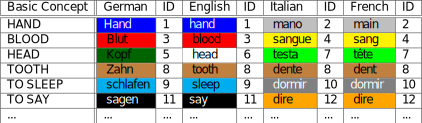
\includegraphics{img/cognates-1.svg}}

\subsection{\texorpdfstring{{Computergestützte
Rekonstruktion}}{Computergestützte Rekonstruktion}}

\subsubsection{\texorpdfstring{{Formate}}{Formate}}

\textbf{Distanzberechnung aus Swadeshlisten}

\href{img/distance-tree.png}{\includegraphics{img/distance-tree.png}}

\subsection{\texorpdfstring{{Computergestützte
Rekonstruktion}}{Computergestützte Rekonstruktion}}

\subsubsection{\texorpdfstring{{Formate}}{Formate}}

\textbf{Charaktermodellierung von Kognatensätzen}

\href{img/cognates-2.svg}{\includegraphics{img/cognates-2.svg}}

\subsection{\texorpdfstring{{Computergestützte
Rekonstruktion}}{Computergestützte Rekonstruktion}}

\subsubsection{\texorpdfstring{{Formate}}{Formate}}

\textbf{Charaktermodellierung von Kognatensätzen}

\href{img/character-tree.png}{\includegraphics{img/character-tree.png}}

\subsection{\texorpdfstring{{Computergestützte
Rekonstruktion}}{Computergestützte Rekonstruktion}}

\subsubsection{\texorpdfstring{{Formate}}{Formate}}

\textbf{Phylip-Format}

\begin{verbatim}
12
Germa 0.0 0.19 0.11 0.27 0.19 0.26 0.16 0.16 0.19 0.22 0.11 0.08
Engli 0.19 0.0 0.14 0.27 0.19 0.22 0.16 0.16 0.26 0.22 0.11 0.14
Dutch 0.11 0.14 0.0 0.29 0.21 0.27 0.14 0.18 0.24 0.24 0.13 0.09
Icela 0.27 0.27 0.29 0.0 0.08 0.21 0.14 0.11 0.27 0.08 0.22 0.22
Nynor 0.19 0.19 0.21 0.08 0.0 0.13 0.06 0.03 0.22 0.06 0.14 0.14
Riksm 0.26 0.22 0.27 0.21 0.13 0.0 0.13 0.09 0.29 0.16 0.21 0.21
Swedi 0.16 0.16 0.14 0.14 0.06 0.13 0.0 0.03 0.19 0.09 0.11 0.11
Danis 0.16 0.16 0.18 0.11 0.03 0.09 0.03 0.0 0.19 0.06 0.11 0.11
Gothi 0.19 0.26 0.24 0.27 0.22 0.29 0.19 0.19 0.0 0.22 0.18 0.18
OIcel 0.22 0.22 0.24 0.08 0.06 0.16 0.09 0.06 0.22 0.0 0.14 0.18
OEngl 0.11 0.11 0.13 0.22 0.14 0.21 0.11 0.11 0.18 0.14 0.0 0.06
OHGer 0.08 0.14 0.09 0.22 0.14 0.21 0.11 0.11 0.18 0.18 0.06 0.0
\end{verbatim}

\subsection{\texorpdfstring{{Computergestützte
Rekonstruktion}}{Computergestützte Rekonstruktion}}

\subsubsection{\texorpdfstring{{Formate}}{Formate}}

\textbf{Nexus-Format}

\begin{verbatim}
#nexus
BEGIN Taxa;
DIMENSIONS ntax=12;
TAXLABELS 'Germa' 'Engli' 'Dutch' 'Icela' 'Nynor' 'Riksm' 'Swedi' 'Danis'
'Gothi' 'OIcel' 'OEngl' 'OHGer';
END; [Taxa]
BEGIN Characters;
DIMENSIONS nchar=61;
FORMAT
datatype=STANDARD
missing=?
gap=-
symbols="01"
labels=left
transpose=no
interleave=no
;
MATRIX
'Germa' 0111111111111111111111111111111111111111100000000000000000000
'Engli' 0100011111111111111011111111010110111111111111000000000000000
'Dutch' 0101111111111111111111111111010111111111110010110000000000000
'Icela' 0100111110111111110111110111011110111111110001001111111100000
AH
'Nynor' 0100111110111111110111111111011110111111110001001110010000000
'Riksm' 0100010110111010111111011111011110111111110001001010010010000
'Swedi' 0100111110111111111111111111011110111111110001101010000000000
'Danis' 0100111110111111111111111111011110111111110001001010010000000
'Gothi' 0100111011111111111101110111011111111111100001001000000001111
'OIcel' 0100111110111111111111111111011110111111110001001111010101000
'OEngl' 0101111111111111111111111111011110111111110101000000000001000
'OHGer' 0101111111111111111111111111011111111111110100001000000000000
;
END;
\end{verbatim}

\subsection{\texorpdfstring{{Agenda 2015}}{Agenda 2015}}

\begin{itemize}
\itemsep1pt\parskip0pt\parsep0pt
\item
  {Phylogenetische Rekonstruktion}

  \begin{itemize}
  \itemsep1pt\parskip0pt\parsep0pt
  \item
    {Innere und äußere Sprachgeschichte}
  \item
    {Stammbäume und Wellen}
  \item
    {Darstellung und Analyse}
  \end{itemize}
\item
  {Lexikostatistik}

  \begin{itemize}
  \itemsep1pt\parskip0pt\parsep0pt
  \item
    {Hintergrund und Grundannahmen}
  \item
    {Praktische Umsetzung}
  \item
    {Kritik}
  \end{itemize}
\item
  {Computergestützte Rekonstruktion}

  \begin{itemize}
  \itemsep1pt\parskip0pt\parsep0pt
  \item
    {Komparanda}
  \item
    {Algorithmen}
  \item
    {Formate}
  \end{itemize}
\end{itemize}

\VERB|\NormalTok{>>> }\DecValTok{3} \NormalTok{- }\DecValTok{1}|

Ende der ersten Sitzung

\href{../slides.html}{ÜBERBLICK}

\hyperdef{}{changeme}{}{\href{../slides.html}{Nächste Sitzung}}

\hyperdef{}{changeve}{}{\href{../slides.html}{Vorherige Sitzung}}

Vorherige Sitzung

\section{Automatischer Sprachvergleich mit Python}
\hyperdef{}{tilda}{}

\subsection{Computergestützter Sprachvergleich mit Python und
JavaScript}

\begin{center}\rule{0.5\linewidth}{\linethickness}\end{center}

\subsubsection{Sitzung 2 (Tag 4)}

\begin{center}\rule{0.5\linewidth}{\linethickness}\end{center}

\paragraph{23.07.2015}

\begin{center}\rule{0.5\linewidth}{\linethickness}\end{center}

\subsubsection{\texorpdfstring{``Automatischer Sprachvergleich mit
Python''}{Automatischer Sprachvergleich mit Python}}

\subsection{\texorpdfstring{{Agenda 2015}}{Agenda 2015}}

\begin{itemize}
\itemsep1pt\parskip0pt\parsep0pt
\item
  {Automatischer Sprachvergleich}

  \begin{itemize}
  \itemsep1pt\parskip0pt\parsep0pt
  \item
    {Sequenzdistanzen}
  \item
    {Kognatenerkennung}
  \item
    {Phylogenetische Rekonstruktion}
  \end{itemize}
\item
  {Sprachvergleich mit LingPy}

  \begin{itemize}
  \itemsep1pt\parskip0pt\parsep0pt
  \item
    {Eingabeformate}
  \item
    {Analysen}
  \item
    {Ausgabeformate}
  \end{itemize}
\item
  {Workflows}

  \begin{itemize}
  \itemsep1pt\parskip0pt\parsep0pt
  \item
    {Allgemeines vorweg}
  \item
    {Kognatenerkennung mit LingPy}
  \item
    {Integration mit externen Tools}
  \end{itemize}
\end{itemize}

\subsection{\texorpdfstring{{Automatischer
Sprachvergleich}}{Automatischer Sprachvergleich}}

\subsubsection{\texorpdfstring{{Sequenzdistanzen}}{Sequenzdistanzen}}

\textbf{Von Alinierungen zu Distanzwerten}

Wenn man Sequenzen (Wörter im Falle der Linguistik) aliniert hat, dann
kann man auch ihre Distanz zueinander berechnen. Die ist implizit ja
bereits ein Teil der Berechnung der Alinierung, und sie kann
entsprechend auch einfach weiterverwendet werden, wobei man vorsichtig
sein sollte, was die Aussage einer solchen Distanz betrifft.

\subsection{\texorpdfstring{{Automatischer
Sprachvergleich}}{Automatischer Sprachvergleich}}

\subsubsection{\texorpdfstring{{Sequenzdistanzen}}{Sequenzdistanzen}}

\textbf{Die normalisierte Levenshtein-Distanz}

Eine der bekanntesten und am häufigsten verwendeten Distanzen zwischen
Strings ist die \emph{Levenshtein-Distanz}, die grundlegend die Anzahl
der \emph{Editier-Schritte} beschreibt, die notwendig sind, um eine
Sequenz in die andere zu überführen. Um eine bessere Vergleichbarkeit zu
gewährleisten, wird häufig neben der normalen
\emph{Levenshtein-Distanz}, die ein ganzzahliger Wert ist, auch die
``normalisierte Levenshtein-Distanz'' berechnet, bei der man die
``normale'' Distanz durch die Länge des größeren Strings teilt.

\subsection{\texorpdfstring{{Automatischer
Sprachvergleich}}{Automatischer Sprachvergleich}}

\subsubsection{\texorpdfstring{{Sequenzdistanzen}}{Sequenzdistanzen}}

\textbf{Die normalisierte Levenshtein-Distanz}

\begin{verbatim}
>>> from lingpy import *
>>> seqA = 'levensthein'
>>> seqB = 'levenschtein'
>>> d = edit_dist(seqA,seqB)
>>> d
1
>>> def norm_ed(a,b):
...     return edit_dist(a,b) / max(len(a), len(b))
...
>>> norm_ed(seqA, seqB)
0.08333333333333333
>>> edit_dist(seqA, seqB, normalized=True)
0.08333333333333333
\end{verbatim}

\subsection{\texorpdfstring{{Automatischer
Sprachvergleich}}{Automatischer Sprachvergleich}}

\subsubsection{\texorpdfstring{{Kognatenerkennung}}{Kognatenerkennung}}

\textbf{Automatisches Erkennen von kognaten Wörtern}

Kognaten sind, daran sei noch mal erinnert, Wörter, die auf einen
gemeinsamen Vorgänger zurückgehen (wie bspw. Deutsch \emph{Hand} und
English \emph{hand}). Automatisch können wir eine recht einfache
Heuristik entwickeln, um festzustellen, ob zwei Wörter kognat sind (was
nicht heißt, dass sie das auch wirklich sind!). Wir können einfach
sagen, dass, wenn immer zwei Wörter sich mehr ähneln als gewöhnlich, wir
annehmen, dass diese kognat sind. Die Ähnlichkeit können wir dabei
natürlich unterschiedlich definieren!

\subsection{\texorpdfstring{{Automatischer
Sprachvergleich}}{Automatischer Sprachvergleich}}

\subsubsection{\texorpdfstring{{Kognatenerkennung}}{Kognatenerkennung}}

\textbf{Die Lautklassenheuristik}

Eine erste einfache Heuristik besagt, dass zwei Wörter immer dann als
kognat klassifiziert werden, wenn sie in den ersten beiden Lautklassen,
die Konsonanten sind, übereinstimmen
(\href{http://bibliography.lingpy.org?key=Turchin2010}{Turchin et al.
2010}).

\begin{verbatim}
>>> seqA = sampa2uni('Tri')
>>> seqB = sampa2uni('drai')
>>> seqA, seqB 
('θri', 'drai')
>>> clsA = tokens2class(ipa2tokens(seqA), 'dolgo')
>>> clsB = tokens2class(ipa2tokens(seqB), 'dolgo')
>>> clsA = ''.join(clsA).replace('V','')
>>> clsB = ''.join(clsB).replace('V','')
>>> clsA[:2] == clsB[:2]
True
>>> clsA, clsB
('TR', 'TR')
>>> turchin(seqA, seqB)
0
>>> turchin(seqA, 'test')
1
\end{verbatim}

\subsection{\texorpdfstring{{Automatischer
Sprachvergleich}}{Automatischer Sprachvergleich}}

\subsubsection{\texorpdfstring{{Kognatenerkennung}}{Kognatenerkennung}}

\textbf{Schwellenwerte}

Anstelle des Kriteriums von
\href{http://bibliography.lingpy.org?key=Turchin2010}{Turchin et al.
(2010)} könnenwir natürlich auch andere Verfahren verwenden. Zum
Beispiel können wir sagen, dass ab einem bestimmten Schwellenwert der
normalisierten Levenshtein-Distanz zwei Wörter nicht mehr kognat sind:

\begin{verbatim}
>>> def cognate(seqA, seqB, threshold=0.4):
...     if edit_dist(seqA, seqB, normalized=True) > threshold:
...         return 1
...     return 0
... 
>>> seqA = sampa2uni('t_hOxt@r')
>>> seqB = 
KeyboardInterrupt
>>> seqA = sampa2uni('t_hOxt_h@r')
>>> seqB = sampa2uni('dO:t_h@r')
>>> cognate(seqA, seqB)
\end{verbatim}

\subsection{\texorpdfstring{{Automatischer
Sprachvergleich}}{Automatischer Sprachvergleich}}

\subsubsection{\texorpdfstring{{Phylogenetische
Rekonstruktion}}{Phylogenetische Rekonstruktion}}

\textbf{Von Distanzen zu Bäumen}

Wenn wir ermittelt haben, welche Wörter in welchen Sprachen miteinander
kognat sind, können wir Distanzen zwischen ganzen Sprachen berechnen.
Dazu zählen wir einfach alle kognaten Wörter in unserem Sample und
teilen dann die Anzahl der kognaten Wörter durch die Gesamt-Anzahl der
Wörter und ziehen diesen Wert von 1 ab (ansonsten hätten wir eine
Ähnlichkeit und keine Distanzen).

\subsection{\texorpdfstring{{Automatischer
Sprachvergleich}}{Automatischer Sprachvergleich}}

\subsubsection{\texorpdfstring{{Phylogenetische
Rekonstruktion}}{Phylogenetische Rekonstruktion}}

\textbf{Kleines Beispiel zur Distanzberechnung}

\begin{verbatim}
from lingpy import *
# die daten
data = dict(
    german = ['hant', 'fuːs', 'kɔp͡f'],
    english = ['hænd', 'fʊt', 'hɛd'],
    dutch = ['hant', 'vut', 'kɔp']
    )
# die sprachen
taxa = ['german', 'english', 'dutch']
# die distanzmatrix
matrix = [[0 for i in range(3)] for j in range(3)]
for i,k in enumerate(taxa):
    for j,l in enumerate(taxa):
        # wir müssen nur ein mal pro sprachpaar vergleichen
        if i < j:
            score = 0
            for seqA, seqB in zip(data[k], data[l]):
                score += edit_dist(seqA, seqB, normalized=True)
            score = score / 3
            matrix[i][j] = score
            matrix[j][i] = score
# der baum
tree = upgma(matrix, taxa)
# ascii-art mit Hilfe von LingPy
print(Tree(tree).asciiArt())
\end{verbatim}

\subsection{\texorpdfstring{{Automatischer
Sprachvergleich}}{Automatischer Sprachvergleich}}

\subsubsection{\texorpdfstring{{Phylogenetische
Rekonstruktion}}{Phylogenetische Rekonstruktion}}

\textbf{Kleines Beispiel zur Distanzberechnung}

\begin{verbatim}
$ python distances.py
          /-english
-root----|
         |          /-german
          \edge.0--|
                    \-dutch
\end{verbatim}

\subsection{\texorpdfstring{{Agenda 2015}}{Agenda 2015}}

\begin{itemize}
\itemsep1pt\parskip0pt\parsep0pt
\item
  {Automatischer Sprachvergleich}

  \begin{itemize}
  \itemsep1pt\parskip0pt\parsep0pt
  \item
    {Sequenzdistanzen}
  \item
    {Kognatenerkennung}
  \item
    {Phylogenetische Rekonstruktion}
  \end{itemize}
\item
  {Sprachvergleich mit LingPy}

  \begin{itemize}
  \itemsep1pt\parskip0pt\parsep0pt
  \item
    {Eingabeformate}
  \item
    {Analysen}
  \item
    {Ausgabeformate}
  \end{itemize}
\item
  {Workflows}

  \begin{itemize}
  \itemsep1pt\parskip0pt\parsep0pt
  \item
    {Allgemeines vorweg}
  \item
    {Kognatenerkennung mit LingPy}
  \item
    {Integration mit externen Tools}
  \end{itemize}
\end{itemize}

\subsection{\texorpdfstring{{Sprachvergleich mit
LingPy}}{Sprachvergleich mit LingPy}}

\subsubsection{\texorpdfstring{{Eingabeformate}}{Eingabeformate}}

\textbf{Basisformat für Wortlisten}

\begin{verbatim}
ID   CONCEPT     COUNTERPART   IPA         DOCULECT     COGID
1    hand        Hand          hant        German       1
2    hand        hand          hænd        English      1
3    hand        рука          ruka        Russian      2
4    hand        рука          ruka        Ukrainian    2
5    leg         Bein          bain        German       3
6    leg         leg           lɛg         English      4
7    leg         нога          noga        Russian      5
8    leg         нога          noha        Ukrainian    5
9    Woldemort   Waldemar      valdemar    German       6
10   Woldemort   Woldemort     wɔldemɔrt   English      6
11   Woldemort   Владимир      vladimir    Russian      6
12   Woldemort   Володимир     volodimir   Ukrainian    6
13    Harry       Harald        haralt      German       7
14   Harry       Harry         hæri        English      7
15   Harry       Гарри         gari        Russian      7
16   Harry       Гаррi         hari        Ukrainian    7
\end{verbatim}

\subsection{\texorpdfstring{{Sprachvergleich mit
LingPy}}{Sprachvergleich mit LingPy}}

\subsubsection{\texorpdfstring{{Eingabeformate}}{Eingabeformate}}

\textbf{Key-Value-Erweiterung des Basisformats}

\begin{verbatim}
#
ID   CONCEPT     COUNTERPART   IPA         DOCULECT     COGID    ALIGNMENT
1    hand        Hand          hant        German       1        
2    hand        hand          hænd        English      1        
3    hand        рука          ruka        Russian      2        
...  ...         ...           ...         ...          ...      ...
\end{verbatim}

\subsection{\texorpdfstring{{Sprachvergleich mit
LingPy}}{Sprachvergleich mit LingPy}}

\subsubsection{\texorpdfstring{{Eingabeformate}}{Eingabeformate}}

\textbf{Darstellung von Alinierungen}

\begin{verbatim}
#
ID   CONCEPT     COUNTERPART   IPA         DOCULECT     COGID   ALIGNMENT  
...  ...         ...           ...         ...          ...     ...  
9    Woldemort   Waldemar      valdemar    German       6       v a l - d e m a r -
10   Woldemort   Woldemort     wɔldemɔrt   English      6       w ɔ l - d e m ɔ r t 
11   Woldemort   Владимир      vladimir    Russian      6       v - l a d i m i r -
12   Woldemort   Володимир     volodimir   Ukrainian    6       v o l o d i m i r -
...  ...         ...           ...         ...          ...     ...  
\end{verbatim}

\subsection{\texorpdfstring{{Sprachvergleich mit
LingPy}}{Sprachvergleich mit LingPy}}

\subsubsection{\texorpdfstring{{Analysen}}{Analysen}}

\textbf{Kognatenerkennung mit LexStat}

Kognatenerkennung in LingPy lässt sich mit Hilfe des
\href{http://lingpy.org/reference/lingpy.compare.html\#module-lingpy.compare.lexstat}{LexStat-Moduls}
durchführen. Basierend auf einer Datei, die das oben beschriebene
Eingabeformat aufweist und zwingend die Spalten ``CONCEPT'', ``IPA'',
und ``DOCULECT'' enthalten muss, kann man mit Hilfe des LexStat-Moduls
Kognaten auf verschiedene Art und Weise berechnen, diese Werte dann in
Distanzen umwandeln, und aus den Distanzen auch direkt einen Baum
berechnen.

\subsection{\texorpdfstring{{Sprachvergleich mit
LingPy}}{Sprachvergleich mit LingPy}}

\subsubsection{\texorpdfstring{{Analysen}}{Analysen}}

\textbf{Beispiel zur Kognatenerkennung mit LexStat}

\begin{verbatim}
>>> from lingpy import *
>>> lex = LexStat('data/harry.tsv')
>>> lex.cluster(method='turchin')
>>> lex.cluster(method='turchin')
|++++++++++++++++++++++++++++++++++++++++++++++++++++++++++++++++++++++++++++++++++++++++++++++++++++|
>>> lex.calculate(tree, ref="turchinid")
>>> print(lex.tree.asciiArt())
                    /-English
          /edge.0--|
         |          \-German
-root----|
         |          /-Russian
          \edge.1--|
                    \-Ukrainian
\end{verbatim}

\subsection{\texorpdfstring{{Sprachvergleich mit
LingPy}}{Sprachvergleich mit LingPy}}

\subsubsection{\texorpdfstring{{Analysen}}{Analysen}}

\textbf{Alinierung von Kognatensets}

Es ist sinnvoll, die automatisch ermittelten Kognaten auch zu alinieren,
da man sich so am besten vergewsissern kann, dass man auch keine
falschen Kognaten ermittelt oder richtige Kognaten übersehen hat.
Hierfür bietet sich das
\href{http://lingpy.org/reference/lingpy.align.html\#module-lingpy.align.sca}{SCA-Modul}
von LingPy an, welches als Eingabe eine Wortliste nimmt und neben den
für LexStat geforderten Spalten ``DOCULECT'', ``CONCEPT'' und ``IPA''
eine weitere Spalte erfordert, die dem Programm mitteilt, wo die
Kognaten-Identifikationsnummern sind. Normalerweise werden diese Spalten
in LingPy nach der Methode beziffert, die ihnen zugrunde liegt
(``turchin'' == ``turchinid'', ``sca'' == ``scaid'', etc.), wobei der
Name ``cogid'' gewöhnlich für eine von Experten ermittelte
Kognatenzuweisung reserviert wird.

\subsection{\texorpdfstring{{Sprachvergleich mit
LingPy}}{Sprachvergleich mit LingPy}}

\subsubsection{\texorpdfstring{{Analysen}}{Analysen}}

\textbf{Beispiel für die Alinierung von Kognatensets}

\begin{verbatim}
>>> from lingpy import *
>>> alm = Alignments('data/harry.tsv', ref="cogid")
>>> alm.align()
|--------------------------- ALIGNMENTS --------------------------------|
>>> alm.output('html', filename='data/harry')
\end{verbatim}

\subsection{\texorpdfstring{{Sprachvergleich mit
LingPy}}{Sprachvergleich mit LingPy}}

\subsubsection{\texorpdfstring{{Analysen}}{Analysen}}

\textbf{Ausgabe der Daten in HTML-Format}

\subsection{\texorpdfstring{{Sprachvergleich mit
LingPy}}{Sprachvergleich mit LingPy}}

\subsubsection{\texorpdfstring{{Ausgabeformate}}{Ausgabeformate}}

\textbf{Grundlegendes zu Ausgabeformaten in LingPy}

Daten in LingPy können in verschiedenste Formate exportiert werden.
Grundlegend unterscheiden können wir dabei zwei Formattypen:

\begin{itemize}
\itemsep1pt\parskip0pt\parsep0pt
\item
  Endformate, die entweder für Publikationen oder zur manuellen
  Untersuchung von Ergebnissen verwendet werden können (Plots,
  Grafiken), und
\item
  Übergangsformate, die zur Weiterverwendung in alternativen
  Softwarepackungen verwendet werden können.
\end{itemize}

\subsection{\texorpdfstring{{Sprachvergleich mit
LingPy}}{Sprachvergleich mit LingPy}}

\subsubsection{\texorpdfstring{{Ausgabeformate}}{Ausgabeformate}}

\textbf{Spezifizieren von Ausgabeformaten in LingPy}

\begin{verbatim}
# grundlegenes Format des Kommandos
wordlist.output(DTYPE, filename=NAME)
# Beispiele
## Exportiere nach Phylip (Distanzformat)
wordlist.output('dst', filename="harry")
## Exportiere nach Nexus (Charakterformat)
wordlist.output('paps.nex', filename="harry")
## Exportiere nach HTML (individuelles LingPy-Format)
wordlist.output('html', filename="harry")
## Exportiere den Baum in Newick-Format
wordlist.output('nwk', filename="harry")
## Exportiere zum LingPy-Wordlist-Format
wordlist.output('tsv', filename='harry')
\end{verbatim}

\subsection{\texorpdfstring{{Sprachvergleich mit
LingPy}}{Sprachvergleich mit LingPy}}

\subsubsection{\texorpdfstring{{Ausgabeformate}}{Ausgabeformate}}

\textbf{Beispiele für die Ausgabeformate}

Newick-Format:

\begin{verbatim}
(((English,German),Russian),Ukrainian);
\end{verbatim}

Phylip-Format:

\begin{verbatim}
 4
English    0.00 0.25 0.50 0.50
German     0.25 0.00 0.50 0.50
Russian    0.50 0.50 0.00 0.00
Ukrainian  0.50 0.50 0.00 0.00
\end{verbatim}

\subsection{\texorpdfstring{{Sprachvergleich mit
LingPy}}{Sprachvergleich mit LingPy}}

\subsubsection{\texorpdfstring{{Ausgabeformate}}{Ausgabeformate}}

\textbf{Beispiele für die Ausgabeformate}

Nexus-Format:

\begin{verbatim}
#NEXUS
BEGIN DATA;
DIMENSIONS ntax=4 NCHAR=7;
FORMAT DATATYPE=STANDARD GAP=- MISSING=0 interleave=yes;
MATRIX
English   1001011
German    1010011
Russian   0100111
Ukrainian 0100111
;
END;
\end{verbatim}

\subsection{\texorpdfstring{{Agenda 2015}}{Agenda 2015}}

\begin{itemize}
\itemsep1pt\parskip0pt\parsep0pt
\item
  {Automatischer Sprachvergleich}

  \begin{itemize}
  \itemsep1pt\parskip0pt\parsep0pt
  \item
    {Sequenzdistanzen}
  \item
    {Kognatenerkennung}
  \item
    {Phylogenetische Rekonstruktion}
  \end{itemize}
\item
  {Sprachvergleich mit LingPy}

  \begin{itemize}
  \itemsep1pt\parskip0pt\parsep0pt
  \item
    {Eingabeformate}
  \item
    {Analysen}
  \item
    {Ausgabeformate}
  \end{itemize}
\item
  {Workflows}

  \begin{itemize}
  \itemsep1pt\parskip0pt\parsep0pt
  \item
    {Allgemeines vorweg}
  \item
    {Kognatenerkennung mit LingPy}
  \item
    {Integration mit externen Tools}
  \end{itemize}
\end{itemize}

\subsection{\texorpdfstring{{Workflows}}{Workflows}}

\subsubsection{\texorpdfstring{{Allgemeines
vorweg}}{Allgemeines vorweg}}

\textbf{Workflows in LingPy}

Mit Hilfe der Funktionen, die LingPy bietet, lassens ich komplette
Workflows zum automatisierten Vergleich von Sprachen entwickeln. Das ist
nicht immer einfach, da nur ein Bruchteil der Möglichkeiten von LingPy
auch ordentlich dokumentiert ist. Wir wollen aber trotzdem versuchen,
ein allgemeines Template zu erstellen, so dass es möglich ist, dieses an
individuelle Daten anzupassen und weiterzuverwenden.

\subsection{\texorpdfstring{{Workflows}}{Workflows}}

\subsubsection{\texorpdfstring{{Allgemeines
vorweg}}{Allgemeines vorweg}}

\textbf{Workflows zum Sprachvergleich}

\begin{longtable}[c]{@{}ll@{}}
\toprule
\href{img/workflow_basic.svg}{\includegraphics{img/workflow_basic.svg}}
& Dieser Workflow kann als allgemeines Konstrukt der von rohen Daten bis
hin zu Rekonstruktionen führt, angesehen werden. Nicht alle Schritte
können derzeit schon automatisch ausgeführt werden. Wir beschränken uns
daher auf die Schritte, die von den Wortlist-Daten hin zu den
Alinierungen führen.\tabularnewline
\bottomrule
\end{longtable}

\subsection{\texorpdfstring{{Workflows}}{Workflows}}

\subsubsection{\texorpdfstring{{Kognatenerkennung mit
LingPy}}{Kognatenerkennung mit LingPy}}

\textbf{Daten}

Wir nehmen einen Datensatz zu den chinesischen Dialekten, der als
TSV-Datei im LingPy Format vorliegt (File
"\href{https://github.com/LinguList/pyjs-seminar/blob/master/website/code/data/chinese.tsv}{chinese.tsv}").

Die Datei enthält neben den tabularen Daten auch eine JSON-Spezifikation
(eine Formaterweiterung in LingPy, die es erlaubt, JSON-Daten mit
einzubinden. Wir ignorieren diese Daten jedoch in diesem Zusammenhang.

\subsection{\texorpdfstring{{Workflows}}{Workflows}}

\subsubsection{\texorpdfstring{{Kognatenerkennung mit
LingPy}}{Kognatenerkennung mit LingPy}}

\textbf{Der Workflow}

Der Workflow gliedert sich in drei Schritte:

\begin{itemize}
\itemsep1pt\parskip0pt\parsep0pt
\item
  Kognatenberechnung:

  \begin{itemize}
  \itemsep1pt\parskip0pt\parsep0pt
  \item
    Einlesen der Datei in LingPy (LexStat Modul)
  \item
    Berechnen von Kognatensets mit Hilfe von LexStat
  \item
    Auslesen der Datei mit den neu berechneten Daten in TSV-Format
  \end{itemize}
\item
  Berechnen und Plotten eines phylogenetischen Baums
\item
  Berechnung der Alinierungen

  \begin{itemize}
  \itemsep1pt\parskip0pt\parsep0pt
  \item
    Einlesen der Datei in LingPy (Alignments Modul)
  \item
    Berechnen der Alinierungen mit Hilfe von Alignments
  \item
    Auslesen der Datei in HTML-Format
  \end{itemize}
\end{itemize}

\subsection{\texorpdfstring{{Workflows}}{Workflows}}

\subsubsection{\texorpdfstring{{Kognatenerkennung mit
LingPy}}{Kognatenerkennung mit LingPy}}

\textbf{Der Code}

\begin{verbatim}
from lingpy import *
# Schritt 1
## 1.1 Einlesen der Daten
lex = LexStat('data/chinese.tsv')
## 1.2 Kognatenerkennung
lex.cluster(method='sca', threshold=0.4)
## 1.3 Auslesen der Daten
lex.output('tsv', filename='data/chinese_lexstat', ignore='all')
# Schritt 2
## 1.1 Berechnen des Baums
lex.calculate('tree', ref="scaid") # scaid sind die automatischen kognaten
## 1.2 Plotten des Baums
from lingpy.convert.plot import plot_tree
plot_tree(lex.tree, degree=160, filename="data/chinese_tree", fileformat="svg")
## 1.3 Schreiben der Distanz-Daten
lex.output('dst', filename="data/chinese_distances")
# Schritt 3
## 1.1 Einlesen der Daten
alm = Alignments('data/chinese_lexstat.tsv', ref="scaid")
## 1.2 Alinierung
alm.align()
## 1.3 Auslesen der Daten in HTML
alm.output('html', filename='data/chinese_alignments')
\end{verbatim}

\subsection{\texorpdfstring{{Workflows}}{Workflows}}

\subsubsection{\texorpdfstring{{Kognatenerkennung mit
LingPy}}{Kognatenerkennung mit LingPy}}

\textbf{Die Ergebnisse: Der Baum}

\href{../code/data/chinese_tree.svg}{\includegraphics{../code/data/chinese_tree.svg}}

\subsection{\texorpdfstring{{Workflows}}{Workflows}}

\subsubsection{\texorpdfstring{{Kognatenerkennung mit
LingPy}}{Kognatenerkennung mit LingPy}}

\textbf{Die Ergebnisse: Die Alinierungen}

\subsection{\texorpdfstring{{Workflows}}{Workflows}}

\subsubsection{\texorpdfstring{{Integration mit externen
Tools}}{Integration mit externen Tools}}

\textbf{Einlesen der Daten in Splitstree}

Mit \href{http://splitstree.org}{SplitsTree} können wir Netzwerke aus
Distanzmatrizzen berechnen. Da wir die Distanzmatrix ja bereits
exportiert haben, genügt es, wenn SplitStree erfolgreich installiert
wurde, diese entweder direkt als Textdatei einzulesen, oder den Inhalt
der Datei
\href{ttps://github.com/LinguList/pyjs-seminar/blob/master/website/code/data/chinese_distances.dst}{chinese\_distances.dst}
zu kopieren und in den Editor von SplitsTree zu pasten.

\subsection{\texorpdfstring{{Workflows}}{Workflows}}

\subsubsection{\texorpdfstring{{Integration mit externen
Tools}}{Integration mit externen Tools}}

\textbf{Das Neighbor-Net der chinesischen Daten}

\href{../code/data/chinese_network.svg}{\includegraphics{../code/data/chinese_network.svg}}

\subsection{\texorpdfstring{{Agenda 2015}}{Agenda 2015}}

\begin{itemize}
\itemsep1pt\parskip0pt\parsep0pt
\item
  {Automatischer Sprachvergleich}

  \begin{itemize}
  \itemsep1pt\parskip0pt\parsep0pt
  \item
    {Sequenzdistanzen}
  \item
    {Kognatenerkennung}
  \item
    {Phylogenetische Rekonstruktion}
  \end{itemize}
\item
  {Sprachvergleich mit LingPy}

  \begin{itemize}
  \itemsep1pt\parskip0pt\parsep0pt
  \item
    {Eingabeformate}
  \item
    {Analysen}
  \item
    {Ausgabeformate}
  \end{itemize}
\item
  {Workflows}

  \begin{itemize}
  \itemsep1pt\parskip0pt\parsep0pt
  \item
    {Allgemeines vorweg}
  \item
    {Kognatenerkennung mit LingPy}
  \item
    {Integration mit externen Tools}
  \end{itemize}
\end{itemize}

\VERB|\NormalTok{>>> }\DecValTok{3} \NormalTok{- }\DecValTok{2}|

Ende der zweiten Sitzung

\href{../slides.html}{ÜBERBLICK}

\hyperdef{}{changeme}{}{\href{../slides.html}{Nächste Sitzung}}

\hyperdef{}{changeve}{}{\href{../slides.html}{Vorherige Sitzung}}

Vorherige Sitzung

\section{Geoplots mit JavaScript und D3}
\hyperdef{}{tilda}{}

\subsection{Computergestützter Sprachvergleich mit Python und
JavaScript}

\begin{center}\rule{0.5\linewidth}{\linethickness}\end{center}

\subsubsection{Sitzung 3 (Tag 4)}

\begin{center}\rule{0.5\linewidth}{\linethickness}\end{center}

\paragraph{23.07.2015}

\begin{center}\rule{0.5\linewidth}{\linethickness}\end{center}

\subsubsection{\texorpdfstring{``Geoplots mit JavaScript und
D3''}{Geoplots mit JavaScript und D3}}

\subsection{\texorpdfstring{{Agenda 2015}}{Agenda 2015}}

\begin{itemize}
\itemsep1pt\parskip0pt\parsep0pt
\item
  {Darstellung geographischer Daten}

  \begin{itemize}
  \itemsep1pt\parskip0pt\parsep0pt
  \item
    {GeoJson und TopoJson}
  \item
    {D3}
  \end{itemize}
\item
  {Eine Beispielapplikation}

  \begin{itemize}
  \itemsep1pt\parskip0pt\parsep0pt
  \item
    {Idee}
  \item
    {Vorbereitung}
  \item
    {Applikation}
  \end{itemize}
\end{itemize}

\subsection{\texorpdfstring{{Darstellung geographischer
Daten}}{Darstellung geographischer Daten}}

\subsubsection{\texorpdfstring{{GeoJson und
TopoJson}}{GeoJson und TopoJson}}

\textbf{Grundlegendes}

\href{http://geojson.org}{GeoJson} und
\href{https://github.com/mbostock/topojson}{TopoJson} sind Formate zur
einfachen Beschreibung geographischer Daten. Sie bauen beide auf dem
JSON-Format auf, welches wir im Laufe des Woche ja schon zuweilen
verwendet haben. Beide Formate stellen eine ideale Grundlage für
geographische Darstellungen mit JavaScript dar und sind auch ineinander
überführbar. Wir werden TopoJson für unser Beispiel verwenden.

\subsection{\texorpdfstring{{Darstellung geographischer
Daten}}{Darstellung geographischer Daten}}

\subsubsection{\texorpdfstring{{GeoJson und
TopoJson}}{GeoJson und TopoJson}}

\textbf{GitHub-Integration}

\begin{itemize}
\item
  Das tolle an Geo- und TopoJson ist, dass die Formate direkt in GitHub
  als Karten dargestellt werden.
\item
  Wenn wir uns Beispielsweise die Datei
  \href{https://github.com/LinguList/pyjs-seminar/blob/master/website/demos/china/maps/zh-mainland-provinces.topo.json}{zh-mainland-provinces-topo.json}
  direkt auf GitHub anschauen, dann sehen wir direkt eine Karte, und
  auch, was auf der Karte zu sehen ist!
\end{itemize}

\subsection{\texorpdfstring{{Darstellung geographischer
Daten}}{Darstellung geographischer Daten}}

\subsubsection{\texorpdfstring{{GeoJson und
TopoJson}}{GeoJson und TopoJson}}

\textbf{Getting Started}

Grundlegendes zu den Formaten, aber auch zum Gestalten einer Karte kann
man im Internet in vielen Beispielen finden. Ich selbst habe meine
ersten Erkenntnisse über D3 und die Verwendung von geographischen Daten
in JS durch das Beispiel \href{http://bost.ocks.org/mike/map/}{Let's
Make a Map} von Mike Bostock gesammelt.

Dort beschreibt Bostock auch, wo man gute geographischen Daten finden
kann. Diese liegen meist in Form von ``shapefiles'' vor, die nicht in JS
verwendet werden können. Aber es gibt mit
\href{http://mapshaper.org/}{mapshaper} ein sehr gutes Tool, um die
Daten direkt in die JSON-Formate umzuwandeln.

\subsection{\texorpdfstring{{Darstellung geographischer
Daten}}{Darstellung geographischer Daten}}

\subsubsection{\texorpdfstring{{D3}}{D3}}

\href{http://d3js.org}{D3} ist eine wunderbare Bibliothek, um Daten zu
Visualisieren und interaktive Applikationen zu schreiben. Leider ist sie
auch sehr kompliziert und für Anfänger nur schwer zugänglich, da sich
hinter dem Kode viele sehr sinnvolle aber auch eigenwillige Konzepte
verbergen.

Wir haben in diesem Seminar leider keine Zeit, voll auf D3 und die
Möglichkeiten einzugehen. Wir werden uns daher auf ein Beispiel
beschränken, in dem es weniger um den Kode als um die Idee der
Visualisierung geht.

Denjenigen, die mehr über D3 erfahren möchte, empfehle ich, mit der
\href{http://d3js.org}{offiziellen Homepage} anzufangen, und sich dann
langsam ``hochzuarbeiten''.

\subsection{\texorpdfstring{{Agenda 2015}}{Agenda 2015}}

\begin{itemize}
\itemsep1pt\parskip0pt\parsep0pt
\item
  {Darstellung geographischer Daten}

  \begin{itemize}
  \itemsep1pt\parskip0pt\parsep0pt
  \item
    {GeoJson und TopoJson}
  \item
    {D3}
  \end{itemize}
\item
  {Eine Beispielapplikation}

  \begin{itemize}
  \itemsep1pt\parskip0pt\parsep0pt
  \item
    {Idee}
  \item
    {Vorbereitung}
  \item
    {Applikation}
  \end{itemize}
\end{itemize}

\subsection{\texorpdfstring{{Eine
Beispielapplikation}}{Eine Beispielapplikation}}

\subsubsection{\texorpdfstring{{Idee}}{Idee}}

\textbf{Die Daten}

Wir haben uns schon mit der Kollektion chinesischer Daten befasst und
sie sogar bereits mit Hilfe von LingPy aliniert. Nun wollen wir einen
Schritt weiter gehen, und die Diversität der Sprachen nicht nur über die
einzelnen Alinierungen, sondern auch im Raum darzustellen.

\subsection{\texorpdfstring{{Eine
Beispielapplikation}}{Eine Beispielapplikation}}

\subsubsection{\texorpdfstring{{Idee}}{Idee}}

\textbf{Die Idee}

Die Idee ist einfach: Wir plotten alle Dialektpunkte auf eine Karte, und
erlauben dann den Benutzern, Konzeptweise Daten aufzurufen und bei Klick
auf einen Dialektpunkt sowohl die Verteilung des Kognatensets als auch
die Wörter in alinierter Form zu betrachten.

\subsection{\texorpdfstring{{Eine
Beispielapplikation}}{Eine Beispielapplikation}}

\subsubsection{\texorpdfstring{{Idee}}{Idee}}

\textbf{Die Tools}

\begin{itemize}
\itemsep1pt\parskip0pt\parsep0pt
\item
  Python: zur Alinierung der Daten und zur Aufbereitung der Daten in
  JavaScript-kompatible Formate (JSON, JS Objekte).
\item
  JavaScript: zum Plotten der Daten mit Hilfe von D3.
\end{itemize}

\subsection{\texorpdfstring{{Eine
Beispielapplikation}}{Eine Beispielapplikation}}

\subsubsection{\texorpdfstring{{Vorbereitung}}{Vorbereitung}}

\textbf{Programmarbeit}

\begin{itemize}
\itemsep1pt\parskip0pt\parsep0pt
\item
  Erstellen der Daten und Überführung in LingPy-Wortlisten-Format
\item
  Durchführung der Alinierungsanalyse mit Hilfe von LingPy
\item
  Exportieren der Daten in JS-Formate (hauptsächlich JS-Objects, die ja
  wie ein Hash verwendet werden können und identisch mit JSON-Objekten
  sind).
\end{itemize}

\subsection{\texorpdfstring{{Eine
Beispielapplikation}}{Eine Beispielapplikation}}

\subsubsection{\texorpdfstring{{Vorbereitung}}{Vorbereitung}}

\textbf{Hintergrundarbeit}

\begin{itemize}
\itemsep1pt\parskip0pt\parsep0pt
\item
  Geographische Files konnten übernommen werden aus einem
  \href{https://github.com/clemsos/d3-china-map}{GitHub-Repository}.
\item
  Der Kode musste nur geringfügig angepasst werden, und die
  Dialektpunkte ergänzt werden.
\end{itemize}

\subsection{\texorpdfstring{{Eine
Beispielapplikation}}{Eine Beispielapplikation}}

\subsubsection{\texorpdfstring{{Vorbereitung}}{Vorbereitung}}

\textbf{Planung der Applikation}

\begin{itemize}
\itemsep1pt\parskip0pt\parsep0pt
\item
  Grundlegende Idee: Teile die Applikation in zwei Teile, einen mit der
  Karte, einen mit den Alinierungen
\item
  Zur Darstellung der Alinierungen liegt bereits eine
  \href{http://github.com/dighl/prison}{JS-Bibliothek} vor, die es
  ermöglicht, Wörter, die segmentiert vorliegen, koloriert darzustellen.
\item
  Erweiterte Ideen wurden in einem nicht ratsamen
  ``trial-and-error-Vefahren'' entwickelt (planen ist immer besser als
  ausprobieren, aber man plant dann am Ende doch immer viel zu
  wenig\ldots{}).
\end{itemize}

\subsection{\texorpdfstring{{Eine
Beispielapplikation}}{Eine Beispielapplikation}}

\subsubsection{\texorpdfstring{{Applikation}}{Applikation}}

\subsection{\texorpdfstring{{Agenda 2015}}{Agenda 2015}}

\begin{itemize}
\itemsep1pt\parskip0pt\parsep0pt
\item
  {Darstellung geographischer Daten}

  \begin{itemize}
  \itemsep1pt\parskip0pt\parsep0pt
  \item
    {GeoJson und TopoJson}
  \item
    {D3}
  \end{itemize}
\item
  {Eine Beispielapplikation}

  \begin{itemize}
  \itemsep1pt\parskip0pt\parsep0pt
  \item
    {Idee}
  \item
    {Vorbereitung}
  \item
    {Applikation}
  \end{itemize}
\end{itemize}

\VERB|\NormalTok{>>> }\DecValTok{3} \NormalTok{- }\DecValTok{3}|

Ende des Blockseminars

\href{../slides.html}{ÜBERBLICK}

\hyperdef{}{changeme}{}{\href{../slides.html}{Nächste Sitzung}}

\hyperdef{}{changeve}{}{\href{../slides.html}{Vorherige Sitzung}}

Vorherige Sitzung


\end{document}

